% #####################################################
% #####################################################
% #####################################################
\setchapterimage[3cm]{figures/chap3/chapter_head_LHRF} % Optionally specify theheight
\setchapterpreamble[u]{\margintoc}
\chapter[High Power RF Devices for the Lower Hybrid Range of Frequency]{High Power RF Devices for the LHRF}\label{eq:LHRF_work}

\setlength{\epigraphwidth}{.7\textwidth}
\epigraph{Les sciences ne sont pas comme Minerve, qui sortit tout armée du cerveau de Jupiter ; elles sont filles du temps, et se forment insensiblement, d’abord par la collection des méthodes indiquées par l’expérience, et plus tard par la découverte des principes qui se déduisent de la combinaison de ces méthodes. }{Brillat-Savarin, Physiologie du goût.}


This chapter reviews the work done by the author on high power RF devices at CEA/IRFM for the Lower Hybrid Range of frequencies. After a general introduction on LHRF systems in Section~\ref{sec:LHCD_antennas_general}, the Section~\ref{eq:LHRF_work} review the ITER LHCD antenna (Section~\ref{sec:ITER_LHCD_antenna}). Because it is needed to bring the RF power up to the antenna, high power transmission line elements are also necessary. Work performed on the design and tests of few kinds of high power devices such as a mode converter, vacuum windows are detailed in Chapter. 


% #####################################################
% #####################################################
% #####################################################
\section[Generalities]{Generalities on LHCD Antennas}\label{sec:LHCD_antennas_general}
\marginnote{Part of this section are taken from \citeauthyear{hillairet2012-1} and \citeauthyear{hillairet2020-1}.}

% #####################################################
% #####################################################
\subsection{“Grill” Antennas}
%\todo{fast wave coupling : electric field in the waveguide need to be directed polodally. But N//>1 so dielectric filled waveguide, problem.}
As the plasma cross-section dimensions of toroidal devices became sufficiently large to accommodate the free space wavelength at the lower hybrid frequencies, it becomes possible to couple the RF power directly by open-ended waveguides inserted in the vacuum vessel wall, thus avoiding coils or antennas within the vacuum chamber (Figure~\ref{fig:compassgrillout}).

\begin{marginfigure}
	\centering
	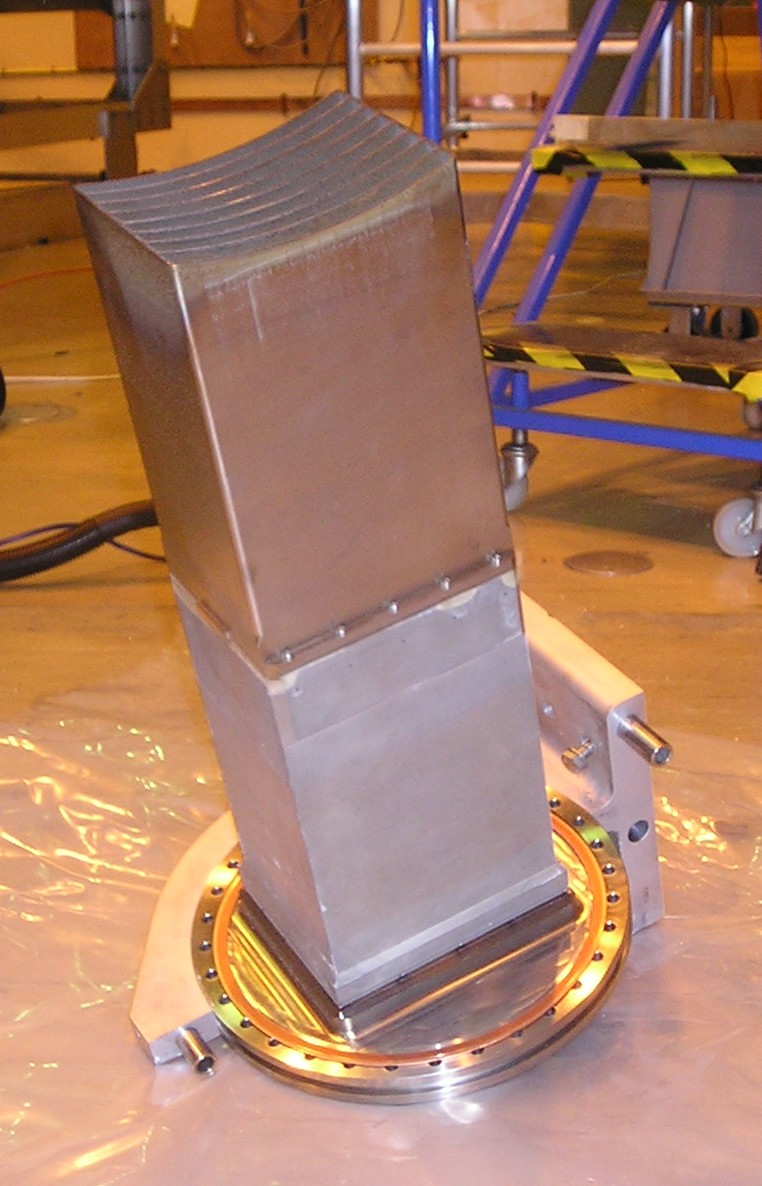
\includegraphics[width=0.8\linewidth]{figures/chap3/COMPASS_grill_out}
	\caption{Picture of the grill mouth of the COMPASS-D LH launcher, made of 8 waveguides. Generator frequency was 1.3~GHz. 165x82mm Rectangular waveguides.}
	\label{fig:compassgrillout}
\end{marginfigure}

However, in order for the wave to access from outside the plasma to inside the plasma, the wave has to be "slowed down" along the static toroidal magnetic field. This means that the parallel phase velocity of the wave $v_{\parallel}$ has to be reduced with respect to the speed of light $c_0$, in order to being able to penetrate trough the plasma. It is said that the waves must satisfy an \emph{accessibility condition} (Eq.(\ref{eq:accessibilit_condition_LH})), in practice $n_\parallel > 1$ \sidecite[-5cm]{golant1972, stix1992}\footnote{The accessibility condition is sometime referred as the Golant's accessibility criterion, for e.g. in\citeauthyear{puri1974}.}. Equivalently, this condition requires for the wave to have a sufficiently large refractive \emph{parallel index} $n_{\parallel} = c_0/v_{\parallel} = k_{\parallel}/k_0$, parallel to the magnetic field. The use of a phased array as a way to slow down the waves and thus to launch LH waves was first suggested by Lallia and investigated by \citeauthyear{bernabei1975}. Lallia suggested that a set of properly phased waveguides, called "grill"\footnote{The similarity to the cooking utensil leads to nickname these launchers "grill".}, would efficiently slow down the wave parallel to toroidal magnetic field. The short sides of the waveguides are mounted parallel to the toroidal magnetic field, to launch effectively a slow wave mode into the plasma. 

\begin{figure}
	\centering
	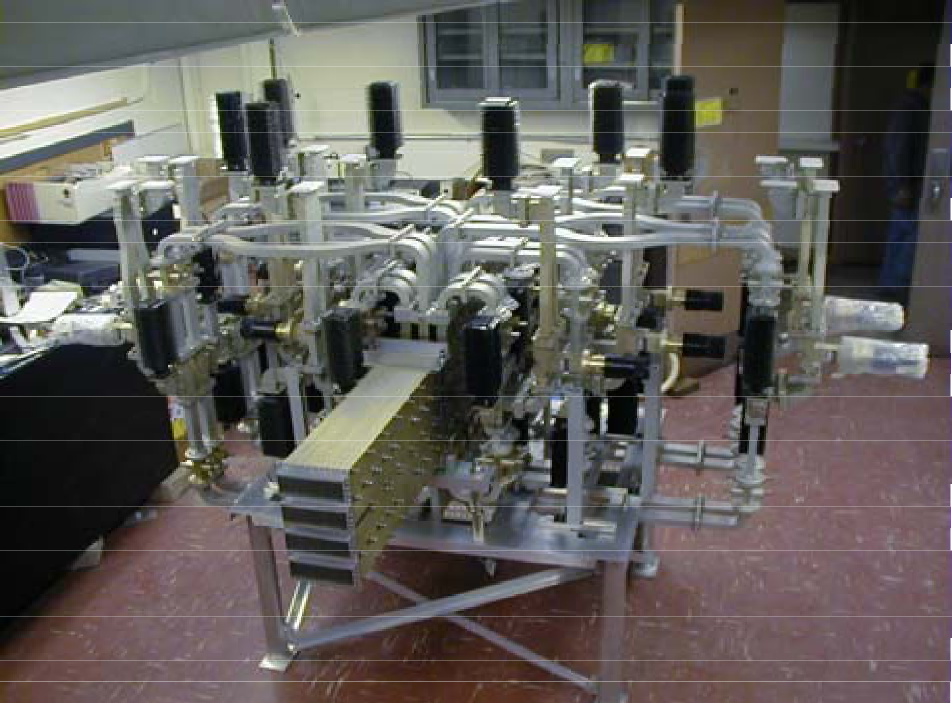
\includegraphics[width=0.7\linewidth]{figures/chap3/CMod_LH1}
	\caption{The Alcator C-Mod LH1 launcher (88 waveguides, 4.6~GHz) and it associated transmission line (aka the”jungle gym”).}
	\label{fig:cmodlh1}
\end{figure}


Brambilla developed the theory of the Slow-wave coupling of a simplified grill structure to a large toroidal plasma \sidecite{brambilla1979} and applied (and still) to many different geometries, from single waveguide to hundred of waveguides array. This coupling theory has been generalized later to the Fast-wave coupling \sidecite{theilhaber1980} and to 3D rectangular waveguides in \sidecite[+1cm]{Bers1981, bers1983}. 

Qimilarly to ICRF antennas, the wave excited by LHRF antenna is evanescent if the electron density is below a cut-off density $n_c$ (Eq.(\ref{eq:lh_cutoff_density})). However, if such a low density layer is thin enough, the wave can tunnel through it. Thus, the LH launcher must be close enough of the plasma in order to efficiently couple high power. 

In these conditions, the thermal and mechanical stresses are essential parameters to design an LH launcher. They and constitute a challenge to deliver such for these systems in for fusion reactors. As for IC antennas, LHCD launchers distributed in the vacuum vessel is being proposed for DEMO, mitigating substantially these issues \sidecite{bosia2014, kim2019}. 

% #####################################################
% #####################################################
\subsection{Multijunction Launchers}\label{sec:multijunction}
\begin{marginfigure}
	\centering
	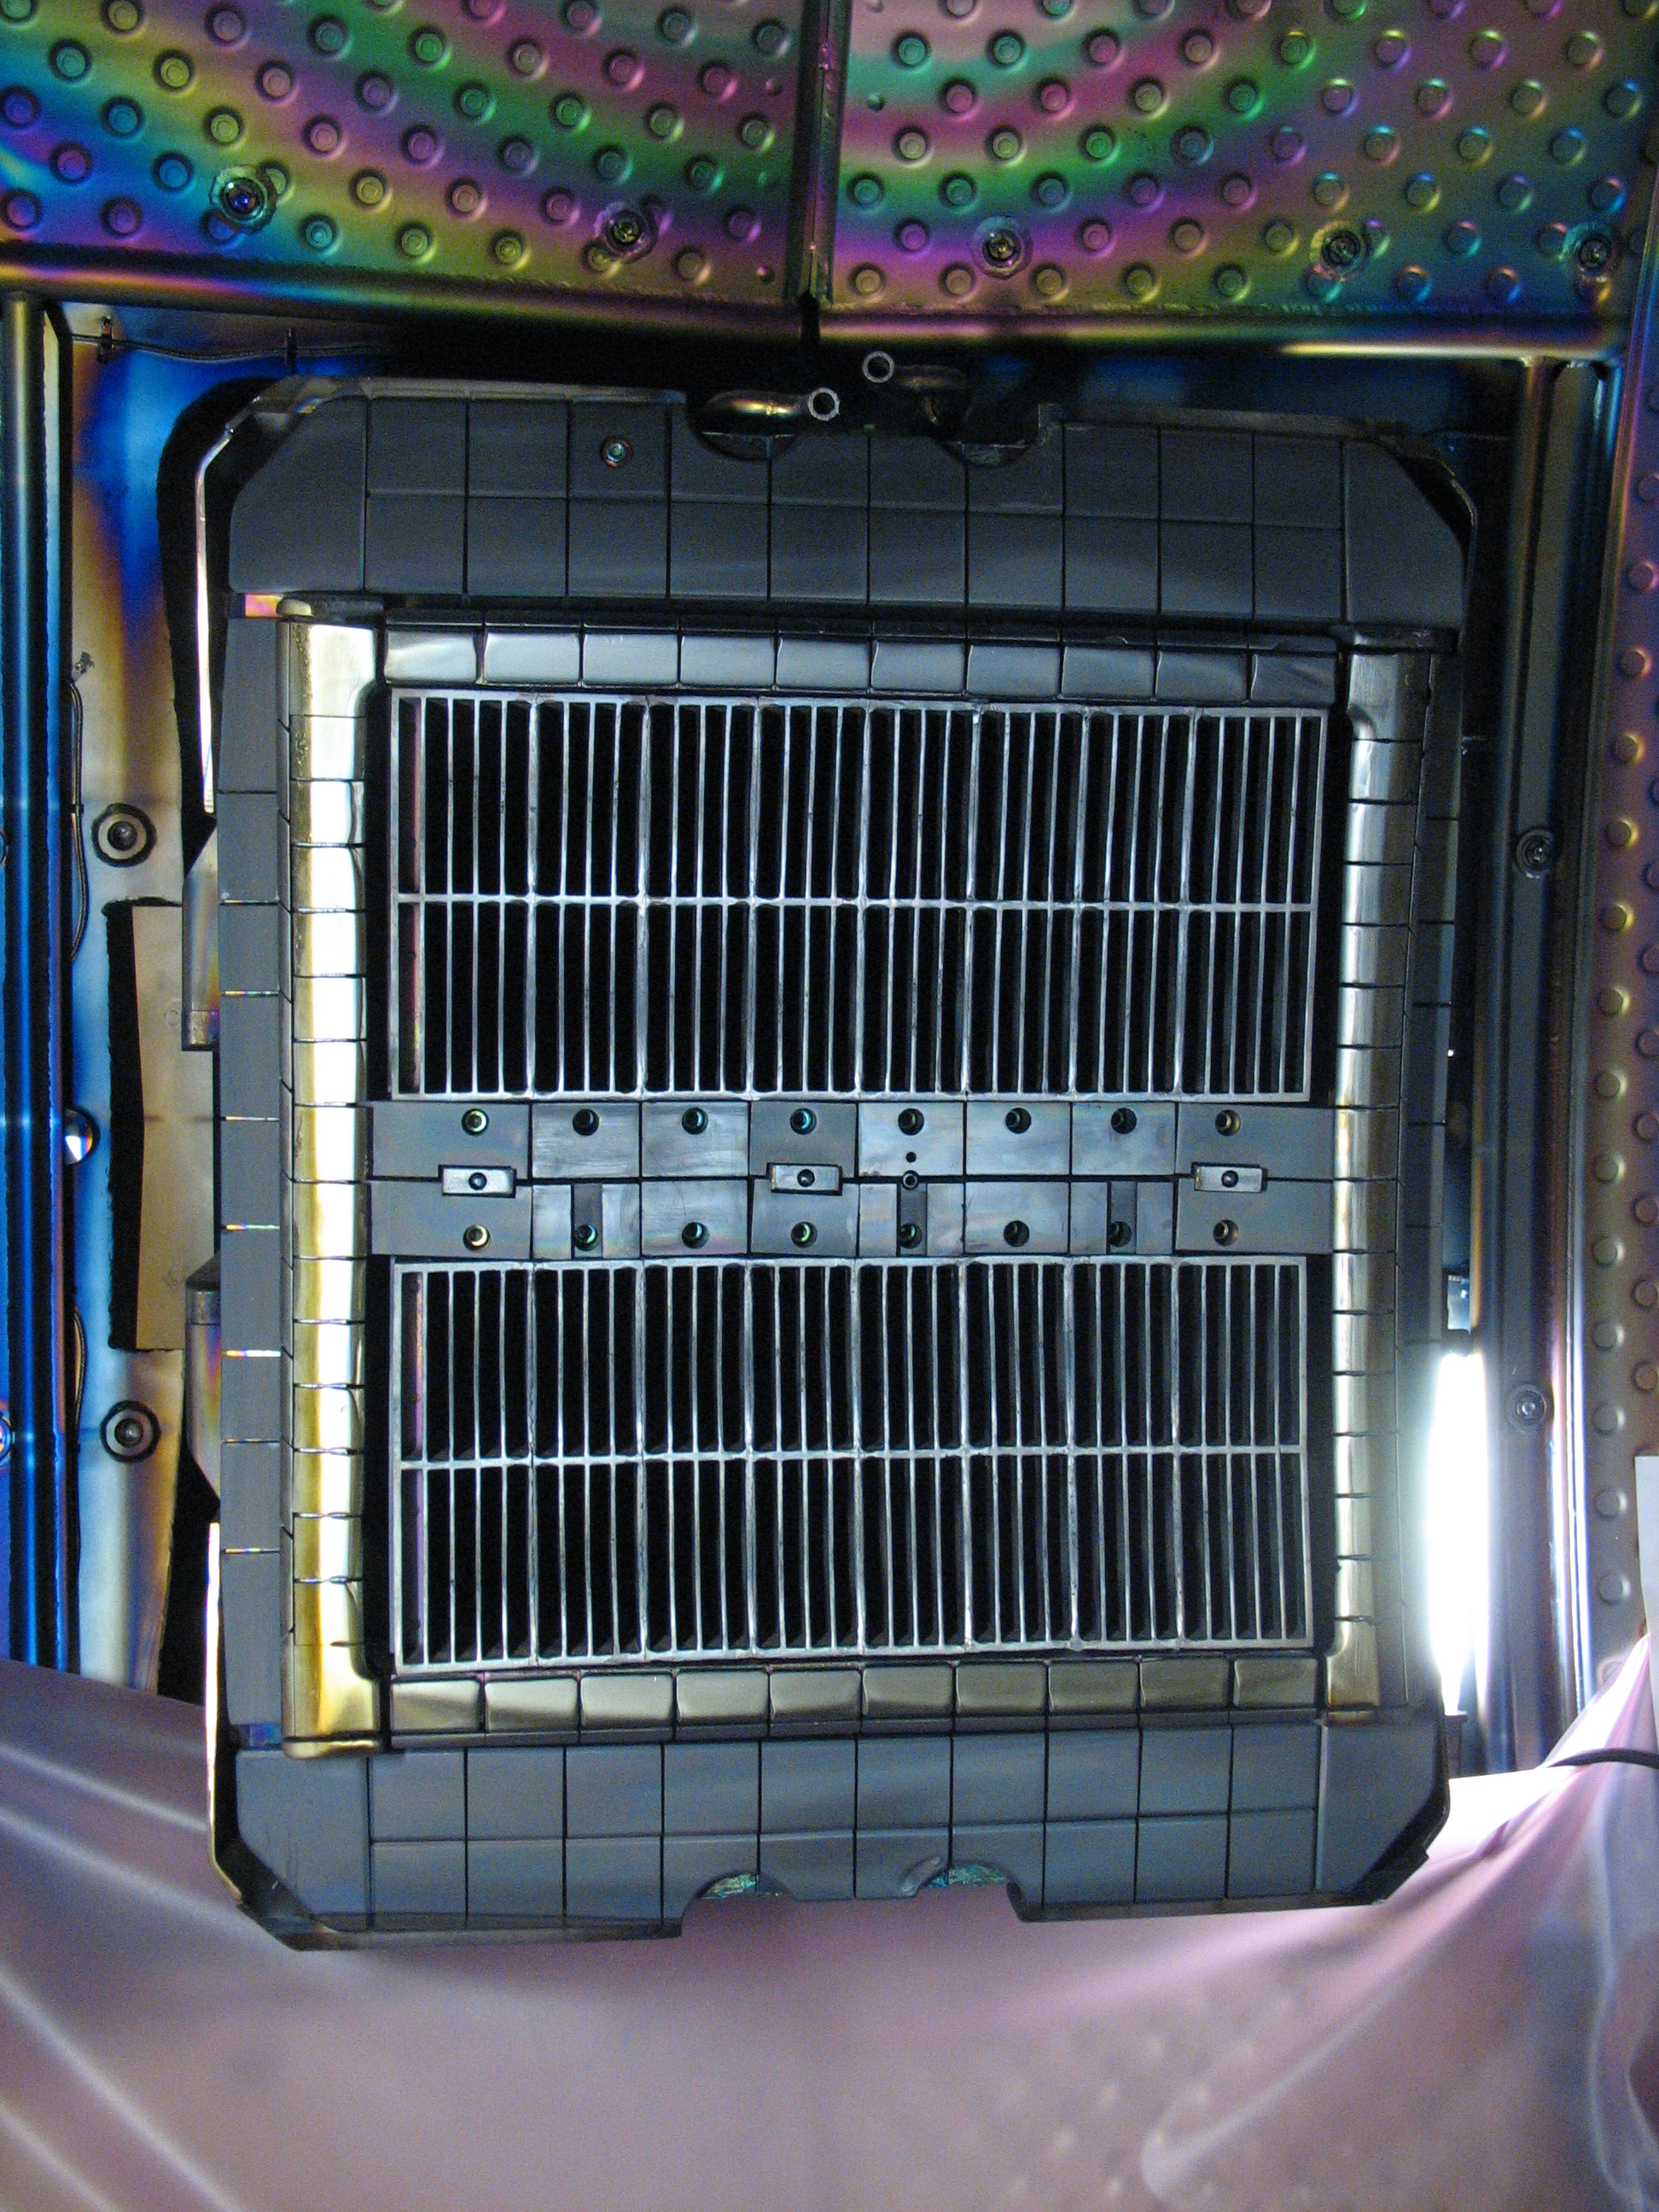
\includegraphics[width=0.9\linewidth]{figures/chap3/ToreSupra_C2}
	\caption{Tore Supra Multijunction launcher C2 as view from inside the vacuum vessel. (128 waveguides, total dimensions 50 x 40 cm, 1989). Frequency: 3.7GHz.}
	\label{fig:toresupraC2}
\end{marginfigure}
In a large tokamak, a conventional LH grill made of independently fed waveguides would require hundred of waveguides, leading to a very complex power splitting design behind the antenna (cf.Figure \ref{fig:cmodlh1}). The use of \emph{multijunction} grill was suggested in \citeauthyear{gormezano1985} to overcome this limitation. In a multijunction grill, the main waveguide is divided into $N$ smaller (secondary waveguides) by thin metallic walls parallels to the wall of the main waveguide and perpendicular to the electric field: the \emph{E-plane N-junctions}. Built-in phase shifters made by reducing the waveguide height (in order to increase the guided wave phase velocity) are added in the structure in order to obtain the desired output phasing of the grill. Multijunction launcher makes it simpler to create and feed a large number or waveguides, at the contrary of classic grills launchers. However, a drawback is that the adjustment range of the power density spectrum is limited to a smaller range than for classic grills launchers.

\begin{marginfigure}
	\centering
	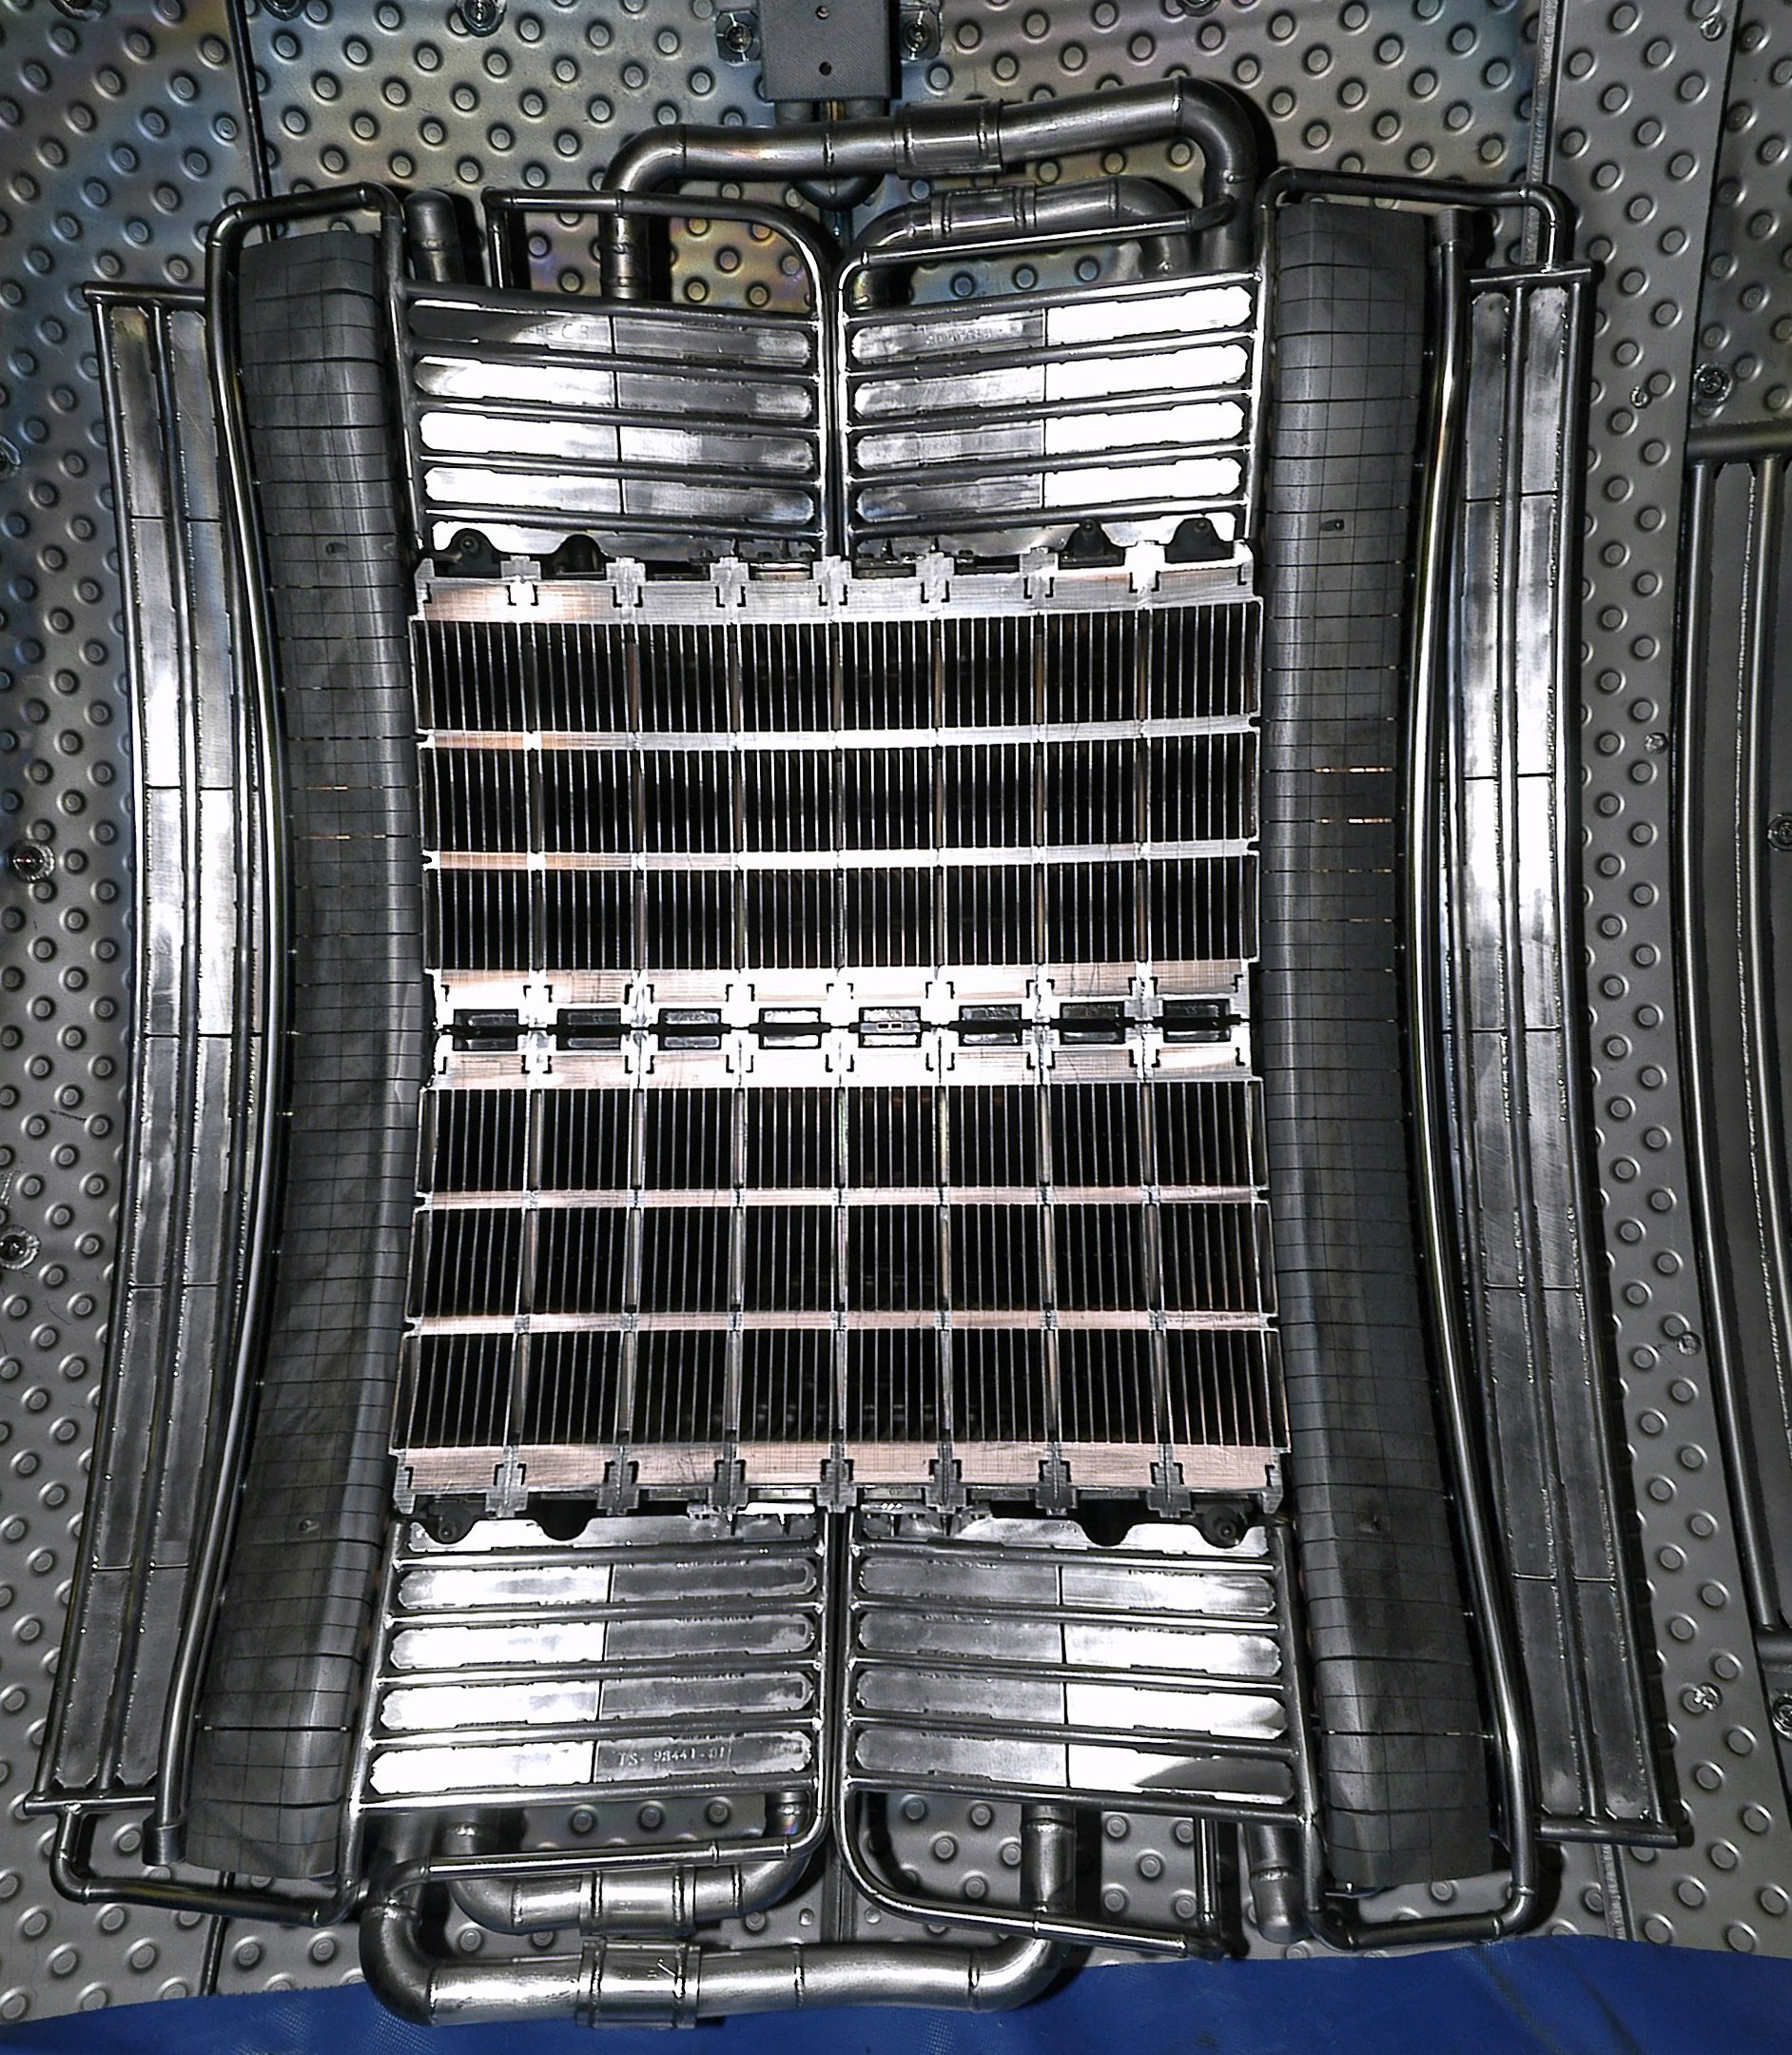
\includegraphics[width=0.9\linewidth]{figures/chap3/ToreSupra_C3}
	\caption{Tore Supra Multijunction launcher C3 (now LH1 in WEST) (288 waveguides, total dimensions 60cm x 60cm, 1999). Frequency: 3.7GHz.}
	\label{fig:toresupraC3}
\end{marginfigure}

A judicious choice of the phasing of the output waveguides leads to an important self-matching property of the multijunction (also known as \emph{recycling effect} or \emph{load resilience}). Indeed, for specific phase values, the reflected waves from the plasma which return back in the secondary waveguides can be reflected back to the plasma, thus leading to multiple reflections in the secondary waveguides. This recycling effect, which takes place between the plasma-antenna discontinuity and the E-plane bi-junctions, leads to an attenuation of the waves at each passage by the plasma, and ultimately to a decrease of the reflected power toward the RF sources. 

The Tore Supra antenna C1 and C2 (Figure~\ref{fig:toresupraC2}), then C3 (Figure~\ref{fig:toresupraC3}) (now named LH1 in WEST) are multijunction antennas.

%\todo{Illustration of the recycling effect (load resilience) inside a multijunction}.



% #####################################################
\subsection{Passive-Active waveguide array launchers}
\begin{marginfigure}
	\centering
	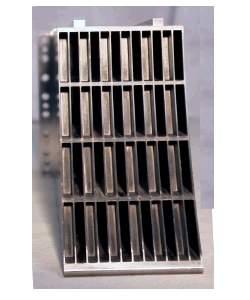
\includegraphics[width=0.8\linewidth]{figures/chap3/Pam_FTU}
	\caption{PAM prototype tested on the FTU tokamak (24 active waveguides, 24 passive waveguides, 8 GHz, 2003) \cite{mirizzi2003, ridolfini2005}.}
	\label{fig:pamftu}
\end{marginfigure}
One of the main show-stopper to the use of LHCD to realize long and efficient pulses (outside the constraints of the tokamak magnetic coils heating) is the ability to couple high LH power to the plasma. Indeed, in order to achieve good coupling, the electron density in front of the LH launchers needs to be large enough, which means that the launcher needs to be located close enough to the plasma or to increase the local density by gas puffing means. 

The alternation of \emph{passive} waveguide (a waveguide closed by a short-circuit) and \emph{active} waveguide (a waveguide that is directly fed from the generator) has been initially proposed by \citeauthyear{motley1980} in order to minimize the \emph{surface wave} excitation. Moreover, it was found that adding passive waveguide at each side of the array leads to decrease the reflected power in the last active guide \sidecite{krapchev1978, motley1980}. The passive waveguides act as reflectors, radiating back a part of the power reflected by the plasma, and thus improving the coupling efficiency. Passive-Active grills were envisaged since the 1980' for fusion-reactor grade devices \sidecite{ehst1982}. In these first conceptual designs, the passive waveguides were thought to be plugged or tuned individually in order for the outgoing power to have the requisite phase corresponding to an all-active grill system. 

Being close to the plasma leads to increase the heat fluxes into on the launcher front face. Thus, in order to improve the cooling of the launcher front face, it has been proposed in \citeauthyear{bibet1995} to insert one passive waveguide between each active waveguide, behind which a water pipe could efficiently water-cool the structure. 

\begin{marginfigure}
	\centering
	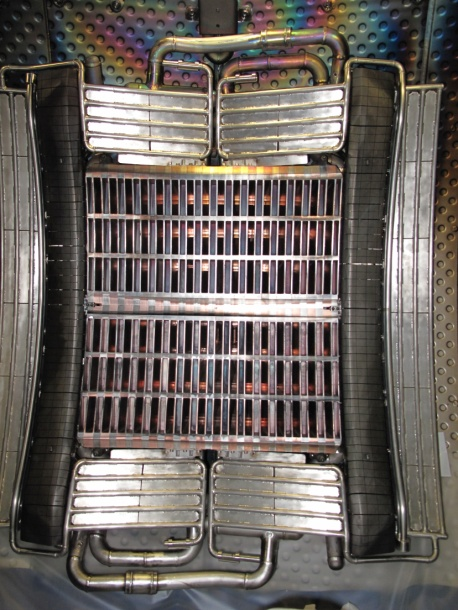
\includegraphics[width=0.9\linewidth]{figures/chap3/ToreSupra_C4}
	\caption{The Tore Supra PAM (C4, now named LH2 in WEST) launcher. (96 active waveguides, 102 passive waveguides, approx. 7 tons, front face dimensions 60cm x 60cm, 3.7 GHz, 2009).}
	\label{fig:toresuprac4}
\end{marginfigure}
In order to insure a lower reflected power than a conventional grill, it has been proposed to associate this alternation of passive-active waveguide to  use a multijunction. This is the \textit{Passive-Active Multijunction} (PAM) concept, which addresses two of the main criticisms made to LH launchers, i.e. the coupling efficiency and the heat loads resilience. The WEST Antenna LH2 (previously named C4 in Tore Supra) is a PAM antenna (Figure~\ref{fig:toresuprac4}, \citeauthyear{guilhem2009, guilhem2011}). 


% #####################################################
% #####################################################
\subsection{Poloidal splitter launchers}
\begin{marginfigure}
	\centering
	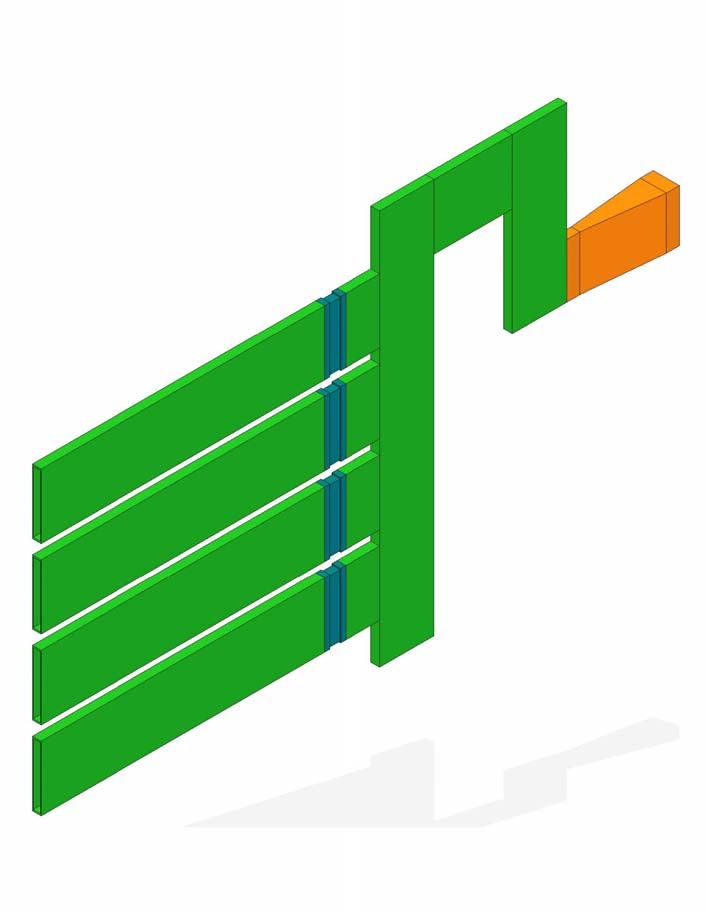
\includegraphics[width=0.8\linewidth]{figures/chap3/FourWaySplitter_1module}
	\caption{CAD conceptual schematics of the four-way splitter of Alcator C-Mod (\citeauthyear{koert2009})}
	\label{fig:fourwaysplitter1module}
\end{marginfigure}

Motivated by the reduction of the RF losses and the increase of the reliability of a LH launcher, while keeping the flexibility in the parallel index $n_{\parallel}$ spectrum of the “grill” configuration (at the contrary of multijunction), the Alcator C-Mod team developed in 2008 a launcher (LH2) based on a four way splitter \sidecite[-2cm]{koert2009}. At the contrary of multijunction launcher, the four way splitter divides the power in the poloidal direction. Since the power splitting is done poloidally, the launched parallel power spectrum can be changed with the same flexibility as with conventional grill antennas. This design simplified the feeding structure of the antenna, thus reducing the RF losses due to multiple power splitters and flanges of previous grill configurations, while keeping a simple manufacturing assembly. The RF power is redistributed depending on the plasma load on each of the four rows of the splitter. If the load is the same for each row, the power is evenly split among rows. The RF optimization of the launcher has been made for a source frequency of 4.6 GHz and assuming a simplified plasma load (constant) in front of each row. A similar design has been made for the KSTAR tokamak, at 5~GHz \sidecite[-1cm]{kim2012, kim2019}. 


\begin{figure}[h]
	\centering
	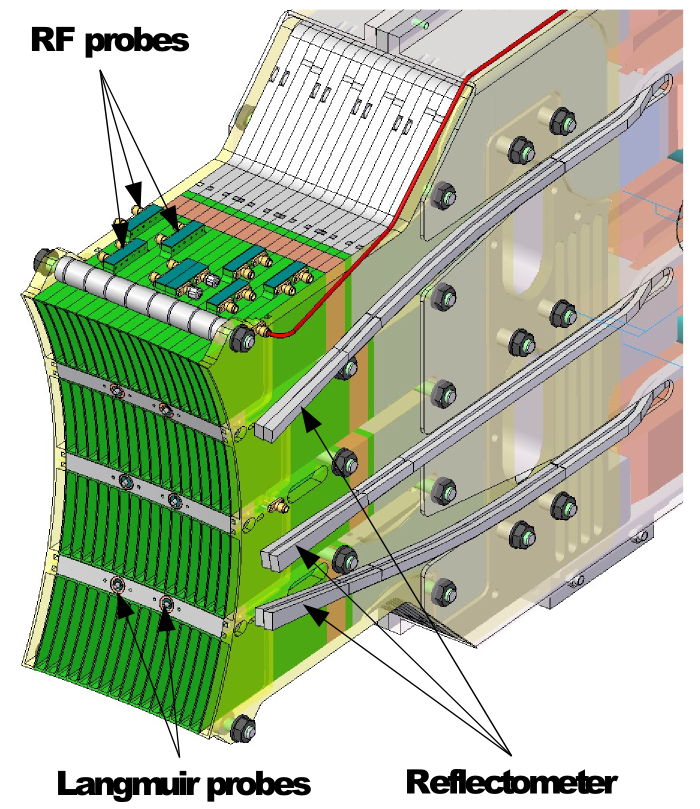
\includegraphics[width=0.4\linewidth]{figures/chap3/FourWaySplitter_CAD}
	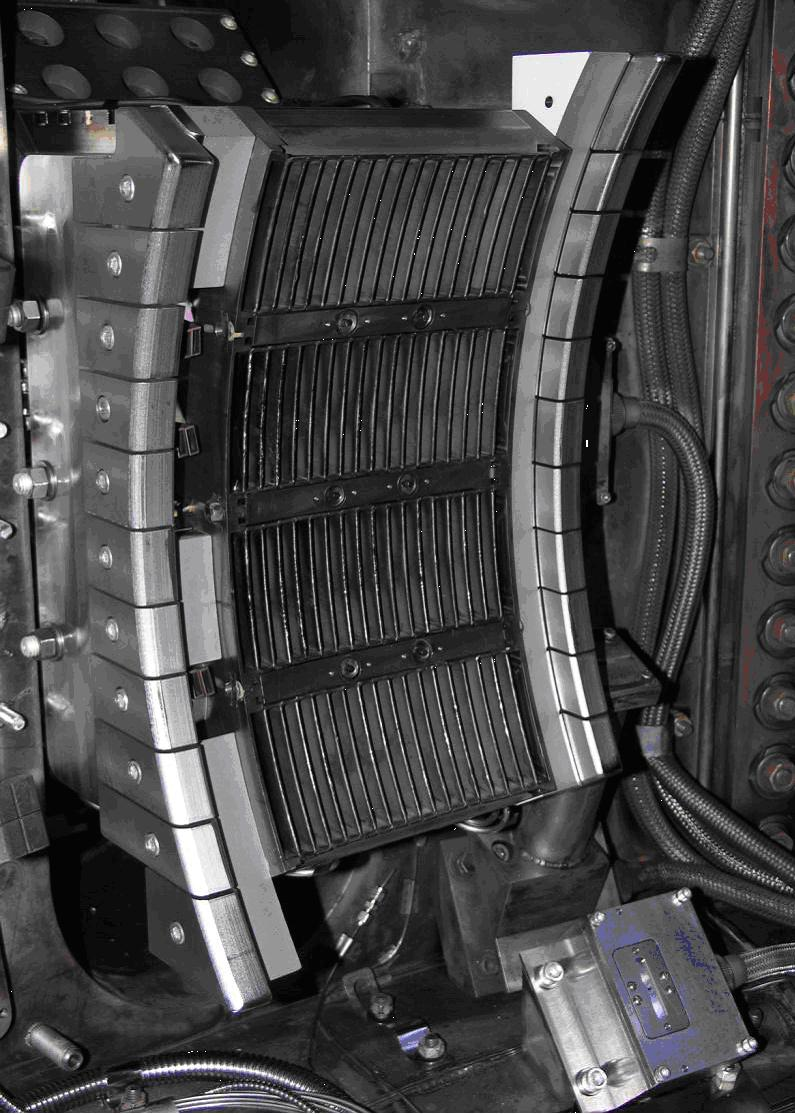
\includegraphics[width=0.35\linewidth]{figures/chap3/CMod_LH2}
	\caption{Left: final assembly CAD model with 16 four-way splitters. Right: Picture of the LH2 launcher inside the Alcator C-Mod vacuum vessel with its lateral protections in January 2012 (\citeauthyear{Meneghini2012}).}
	\label{fig:cmodlh2}
\end{figure}

%
%
%% #####################################################
%\subsection{LH systems and launchers performances}
%Mainly because of its relative simplicity, most of the LH launchers have been based on a "grill" configuration, as for example in the 1980' \sidecite{porkolab1984, gormezano1986, stevens1988}.
%
%Typical grill launchers have a high reflection coefficient (of the order of 20 to 40\%) but directivity higher than 80\%. Since all the waveguides can be feed by independent RF sources, and thus independently phased, such launchers have a wide flexibility in terms of operational space (excited spectrum) which is of great interest for physics studies. However, since each waveguide is independently power fed, the complexity of the launcher grows enormously with the number of output waveguides, leading to cumbersome transmission systems for multi-megawatt power levels (Table \ref{tab:grillperformances}). 
%
%\begin{table}
%	{\rowcolors{2}{Apricot}{Dandelion}
%		\begin{tabular}{| p{6cm} | p{5cm} |}
%			\hline 
%			Launcher & Total number of waveguides \\
%			\hline \hline
%			PLT Grill 1 (1981-1984)  \sidecite{stevens1988} & 6 (0.8 GHz) \\
%			\hline
%			PLT Grill 4 (1986) \sidecite{stevens1988} & 16 (2.45 GHz) \\
%			\hline
%			COMPASS-D (1989) & 8 (1.3 GHz) \\
%			\hline
%			Alcator C \sidecite{porkolab1984} & 16 (4.6 GHz) \\
%			\hline
%			Alcator C-Mod LH1 (2006) & 88 (4.6 GHz) \\
%			\hline
%		\end{tabular}
%	}
%	\caption{Waveguide number and maximum performances in some grill launchers.}
%	\label{tab:grillperformances}
%\end{table}
%
%Multijunction launchers at the contrary have led to hundred of waveguides launchers (see Table \ref{tab:multijunctionperformances}). The complexity of the multijunction design and manufacturing is balanced by the a simpler transmission line system behind the launcher. Because of the self-matching property, the typical reflection coefficient of multijunction launchers is generally less than 10\%. However, the multiple back and forth of the waves leads to an increase of the peak electric field in secondary waveguides. Moreover, since the phase shift is created by the built-in phase shifter inside the launcher, the flexibility of phase configuration is reduced in comparison to classic grill launchers. 
%
%\begin{table}
%	{\rowcolors{2}{Apricot}{Dandelion}
%		\begin{tabular}{| p{6cm} | p{5cm} |}
%			\hline 
%			Launcher	& Total number of waveguides  \\ 
%			\hline \hline
%			Petula-B \sidecite{gormezano1985}	& 4 (1.3 GHz)    \\ 
%			\hline 
%			JT60 CD-3 \sidecite{ikeda1989-1}	& 24x4=96 (1.74-2.23 GHz)    \\ 
%			\hline 
%			JET \sidecite{litaudon1990}	& 2x2x2x6x8=384 (3.7 GHz)   \\ 
%			\hline 
%			Tore Supra C1 and C2 \sidecite{litaudon1992}	& 4x2x8x2=128 (3.7 GHz)   \\ 
%			\hline 
%			Tore Supra C3 \sidecite{bibet2000}	& 6x3x8x2=288 (3.7 GHz)   \\ 
%			\hline 
%			EAST & 8x4x5=160 (2.45 GHz) \\
%			& (4.6 GHz) \\
%			\hline
%		\end{tabular} 
%	}
%	\caption{Waveguide number and maximum performances in some multijunction launchers}
%	\label{tab:multijunctionperformances}
%\end{table}
%
%\begin{table}
%	\begin{tabularx}{\textwidth}{|X|X|X|X|X|X|}
%		\hline
%		Tokamak	& Number of sources & Total installed power (MW) &	Frequency range (MHz) &	Number and type of antenna & 	Max. pulse Length (s) \\
%		\hline\hline
%		JET				& 24	& 15	& 3.7 	& 1 MJ	& 13  	\\
%		Tore-Supra/WEST 		& 16 	& 9		& 3.7	& 1 MJ 	& 		\\
%		&    	&  		&      	& 1 PAM 			& 390 	\\
%		Alcator C-Mod	& 8		& 2		& 4.6	& 1 grill			& 		\\
%		EAST			& 20 	& 4 	& 2.45 	& 1 grill 			& 		\\
%		& 24	& 6 	& 4.6	& 1 MJ	& 400 	\\
%		HL-2A 			& 4 	& 1.6	& 3.7	& 1 PAM 			& 		\\
%		SST-1 			& 4 	& 2		& 3.7 	& 1 grill			&	 	\\
%		KSTAR 			& 1 	& 0.5	& 5 	& 1 grill			& 		\\
%		ITER 			& 48	& 24 	& 3.7-5 & 1 PAM				& 1000 	\\
%		\hline
%	\end{tabularx}
%	\caption{LHCD systems of JET, Tore Supra/WEST, Alcator C-Mod, EAST, HL-2A, SST-1, KSTAR and ITER}
%	\label{tab:recentLHCDsystems}
%\end{table}
%
%The PAM concept tested in FTU and in the Tore Supra tokamak showed that reflected power lower than 5\% (i.e. high coupling efficiency) and continuous operations could be combined (cf. Figure \ref{fig:ts45472c4ir}) during long pulse operations. 
%
%\begin{figure}
%	\centering
%	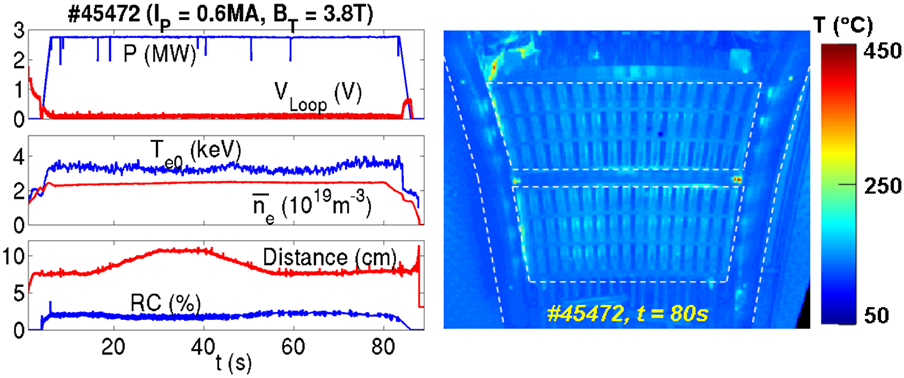
\includegraphics[width=0.9\linewidth]{figures/chap2/Tore_Supra/TS45472_C4_IR}
%	\caption{Illustration of a Tore Supra discharge with the PAM launcher (TS\#45472, 2010) \sidecite{ekedahl2010}. The design goal power density (25MW/m$^2$ ) is achieved during 78s, with very low reflected power (<2\% of the input power), even at large plasma launcher distance (~10 cm) (density is not the line-average density). The Infra-Red monitoring shows that the global temperature of the launcher mouth is lower than 270$^{\circ}$C, validating its efficient cooling structure.}
%	\label{fig:ts45472c4ir}
%\end{figure}


\clearpage
% #####################################################
% #####################################################
\section[ITER Antenna RF Design]{ITER LHCD Antenna RF Design}\label{sec:ITER_LHCD_antenna}
\marginnote{Part of this section are taken from paper \citeauthyear{hillairet2011} and \citeauthyear{hillairet2013}.}
The high current drive efficiency of lower hybrid waves makes Lower Hybrid Current Drive (LHCD) system a crucial actuator to sustain a fraction of the non-inductive current drive in tokamaks. Simulations of ITER scenarios show that LHCD can help saving the poloidal flux consumption during ramp-up phases and thus extends significantly the flat-top duration. Although not part of the initial ITER planned procurement phase, a 20~MW/CW 5~GHz LHCD system was expected to be commissioned and used for the second mission of ITER\sidenote{Since 2008, the LHCD system has been removed from the list of the heating and current drive systems of ITER\cite{iterorganization2018}.}, i.e. Q=5 steady state target. In 2011-2013, as part of an international work leaded by CEA/IRFM, CEA/IRFM made a particular R\&D effort in order to validate the design and the performances of 5~\si{GHz} LHCD system for ITER\sidecite{hoang2009-1}. 

Depending on the plasma scenarios (steady-state, hybrid, ramp-up, etc.), the additional current driven by LHCD would range between 0.42 MA (steady-state) up to more than 3.0~MA (ramp-up) \sidecite{decker2011}. In any case, these values confirm that for steady state scenarios, a substantial bootstrap current is required \sidecite{jacquinot1999}. The average current drive efficiency, which is the figure of merit of the LHCD, has been calculated to be $\eta \equiv 0.2 \times 10^{20} \si{A m^{-2} W^{-1}}$, similar to the ones measured in present days tokamaks \sidecite{jacquinot1999}. This value  can be compared to other additional current drive scheme, such as NBI or ECCD. 

On the technological aspect, the Passive Active Multijunction launcher concept has been validated on FTU\sidecite{pericoli-ridolfini1999} and in steady-state conditions at 3.7~\si{GHz} on Tore Supra (Cf. previous Section) \sidecite{ekedahl2010}. For this reason, the ITER LHCD antenna design is based on a PAM antenna. However, its scalability to 5~\si{GHz} especially in terms of high power handling and Continuous Wave (CW) operations remains to be demonstrated. 

In ITER, a main parallel index of the launched waves $n_{\parallel 0} \approx 2.0$ has been selected as a trade-off between the current drive efficiency, the wave accessibility and the location of power deposition, all of which depend upon the plasma conditions\sidecite{becoulet2011}. In frame of an international work leaded by CEA/IRFM, a new arrangement of PAM has been studied in order to allow a larger $n_{\parallel}$ flexibility compared to the previous design\cite{bibet2005-1}, i.e. increasing the peak $n_{\parallel}$ range from $\left[1.9-2.1\right]$ to $\left[1.8-2.2\right]$. 

\begin{figure}
	\centering
	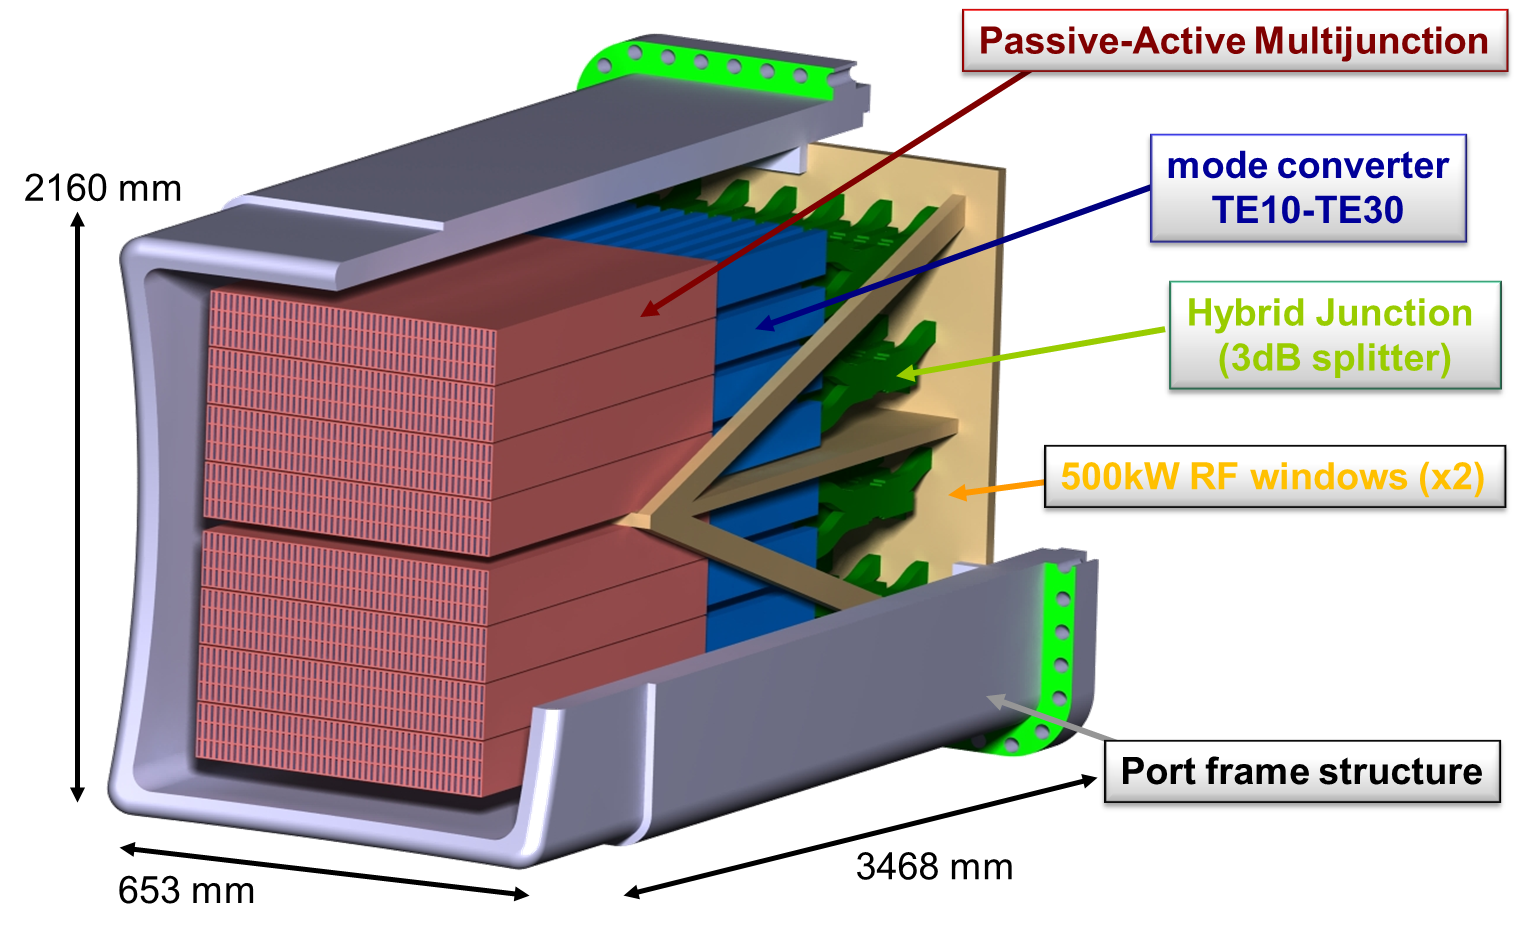
\includegraphics[width=1.0\linewidth]{figures/chap3/ITER_antenna/ITER_LH_antenna}
	\caption{Illustration of the conceptual design of the ITER LHCD antenna. }
	\label{fig:iterlhantenna}
\end{figure}

In this design, the launcher is made of 48 identical modules, each one independently fed by one klystron: twelve in the toroidal direction and four in the poloidal direction. A module consists of four active waveguides in the toroidal direction and six lines of waveguides in the poloidal direction (Figure~\ref{fig:3D-view_1module}). Thus, the whole launcher contains 1152 active waveguides whose dimensions are $9.25\times58$~mm. The RF power is carried through a transmission line up to a RF window
located inside the frame and connected to a poloidal 3~dB splitter which feeds two $\TE_{10}-\TE_{30}$ mode converters. Each of these mode converters converts the incident power from the rectangular $\TE_{10}$ mode to the rectangular $\TE_{30}$ mode in order to divides the power into three poloidal rows, corresponding to the input of a 4-active waveguides multijunction. 

\begin{figure}
	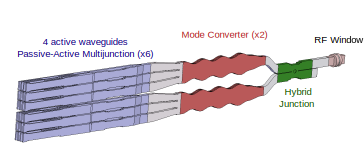
\includegraphics[width=1.0\textwidth]{figures/chap3/ITER_antenna/LH4ITER_1module}
	\caption{3D view of one module (RF modelling): the power is coming from the
		right of the figure, through the RF window, the hybrid junction, the
		two mode converters and the six PAM multijunctions. All the elements
		of a module located behind the RF window are under the machine vacuum.}
	\label{fig:3D-view_1module}
\end{figure}

An illustration of the multijunction design, with four active waveguides per toroidal line is shown in Figure~\ref{fig:Illustration_4awg_design}. The passive waveguides, not illustrated in the Figure, are inserted between each active waveguides. In this design, the active waveguides (of width $b_{a}=9.25$~mm) are wider then passive waveguides ($b_{p}=7.25$~mm). The waveguides height ($a=58$~mm) avoids the higher mode $\TE_{20}$ to propagate and is close to the WR229 standard ($58.17\times29.08$~mm). 

The structure has been optimized in order to reach the following goals: i) minimize the reflected power, ii) insure a $270\si{\degree}$ phase shift between adjacent active waveguides. The estimated return loss of the optimized structure is $-34$~dB while the phase difference between adjacent output waveguides is $270\si{\degree} \pm 0.7\si{\degree}$. The transmitted power $\left|S_{n1}\right|^{2}$ (with $n=\{2,3,4,5\})$ is $1/4\pm7\times10^{-3}$ which means that the input power is well divided into the 4 output of the multijunction. The maximum electric field on matched ports is 346~kV/m for a power input of 250~kW, the propagation loss $1-\sum_{n} \left| S_{n1} \right|^{2}$ for copper walls is 1.2\% and the total length of the multijunction illustrated in Figure\ref{fig:Illustration_4awg_design} is $1.170$~m. 

\begin{figure}[h]
	\centering{}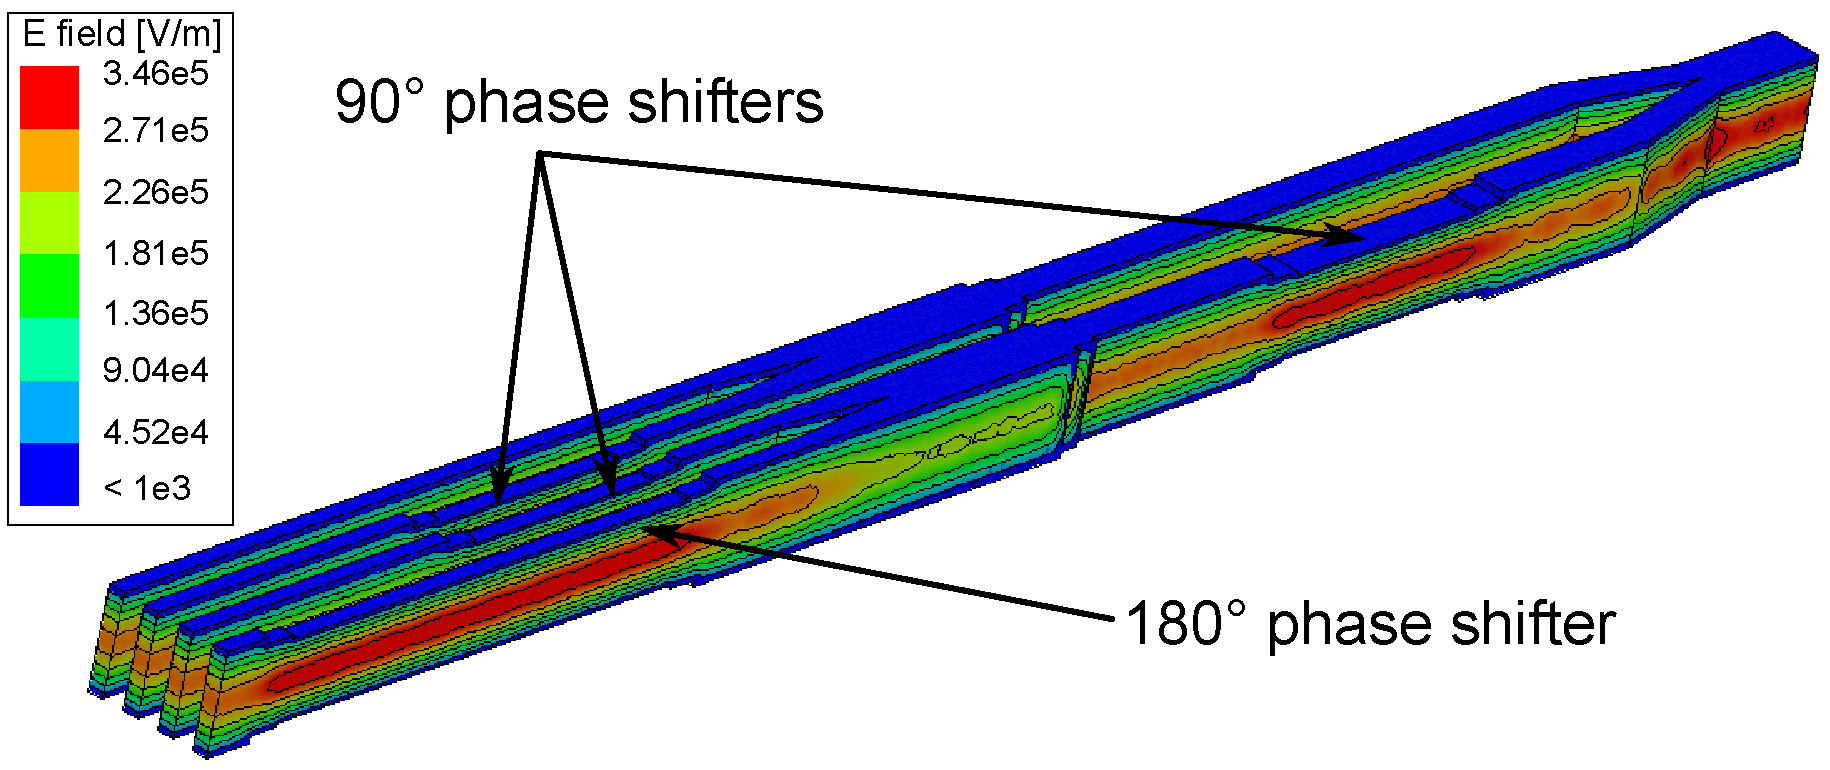
\includegraphics[width=0.9\textwidth]{figures/chap3/ITER_antenna/LH4ITER_MJ_4awg}
	\caption{Electric field into the 4 active waveguides multijunction design.
		The input power is 83~kW, corresponding to the 250~kW incoming
		into the mode converter then divided by 3 in each rows of the poloidal
		divider. The passive waveguides located between each active waveguides
		are not illustrated in this picture. 5~GHz ANSYS HFSS simulation
		on matched ports.}
	\label{fig:Illustration_4awg_design} 
\end{figure}

The waveguide phasing is provided by one 180\si{\degree} phase shifter (in the second bi-junction) and three 90\si{\degree} phase shifters. 6 identical multijunctions are used to fill one row of a module of the ITER LHCD antenna. As in the 2001 initial design, 3 multijunctions disposed in a poloidal column are fed by a $\TE_{10}-\TE_{30}$ mode converter. This mode converter is detailled in Section~\ref{sec:mode_converter}.

The plasma coupling have been calculated using the ALOHA code~\sidecite{hillairet2010} for 6 side-by-side modules, forming rows of 24 active waveguides. As a particular attention has been made on the power division in this model, thus on the reflected power due to the mechanical phase shifters. These phase shifters have been optimized in order to provide the expected relative phase shift thus to minimize the VSWR. As a result, the average reflection coefficient (Figure~\ref{fig:iterlhrc}) of this structure is lower than the 2001 version waveguide model, remaining below that 2\% over a large density range and showing that the reflected power of a multi-junction is almost as dependant to the RF structure than the edge plasma parameters.

\begin{figure}
	\centering
	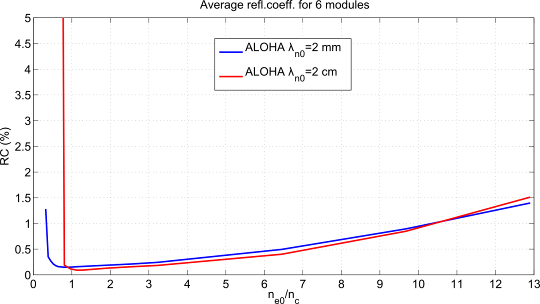
\includegraphics[width=0.9\linewidth]{figures/chap3/ITER_antenna/ITER_LH_RC}
	\caption{Average reflection coefficient versus edge electron density. The antenna is made of 6 identical modules, with 4 active waveguides per module. LH cut-off at 5GHz : nc=3.1×1017 m-3.}
	\label{fig:iterlhrc}
\end{figure}

The maximum and averaged electric fields are plotted on Figure~\ref{fig:iterlhelectricfield}. As in the 2001 design, the electric field is maximum near the cut-off density (740-800~\si{kV/m} for $n_{e0}/n_c=1$) and is in the 580-600~\si{kV/m} range for $n_{e0}/n_c=2$. Above the cut-off, the average electric field is below 300~kV/m and decreases for higher densities.

\begin{figure}
	\centering
	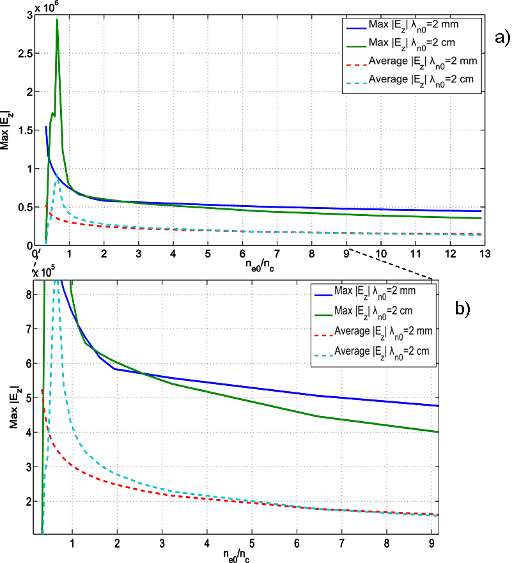
\includegraphics[width=1.0\linewidth]{figures/chap3/ITER_antenna/ITER_LH_electric_field}
	\caption{Maximum and average electric field computed by ALOHA versus edge electron density.}
	\label{fig:iterlhelectricfield}
\end{figure}



\clearpage

% #####################################################
% #####################################################
\section[ITER Mode Converter]{5 GHz ITER $\TE_{10}$-$\TE_{30}$ Mode Converter}\label{sec:mode_converter}
\marginnote{Part of this section are taken from \citeauthyear{hillairet2012, hillairet2020} and internal technical notes.}

% #####################################################
\subsection{Context}
The aim of the $\TE_{10}$-$\TE_{30}$ mode converter is to convert an input fundamental Transverse Electric (TE) rectangular mode ($\TE_{10}$) into another rectangular mode (the $\TE_{30}$ mode). This conversion is then used in order to equally split the power in three in an adapted splitter. Such splitting scheme, used in both Tore Supra LH antennas since 1999, is achieved by a perturbation of the waveguide geometry leading to mode coupling. Fundamental input $\TE_{10}$ mode can thus be almost totally converted to the $\TE_{30}$ mode, which ideally distributes the power into three in the H-plane\sidecite[-2cm]{bibet1994, wang2009}. This wall perturbation mode conversion has been used originally on ECRH, where high-order modes are not suitable for long distance transmission and plasma heating \sidecite[-1cm]{thumm1987-1, thumm2002}. 

Propagation of guided field into small perturbed wall waveguides can be modelled with the Generalized Telegraphist's equation \sidecite[-1cm]{schelkunoff1952, schelkunoff1955, unger1958, solymar1959, buckley1990}. The resulting set of equations can be solved numerically \sidecite[+0.5cm]{flugel1988,huting1989} or almost analytically with some approximations\sidecite[+2cm]{unger1958, solymar1959}. 

We refer to the previous references for more details on the calculation principles. 

% #####################################################
\subsection{RF modelling}
\subsubsection{Mode Converter}
The schematic drawing of a H-plane sinusoidal perturbated wall mode converter is illustrated in Figure \ref{fig:SchematicMC}. In Figure \ref{fig:SchematicMC}, the input $\mbox{TE}_{10}$ mode is coming from the left. Input width $a_{0}$ must be set sufficiently large in order to permit the $\TE_{30}$ mode to propagate, leading to $a_{0}\geqslant90$~mm at 5~GHz. Output width $a_{1}$ is set to insure the $\mbox{T}\mbox{E}_{50}$ mode to cut-off, i.e. $a_{1}\leqslant150$~mm. The $\mbox{TE}_{40}$ modes is able to propagate at the output width $a_{1}$, however, an incident odd TE mode upon an H-plane discontinuity
with a longitudinal symmetry only excites odd TE modes in rectangular waveguides. A similar conclusion is obtained in the case of even modes\sidenote{See \citeauthyear{dusseaux2000} and \citeauthyear{dusseaux2008} for a derivation of this property using non-orthogonal coordinates.}.  

\begin{figure}[h]
	
\includegraphics[width=0.9\textwidth]{figures/chap3/ITER_modeconverter/MC_SchematicCM}
	\caption{Schematic drawing (H-plane cut) of the $\TE_{10}-\TE_{30}$
		mode converter. }
	\label{fig:SchematicMC}
\end{figure}

The mode evolution along the mode converter is obtained by solving the generalized telegraphist's equations for a 3.5 periods deformed waveguide of wavelength $\lambda_{w}$ defined by the following sinusoidal
perturbation\cite{buckley1990, bibet1994}:

\begin{equation}
a(z)=a_{0}+\varepsilon\left(1-\cos\left(\frac{2\pi}{\lambda_{w}}z\right)\right)\label{eq:sinusoidalPerturbation}
\end{equation}
In order to reach the best mode conversion to $\TE_{30}$ mode, a numerical optimization of parameters $a_{0}$, $\varepsilon$ and $\lambda_{w}$ has been made in Matlab using a Generalized Telegraphist's equation solver. This first optimization led to dimensions $a_{0}=98$\,mm, $\varepsilon=22.4$\,mm and $k_{w}=2\pi/\lambda_{w}=36.3059\,\mbox{m}^{-1}$.

\begin{marginfigure}[-1cm]
	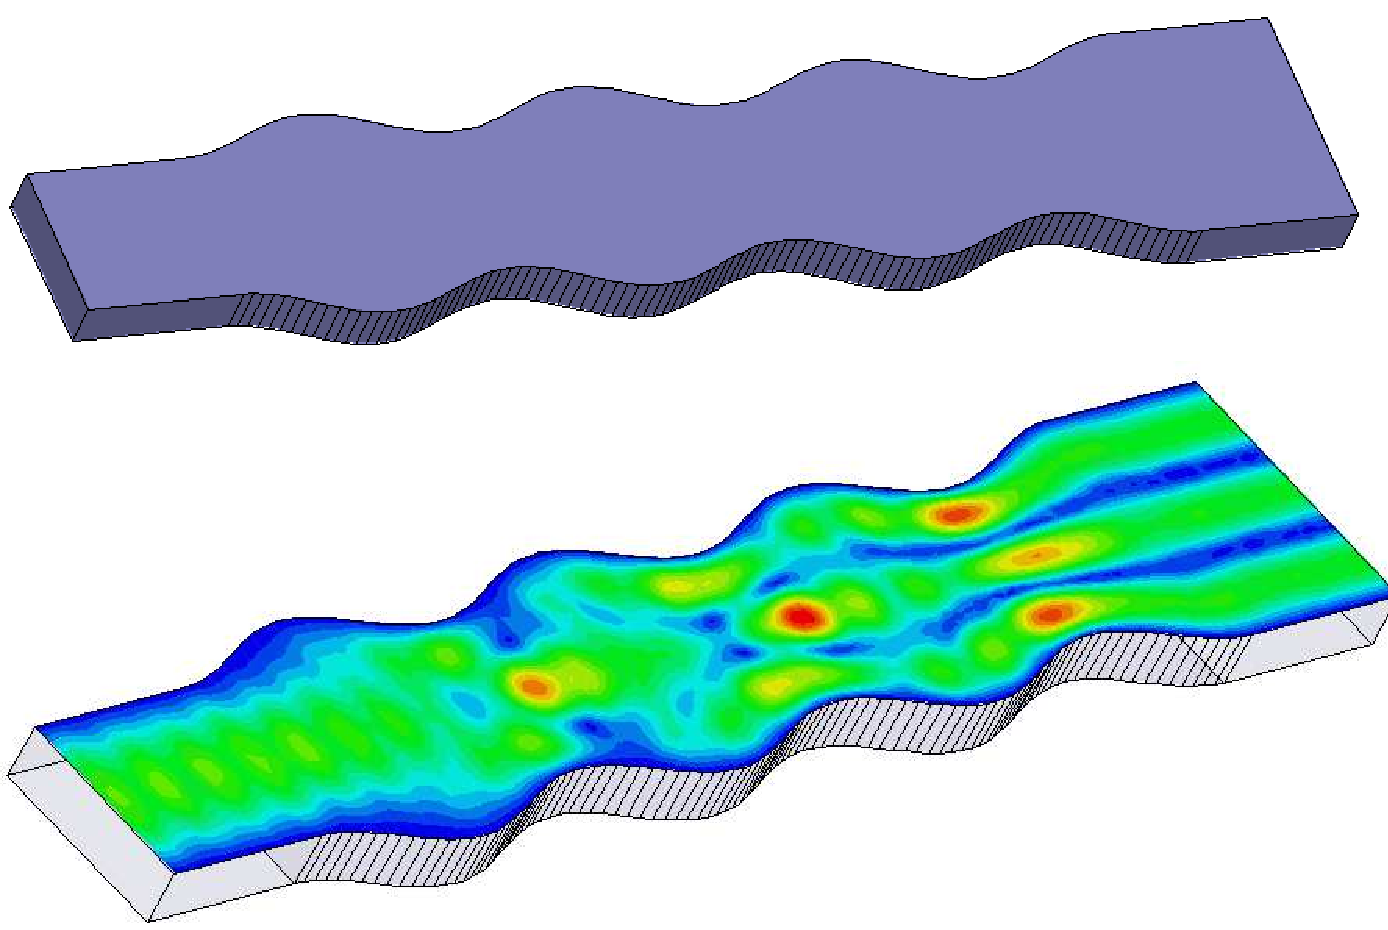
\includegraphics[width=1.0\textwidth]{figures/chap3/ITER_modeconverter/HFSS_ModeConverter}	
	\caption{HFSS RF model of the mode converter (without taper at the input).}
	\label{fig:HFSS-RF-modelMC}
\end{marginfigure}

Further optimization of these parameters have been made into ANSYS HFSS, taking into account RF conduction losses on walls. In order to avoid spurious mode generation or numerical instabilities, some extra straight rectangular waveguides have been added at the input and output of the HFSS model (Figure \ref{fig:HFSS-RF-modelMC}).  This optimization led to the dimensions reported in Table \ref{tab:DimensionsMC}, which are very close to the ones found in Matlab. 

\begin{table}[h]
	\begin{centering}
		\begin{tabular}{|c|c|}
			\hline 
			$a_{0}$ {[}mm{]} & 98\tabularnewline
			\hline 
			$\varepsilon${[}mm{]} & 22.37\tabularnewline
			\hline 
			$\lambda_{w}=\frac{2\pi}{k_{w}}${[}mm{]} & 173.06\tabularnewline
			\hline 
			$k_{w}$ {[}$\mbox{m}^{-1}${]} & 36.3059\tabularnewline
			\hline 
			$L\,(=3.5\lambda_{w})$ {[}mm{]} & 605.71\tabularnewline
			\hline 
			$a_{1}=a_{0}+2\varepsilon${[}mm{]} & 142.8\tabularnewline
			\hline 
		\end{tabular}
		\par\end{centering}
	
	\caption{Dimensions of a 5 GHz 3.5 periods $\mbox{TE}_{10}\mbox{-TE}_{30}$ mode converter.\label{tab:DimensionsMC}}
\end{table}

The return loss for the fundamental mode is 20.5~dB. Propagation losses for copper plating walls, calculated as $1-\sum_{j}\left|S_{j1}\right|^{2}$, is 1.36\%. The bandwidth of the device, defined as the range of frequencies for which at least 95\% of the $\TE_{10}$ mode is converted to $\TE_{30}$, is 120~MHz.
The length of the device is, without taking into account input and output straight rectangular waveguides, 606~mm.


In order to feed the mode converter with a standard WR-229 waveguide ($a=58.17$~mm, $b=29.08$~mm), 
an input taper has to be added to match the WR-229 width. This taper is described in the next section.

% #####################################################
\subsubsection{Input Taper}
\begin{marginfigure}
	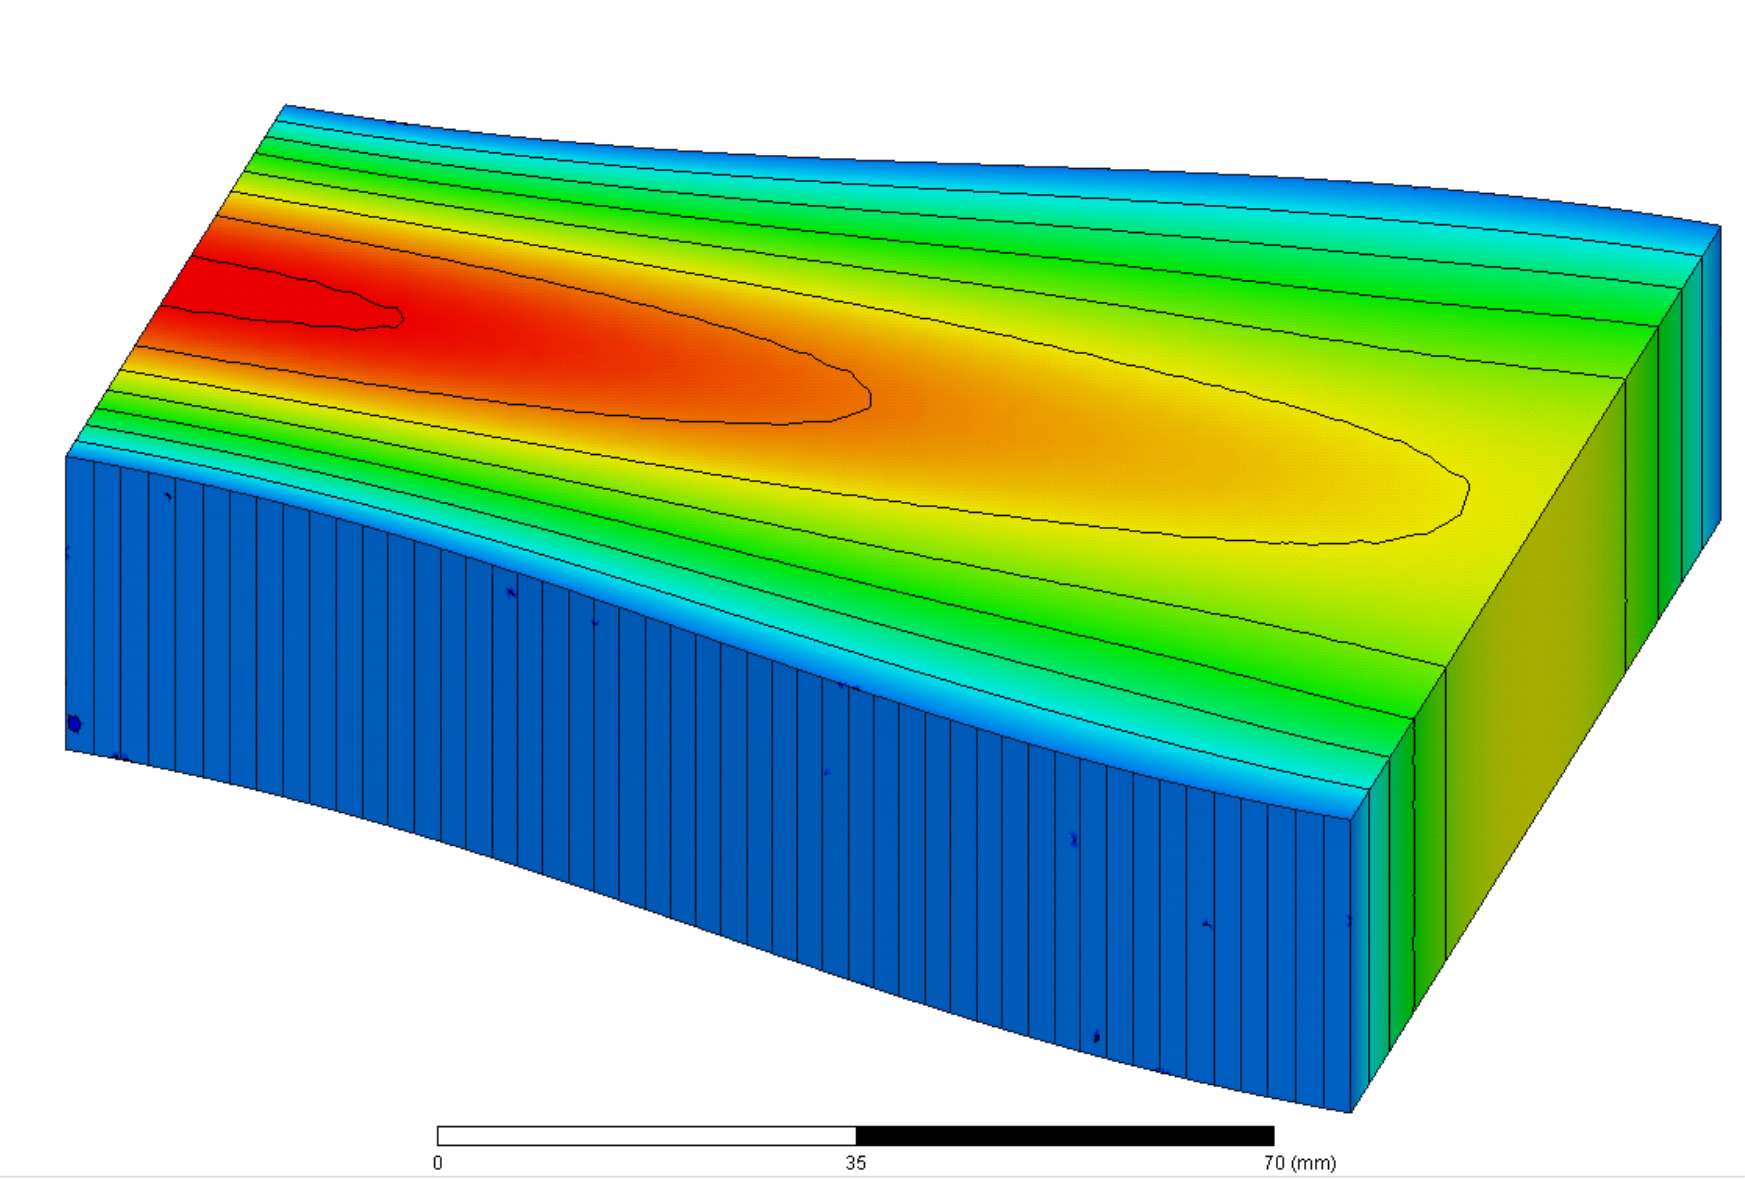
\includegraphics[width=1.0\textwidth]{figures/chap3/ITER_modeconverter/HFSS_ModeConverterTaper}
	\caption{RF Model of the Input Taper. }
	\label{fig:taper}
\end{marginfigure}
In order to make the transition between the input width $a_{0}$ of the mode converter and the conventional waveguide WR-229 width which is 58~mm, an extra taper must be added at the input (instead of the straight rectangular waveguide used before). A cosine taper has been modelled with the following width equation:
\begin{equation}
a(z)=\frac{1}{2} 
\left(a_{\mbox{WR229}}+a_{0}\right)
+\frac{1}{2}\left(a_{\mbox{WR229}}+a_{0}\right)
\cos\left[\left(\frac{z}{L_{taper}}-1\right)\pi\right]
\end{equation}
where $L_{\mbox{taper}}$ is the total length of the taper, $a_{\mbox{WR229}}$ is the WR-229 width (58.17\,mm) and $a_{0}$ the input width of the mode converter. The model has been drawn in ANSYS HFSS and then optimized in combination with mode converter. Scattering parameters are reported in Table \ref{tab:S-ParametersALL}. Let us define the forward mode conversion efficiency as the ratio between the power carried by the $\TE_{30}$ over the total forward power. According to the S-parameters, the theoretical mode conversion efficiency is close of 99.5\%. 

\begin{table}[h]
	\begin{centering}
		\begin{tabular}{|c|c|c|}
			\hline 
			Parameter & \multicolumn{1}{c|}{5 GHz HFSS } & 3.7 GHz (Tore Supra C4) \tabularnewline
			\hline 
			\hline 
			$S_{11}$$\mbox{TE}_{10}$  & -20.5 dB  & -17.7 dB\tabularnewline
			\hline 
			$S_{21}$$\mbox{TE}_{10}$ & -23 dB  & -33.6 dB\tabularnewline
			\hline 
			$S_{21}$$\mbox{TE}_{20}$ & -69.1 dB  & -81.9 dB\tabularnewline
			\hline 
			$S_{21}$$\mbox{TE}_{30}$ & -0.064 dB  & -0.0935 dB\tabularnewline
			\hline 
			Length {[}mm{]} & \multicolumn{1}{c|}{725.7} & 944\tabularnewline
			\hline 
			Max. E-field {[}kV/cm{]} & \multicolumn{1}{c|}{6.9 } & 5.8\tabularnewline
			\hline 
		\end{tabular}
		\par\end{centering}
	
	\caption{Scattering parameters of the Cosine Taper + Mode Converter (HFSS). For comparison purpose, Tore Supra mode converter results are reported. Maximum electric field has been calculated for $P_{in}=250$\,kW.\label{tab:S-ParametersALL}}
\end{table}


% #####################################################
\subsubsection{Poloidal splitter}
\begin{marginfigure}
	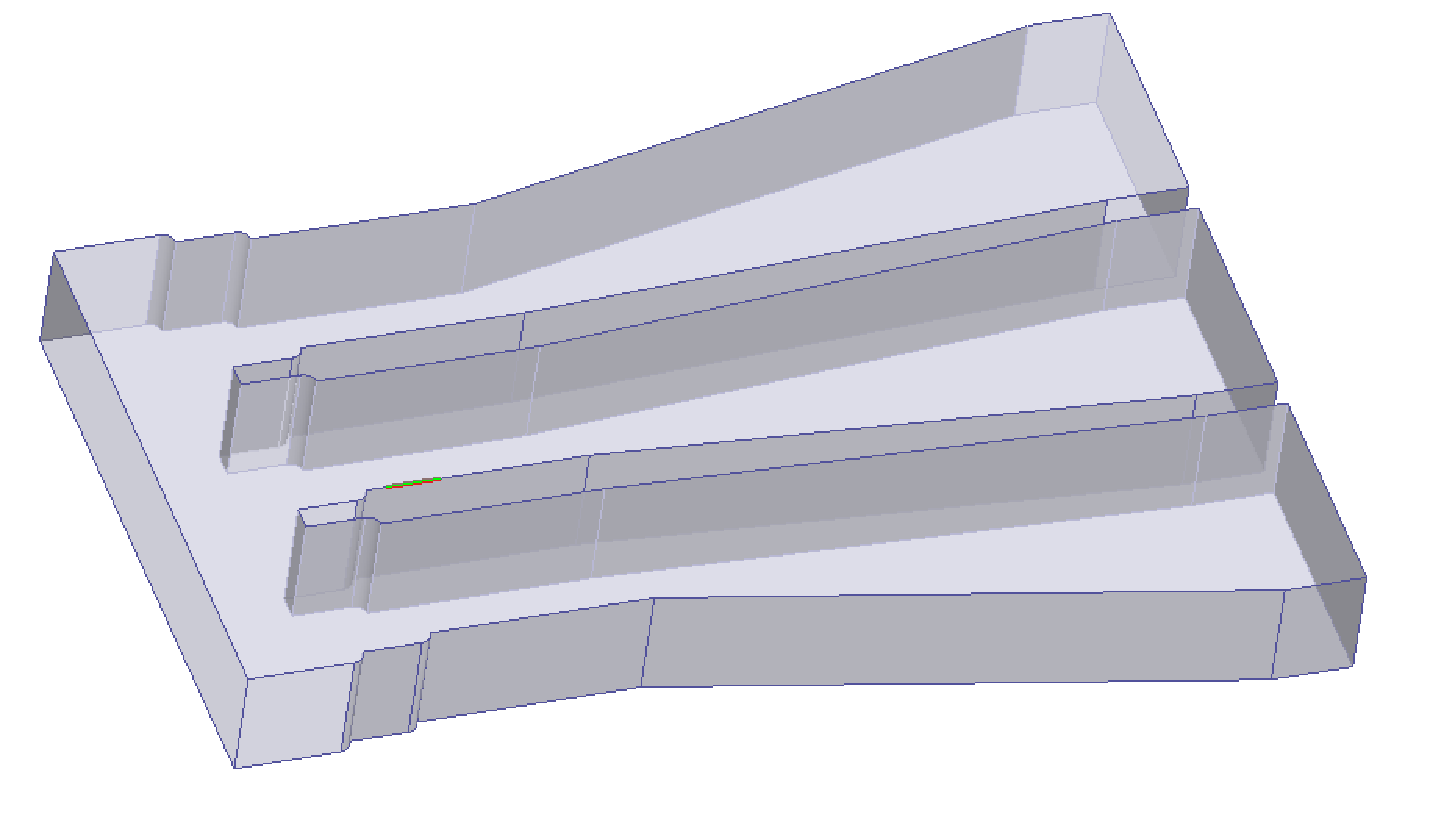
\includegraphics[width=1.0\textwidth]{figures/chap3/ITER_modeconverter/HFSS_PoloidalJunction}
	\caption{RF CAD of the poloidal splitter.}
	\label{fig:PoloidalSplitterCAD}
\end{marginfigure}
The poloidal splitter aims to split the power coming from the mode converter, which is mainly a pure $\mbox{TE}_{30}$ mode, into three distinct waveguide sections. This poloidal divider is illustrated in Figure \ref{fig:PoloidalSplitterCAD}. It has been optimized first alone in order to maximize the power splitting when exciting with a $\mbox{TE}_{30}$ mode, then with the mode converter fastened. The calculated scattering parameters of this device are reported in Table \ref{tab:PoloidalSplitter_Sparameters}.

\begin{table}[h]
	\centering{}%
	\begin{tabular}{|c|c|}
		\hline 
		Parameter & 5 GHz HFSS\tabularnewline
		\hline 
		\hline 
		$S_{11}$ for $\mbox{TE}_{30}$ & -46.3 dB\tabularnewline
		\hline 
		$S_{i1}$ for $\mbox{TE}_{30}$ & -4.81 dB\tabularnewline
		\hline 
	\end{tabular}
	\caption{Scattering parameters of the poloidal splitter.}
	\label{tab:PoloidalSplitter_Sparameters}
\end{table}

\subsubsection{Complete assembly}
The complete assembly, i.e. the mode converter associated to its input taper and the poloidal splitter has  a calculated return loss is 45.5~dB. The transmission losses are 4.79~dB $\pm$~0.01~dB for the three ports, close to the ideal value 4.77~dB which corresponding to the third of the input power. The scattering parameters evolution on a 4.9-5.1~GHz frequency band are reported in the next section.

\subsection{Low Power RF Measurements}
A low power mock-up of this 5~GHz mode converter (with its input taper) has been manufactured at CEA/IRFM using a 2-axis numerical drilling machine in Aluminum directly from the CAD model. The poloidal splitter as well as some other waveguide elements used only for measurement purposes, such as the "pull-over" described in the next section, have been manufactured by the SUMIX company from CAD models. The top of each elements has been screw tight in order to insure a very good RF contact (Figure~\ref{fig:ModeConverterMockUpElements}). 

\begin{figure}[h]
	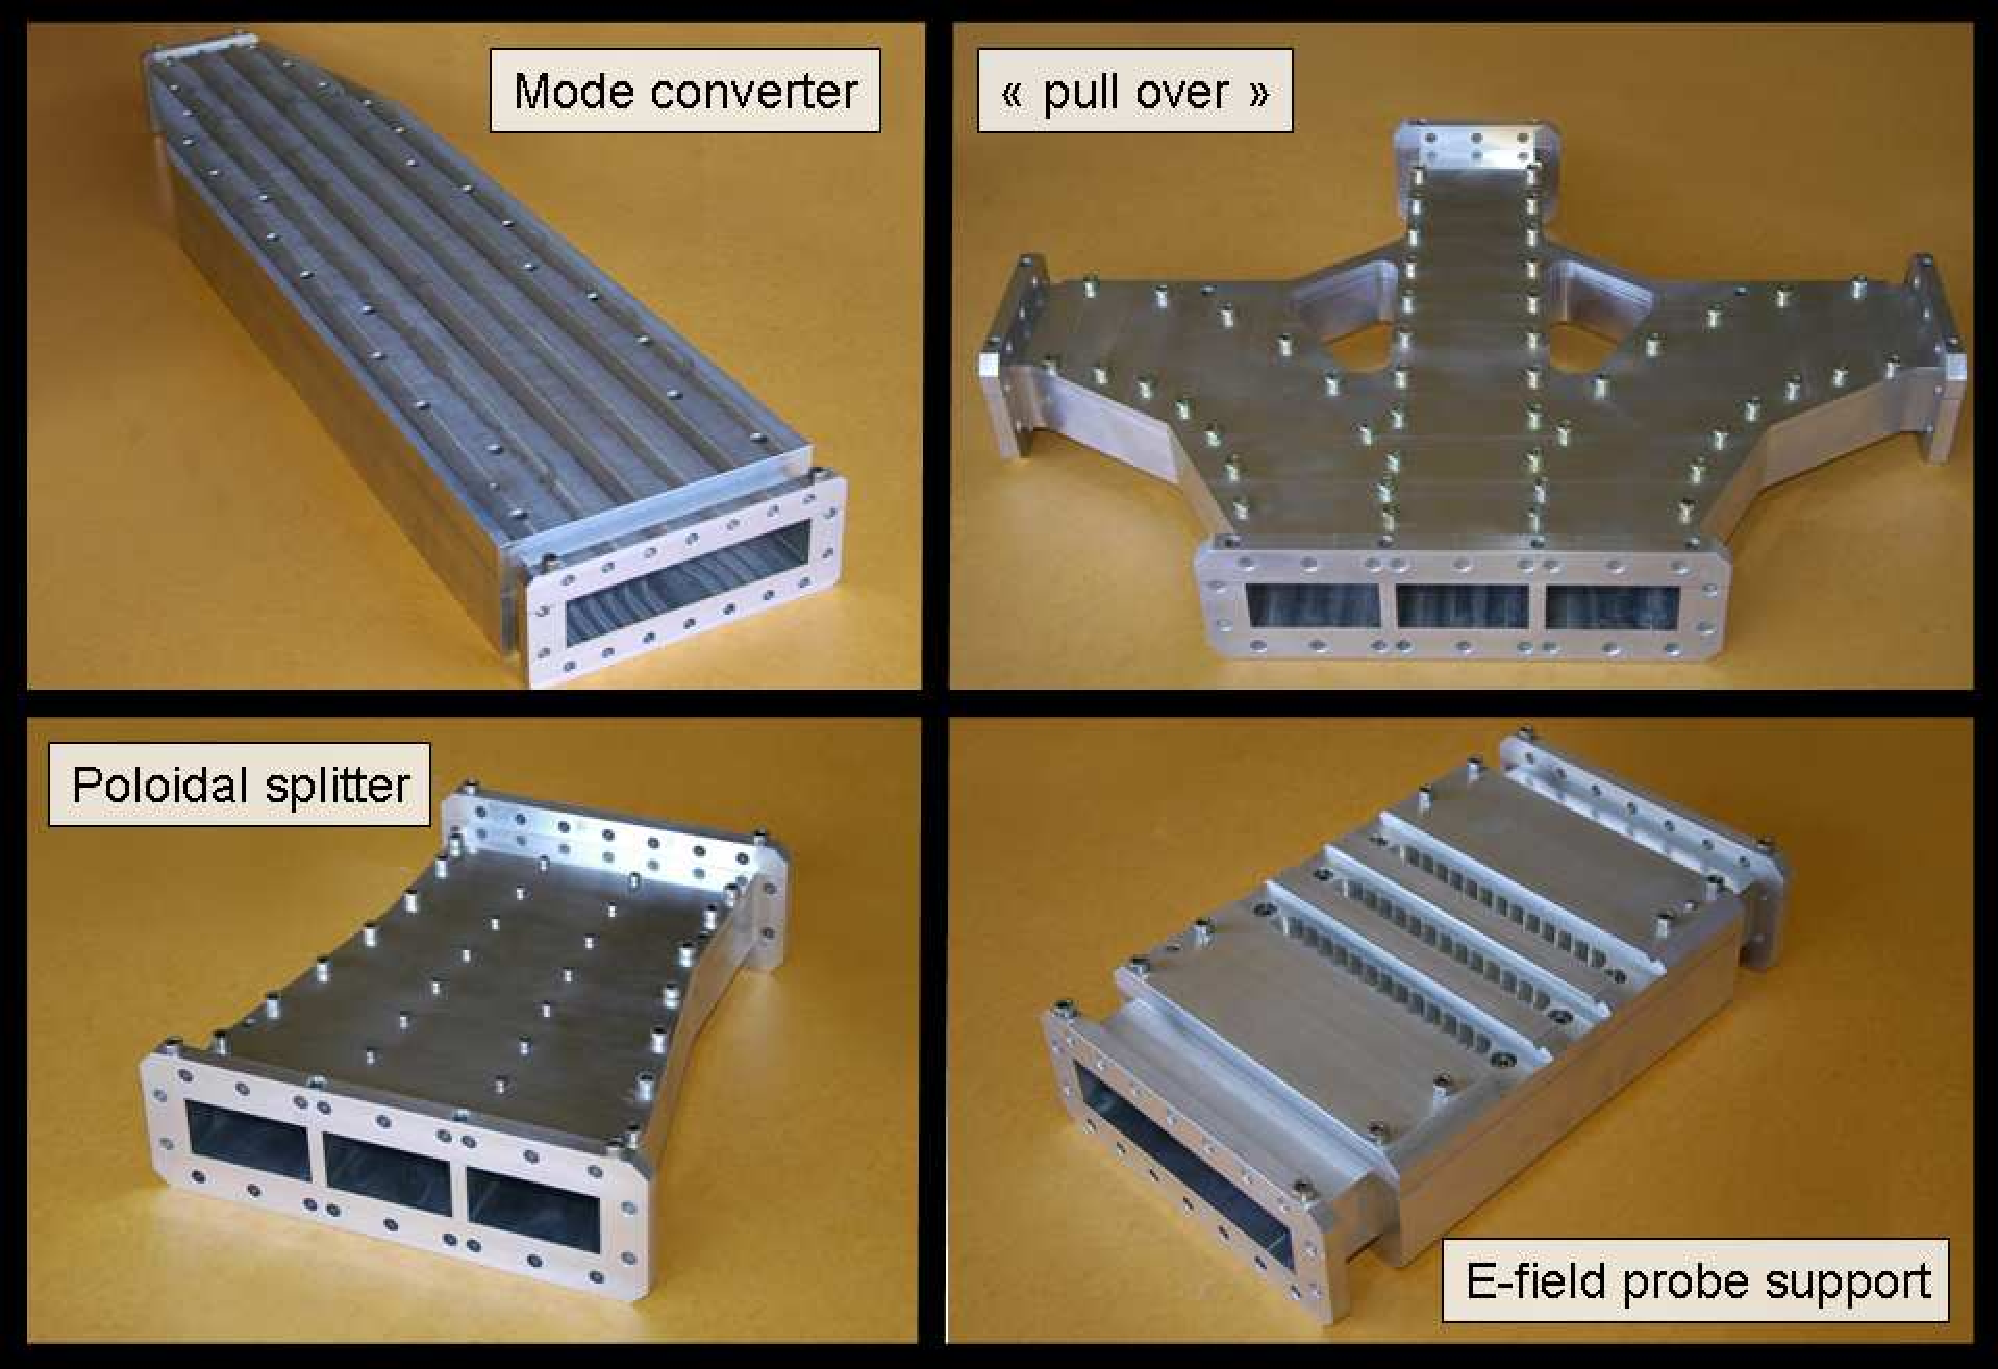
\includegraphics[width=1.0\textwidth]{figures/chap3/ITER_modeconverter/LH4ITER_ModeConverterMockUpElements}
	\caption{Manufactured low RF power mock-up elements. From top left to bottom right: mode converter,  "pull-over" and E-field probe waveguide support. }
	\label{fig:ModeConverterMockUpElements}
\end{figure}

The test bed used to measure the mode converter consisted in the assembly of the mode converter, the poloidal splitter and the ''pull-over''. The aim of this last element is only to facilitate the measurements by putting the output ports aside. Some WR187-WR229 tapers have also been added at each ports in order to match the commercially available WR187 waveguide-to-coaxial transitions (Figure~\ref{fig:RFTestBed}).

\begin{marginfigure}
	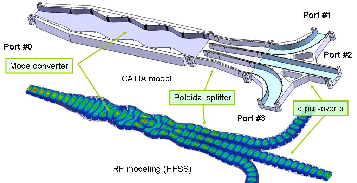
\includegraphics[width=1.0\linewidth]{figures/chap3/ITER_modeconverter/LH4ITER_ModeConverterMockUpCAD}
	\caption{RF Modelling of the complete assembly.}
	\label{fig:lh4itermodeconvertermockupcad}
\end{marginfigure}


\begin{figure}[h]
	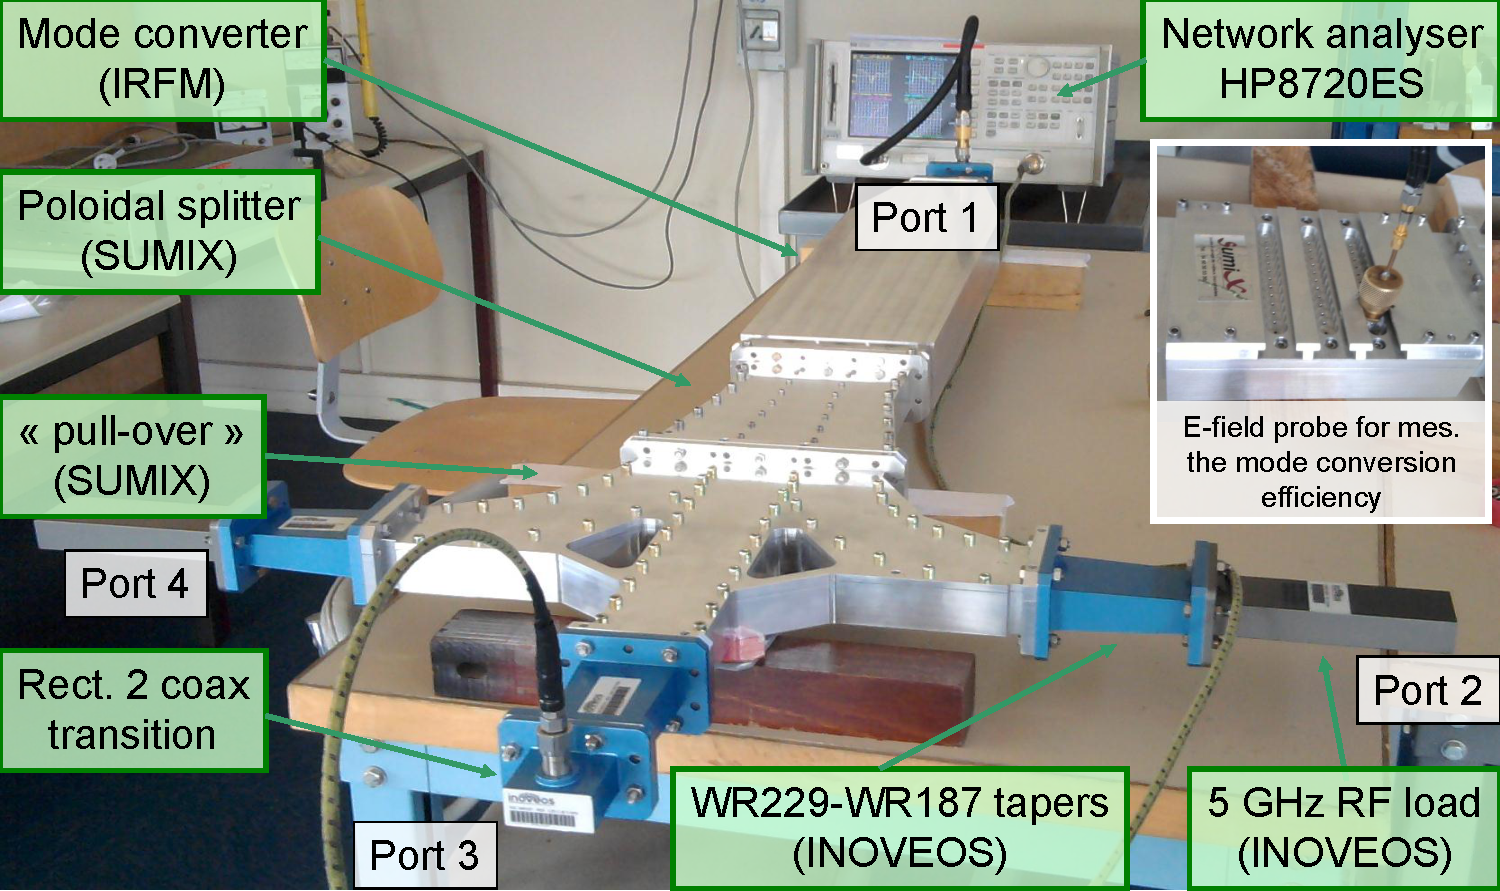
\includegraphics[width=1.0\textwidth]{figures/chap3/ITER_modeconverter/Test_RFTestBed}
	\caption{RF test bed. The pull-over (bent connection waveguides) and the E-field probe support are only used for low-power RF measurements.}
	\label{fig:RFTestBed}
\end{figure}

RF measurements indicate a return loss of 40~dB and a transmission loss of 4.78~dB $\pm$~0.03~dB for the three ports, very close from the ideal 4.77~dB corresponding to the third of the input power. Amplitude measurement results are illustrated in Figures \ref{fig:ModeConverter_S11} and \ref{fig:ModeConverter_S21}; results are in good agreement with the numerical modelling of the complete assembly. The phase shift between the side ports and the center port is $180\deg\pm5\deg$ as expected by the modelling. 

\begin{figure}
	\centering
	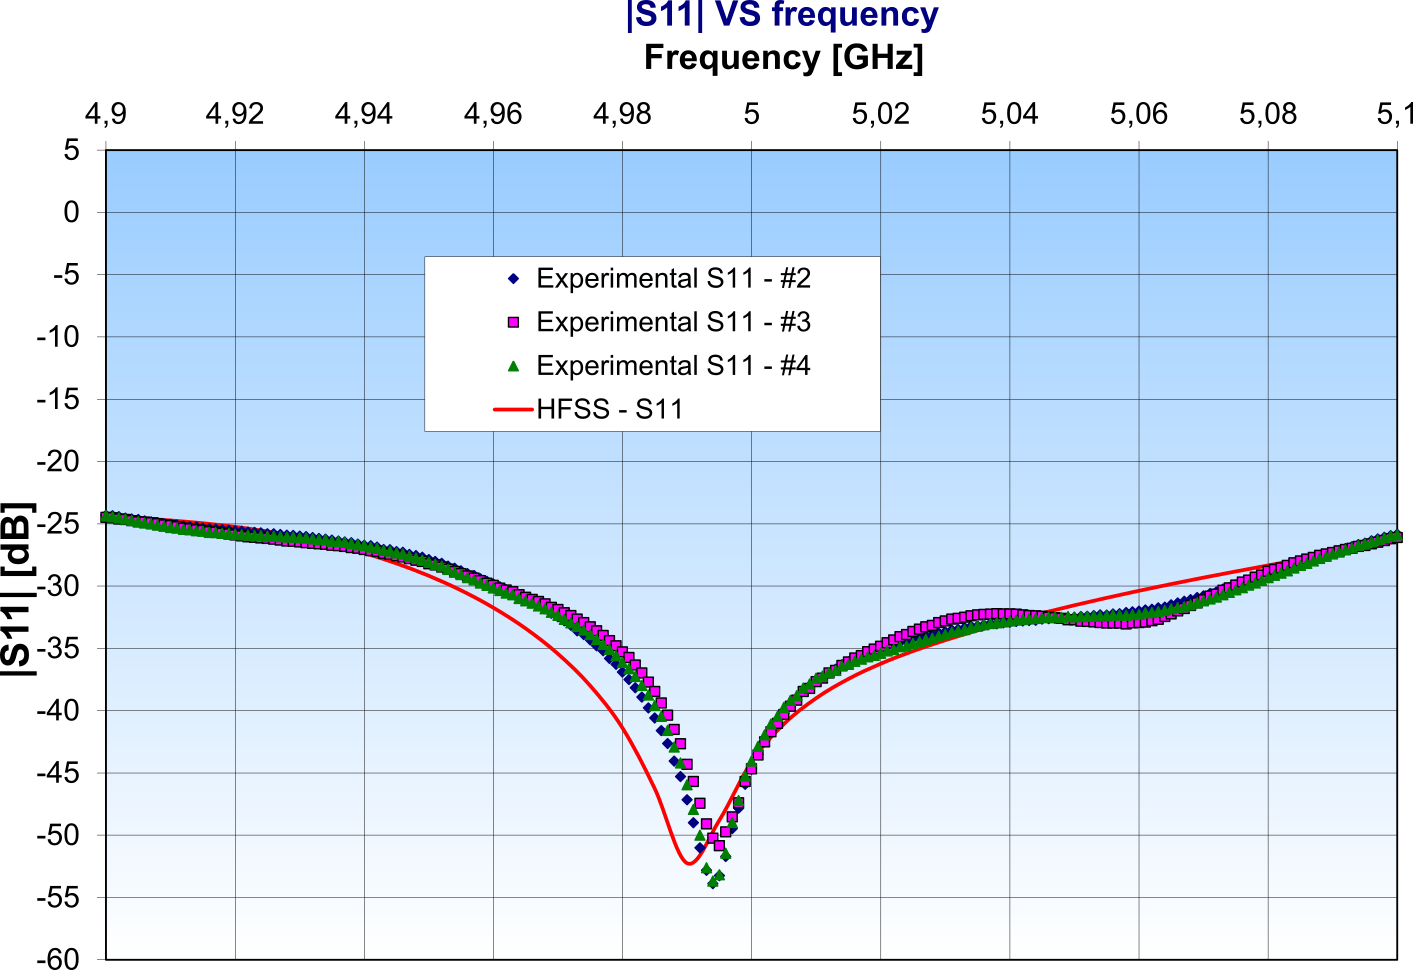
\includegraphics[width=1.0\textwidth]{figures/chap3/ITER_modeconverter/LH4ITER_ModeConverter_S11}
	\caption{Reflexion scattering parameter $|S_{11}|$ of the mode converter over the 4.9-5.1~GHz frequency band. HFSS modeling results are illustrated for comparison. Three measurements have been made, corresponding to the network analyzer second port location on port 2, 3 or 4.}
	\label{fig:ModeConverter_S11}
\end{figure}

\begin{figure}
	\centering
	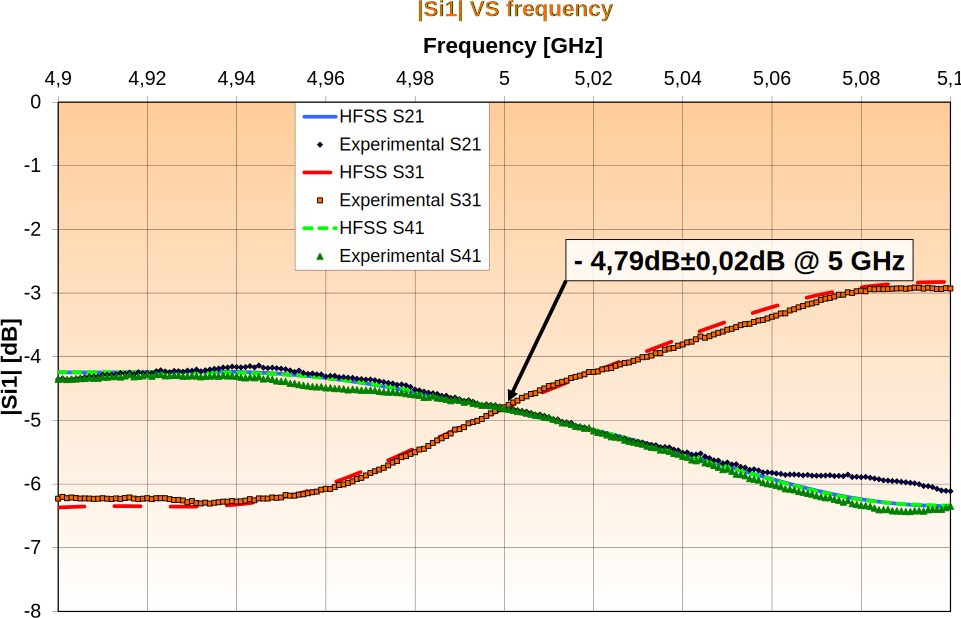
\includegraphics[width=1.0\textwidth]{figures/chap3/ITER_modeconverter/LH4ITER_ModeConverter_S21}
	\caption{Transmission scattering parameters $|S_{i1}|$ of the mode converter over the 4.9-5.1~GHz frequency band ($i \in \{2,3,4\}$). HFSS modeling results are illustrated for comparison.}
	\label{fig:ModeConverter_S21}
\end{figure}

\clearpage
% ##############################################
\subsection{Mode Conversion Efficiency}
In order to measure the forward conversion efficiency from $\TE_{10}$ mode to $\TE_{30}$, a dedicated waveguide element has been manufactured. This element allows direct electric field probing of the mode converter output section, in which an almost pure $\TE_{30}$ mode is expected. This element is illustrated in Figures~\ref{fig:ModeConverterMockUpElements} (bottom right picture ) and \ref{fig:RFTestBed}. It consists in a straight waveguide of section $142.8~\si{mm}\times29.08~\si{mm}\times308~\si{mm}$, which matches the output section of the mode converter. Three rows of holes (2~mm diameter, 10~mm spaced) are drilled in the H-plane. These holes are made to support and block the probe in order to make the measurements at the exactly same spatial locations while holding the probe in a vertical position. The probe is inserted inside each hole sequentially and measures the amplitude and the phase of the electric field inside the waveguide. The coupling element is a thin 1mm diameter copper wire.  The probe ground potential is connected to the waveguide. The coupling has been measured to be -49~dB. Once the probe is inserted into a probe hole, the coupling element supersedes the waveguide wall by less than 1 mm. It is supposed from the small dimensions of the probe that the perturbations due to its use are negligible.  

From these electric field measurements, the modal content after the mode converter can then be deduced with the following method\sidenote{This method is not unique. This modelling is given  as exercise to students during the Master Fusion hands-on in Cadarache. Along the year, many different methods have been found and are summarized in  \href{https://github.com/jhillairet/documents/blob/master/notebooks/TP\%20Master\%20Fusion/LH-Hands-on-multijunction.ipynb}{this Jupyter Notbook}. }. We first assume that the electromagnetic field inside the waveguide is a linear combination of $\TE_{m0}$ modes only, then from at a point $(x,z)$ of the waveguide we have from Eq.(\ref{eq:rectwg_transverse_fields_sum_modes}):
\begin{equation}
\Ebf_{t}(x,z)
	=
	\sum_{m=1}^{N_{modes}}
	A_{m} \ebf_{m}^{+} \left(x,z\right) + B_{m} \ebf_{m}^{-} \left(x,z\right) 
\end{equation}
where $x$ is the largest side direction and $z$ is the propagation direction. The $\ebf_{m}^{\pm}$ terms are the analytic modal eigenfunctions describing forward and backward $\TE_{m0}$ modes shapes given in Eqs.(\ref{eq:TEmodes_eingenfunctions}). $A_{m}$ and $B_{m}$ are the associated forward and backward weight coefficients.  The aim of the method is to find the $2\times N_{modes}$ best coefficients $A_{m}$,$B_{m}$  in order to minimize the squares of the error $\chi^{2}$ between the theoretical field and the measured field:
\begin{equation}
\chi^{2}\left(A_{m},B_{m}\right)=\sum_{i=1}^{N_{mes}}\left(E_{mes,i}-E_{th,i}\right)^{2} 
\end{equation}
Solving this problem leads to the forward $A_{m}$ and backward $B_{m}$ coefficients, and thus to the forward mode conversion efficiency which can be defined as the ratio between the power carried by the $\TE_{30}$ over the power carried by all forward modes, i.e:
\begin{equation}
\eta=\frac{\left|A_{3}\right|^{2}}{\sum_{n}\left|A_{n}\right|^{2}}\times100
\end{equation}

This efficiency has been calculated from the electric field probing after the mode converter to be $\eta=99.9$\%. 



% #####################################################
\subsection{Summary of this Section}
In the frame of the Lower Hybrid R\&D for ITER activities conducted at CEA/IRFM, a low power mock-up of a $\TE_{10}-\TE_{30}$ mode converter at 5~GHz has been designed, manufactured and successfully validated with low power RF measurements. The next section is dedicated to another ITER LHCD system component, the RF windows.  

\clearpage
% #####################################################
% #####################################################
\section[ITER RF Window]{5 GHz ITER RF Window Design and Tests}\label{sec:RF_windows}
% ############################################
\subsection{Context}
\marginnote{Parts of this section are taken from \citeauthyear{hillairet2015}.}
A tokamak operates at pressures different from the transmission line pressure. RF windows intend to isolate these different pressures but allow propagation of the microwaves with low losses and limited RF power reflection. Vacuum vessel operates at ultra-low pressure, typically $10^{-4}$ to $10^{-6}$~\si{Pa}, while transmission lines can contain atmospheric pressure or pressurized gas to increase the breakdown voltage. Consequently, the window must be sufficiently strengthened to withstand differential pressures of the order of several tens of \si{kPa}. On the other hand, window must withstand mechanical stresses such as shock and vibration, and important temperature variations. Window failures can be caused by reflected power, vacuum arcs/multipactor or too much heat dissipation \sidecite{vaughan1961, ikeda1989, neuber1998, hemmert1998}. In the case of a fusion reactor such like ITER, the windows are also part of the first nuclear confinement barrier.

As the dimensions of the tokamak access ports are limited, the number of transmission lines connected to the antenna is limited too. In order to fit into the available space, to simplify the assembly design and to improve the maintenance of the system, the number of transmission lines and thus the number of RF windows must be kept as low as possible. This leads to increase the power handling capability of each transmission line, and ultimately of each window.

In the proposed ITER LHCD design (Cf. Section~\ref{sec:ITER_LHCD_antenna}), 24~\si{MW}~CW of RF power at 5~\si{GHz} are expected to be generated and transmitted to the plasma. In order to separate the vacuum vessel pressure from the cryostat waveguide pressure, forty eight 5~\si{GHz} 500~\si{kW} windows are to be assembled on the waveguides at the equatorial port flange. For nuclear safety reasons, 48 additional windows could be located in the cryostat section, to separate the cryostat waveguide pressure from the exterior transmission line pressure and to monitor it. Because the failure of a window would lead to lock a transmission line, these windows have been identified as one of the main critical components for the ITER LHCD system since first ITER LHCD studies \sidecite{bibet2005}. In order to initiate this R\&D effort, two 5~\si{GHz} 500~\si{kW}/5~s pill-box prototype windows have been developed and manufactured in 2012 by the PMB/ALCEN Company in close collaboration with the CEA/IRFM\sidecite{hillairet2014, hillairet2015}. 

% ############################################
\subsection{RF and Thermo-Mechanical Design}
% TODO: \usepackage{graphicx} required
\begin{marginfigure}
	\centering
	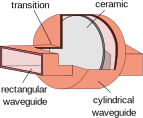
\includegraphics[width=1.0\linewidth]{figures/chap3/pillbox_window}
	\caption{Pill-box window schematics}
	\label{fig:pillboxwindow}
\end{marginfigure}

The proposed ITER 5~\si{GHz} RF window is based on a pill-box window concept \sidecite[+4cm]{ives1993,maebara1995}, i.e. a thin ceramic disc brazed in the middle of a short straight section of a circular waveguide axially connected on both sides to rectangular waveguides as illustrated in Figure~\ref{fig:pillboxwindow}. According to the transmission line theory, the pill-box window has four discontinuities: rectangular waveguide to circular waveguide, vacuum to ceramic and ceramic to vacuum and circular waveguide to rectangular waveguide. Typical design rule of thumb of such device is circular section diameter about the same size of the diagonal of the rectangular waveguide. Without taking into account the ceramic, the circular section length is approximately half a guided wavelength of the circular $\TE_{11}$ mode, in order to not generate spurious reflection into the rectangular sections. For a prescribed dielectric properties, the RF design consists in optimizing the geometrical dimensions of the window, mainly the diameter, the ceramic thickness and the vacuum circular waveguide length in order to minimize both RF reflection (matching) and RF power absorption in the ceramic (from trapped or ghost-mode heating \cite{ives1993} ). Once optimized, taking into account the ceramic, the matching is optimum only for a narrow band of frequency and is very sensitive to the device dimensions and the ceramic relative permittivity. As the klystrons used for fusion applications have narrow bandwidth, for instance 5~MHz at 3.7~GHz \sidecite[-1cm]{beunas2009, magne2011} or 5~GHz klystrons \sidecite{kenichihayashi2007, park2013}, the RF optimization is performed for the central frequency only. 

The heat losses in the ceramic, which have to be extracted by an active water cooling, depend on both the inside electric field topology and the ceramic dielectric loss (loss tangent). Undesirable modes due to parasitic resonances can be excited in the ceramic volume, raising the electric field and thus the heat dissipation. This aspect is uncorrelated from the return loss and one can even achieve low return loss but can have high heat losses in the ceramic (>2~\si{kW}) \sidecite{mirizzi2011}. So both aspects have to be taken into account during the RF optimization process.


\begin{marginfigure}
	\centering
	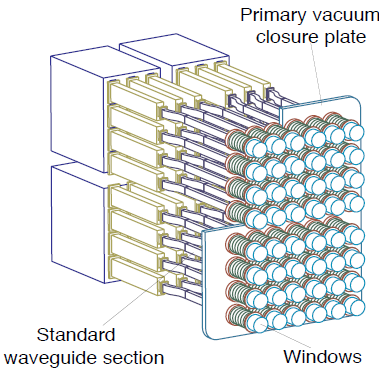
\includegraphics[width=1.0\linewidth]{figures/chap3/ITER_antenna/ITER_LH_antenna_old}
	\caption{ITER 2001 Conceptual Design from \cite{bibet2001-1}}
	\label{fig:iterlhantennaold}
\end{marginfigure}


In the 2001 initial Lower Hybrid (LH) antenna design, 24 RF windows were set on the cryostat port. Each of them fed 2 RF windows installed on the vacuum port (illustrated in Figure~\ref{fig:iterlhantennaold}). Since the antenna is designed for a power up to 20 MW, each RF window of the first and second group have to withstand respectively 833 kW CW and 417 kW CW. Two preliminary designs had been proposed in \sidecite[+3.5cm]{bibet2001-1}. However, the mechanical analysis performed in \sidecite[+4cm]{hoang2009-2} showed that stresses are higher than the static fatigue limit of 50 MPa. This particularly point invalidates the design for dynamic fatigue (cycles of repeated heating and cooling). Following this study, a new RF design has been developed. At the contrary of the model proposed in \cite{bibet2001-1}, a larger rectangular input section has been used (WR229 instead of WR187). It was found in \sidecite[+2cm]{hillairet2013} a range of dielectric thickness which combines low total dielectric losses (<650W) by minimizing the axial electric field in the ceramic and a low VSWR (S11<-25dB). We did not take into account in this study the impact of non-negligible amount of reflected power (>5\%), such as experimented on tokamak.

As highlighted in \sidecite{ao2014}, the relative dielectric properties of the ceramic disk depend on the manufacturer, even when the same manufacturer and ceramic batch are used. At the frequency of 5~GHz, the dielectric losses (loss tangent) of aluminium oxide (Al2O3), aluminium nitride (AlN) or Beryllium Oxyde (BeO) are of the same order ($\tan\delta \approx 10^{-4}$). The choice for BeO ceramic is motivated by its larger thermal conductivity (in the range of 330 to 370~\si{W/m/K} at room temperature) than the other ones (in the range of 30~\si{W/m/K} for Al2O3 and 70-180~\si{W/m/K} for AlN). BeO is used in high power 3.7~GHz and 5~GHz klystrons windows. In order to determine the final thickness of the windows, the BeO ceramic RF properties must be known with accuracy. A BeO sample has been requested from the ceramic manufacturer (American Beryllia) with the guarantee that the final ceramics will be made from the same lot. The sample has been characterized within a RF resonant cavity setup in collaboration with the XLIM laboratory\footnote{The authors thanks Olivier Tantot and Damien Passerieux from the XLIM Laboratory in Limoges, France, where the dielectric measurements on BeO samples have been conducted.} \sidecite[+6cm]{lefloch2014}. The measurement of the BeO sample has been made at two surrounding frequencies and the results are given in \citeauthyear{hillairet2015}. The relative permittivity and the loss tangent at 5~GHz have been calculated from a linear interpolation of the measured values, to be $\varepsilon_{r}=6.36\pm0.159$ and $\tan \delta = 4.30\times 10^{-4}\pm3.82\times 10^{-5}$ respectively. 

\begin{marginfigure}[-3cm]
	\centering
	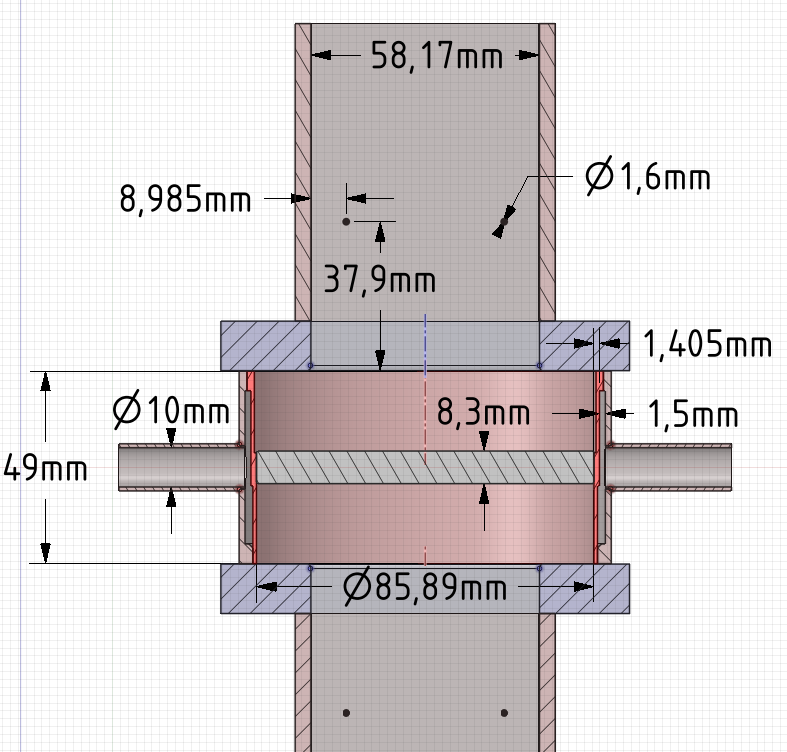
\includegraphics[width=1.0\linewidth]{figures/chap3/ITER_window/ITER_windows_main_dimensions}
	\caption{Main dimensions of the final 5 GHz RF window prototype. }
	\label{fig:iterwindowsmaindimensions}
\end{marginfigure}

From these measurements, the final dimensions have been calculated by the PMB/ALCEN Company in collaboration with CEA. In the proposed design, a rectangular waveguide of section 58.17x29.08~\si{mm} (WR229 standard) is used to forward the RF power into the circular section. The ceramic disk diameter and the thickness are 85.89~mm and 8.3~mm respectively. Other dimensions are reported in Figure~\ref{fig:iterwindowsmaindimensions}. In order to increase the RF performance of the window, in particular the return loss, two matching inductive rods have been added on each side of the window. These rods also make possible an eventual post-manufacturing tuning, by slightly deforming them after the final assembly. This technique has also been used in the TED 3.7~GHz windows used on the Tore Supra tokamak, but with a larger rod diameter due to the reduced frequency. 

\begin{marginfigure}
	\centering
	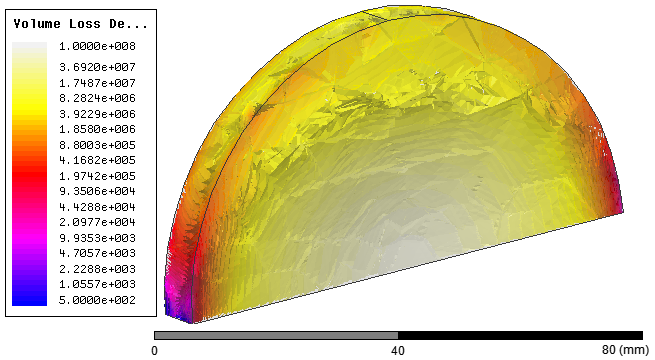
\includegraphics[width=1.0\linewidth]{figures/chap3/ITER_window/ITER_windows_RFlosses_ceramic}
	\caption{Dielectric Losses in the ceramic for 500 kW}
	\label{fig:iterwindowsrflossesceramic}
\end{marginfigure}

The power loss in the ceramic volume and the electric field topology have been evaluated with finite element modelling (Figure~\ref{fig:iterwindowsrflossesceramic}). With the material properties cited above, the calculated dissipated power in ceramic is around 550~W for 500~kW input on matched load. Taking into account a conservative copper conductivity of 4.4~MS/m, the total resistive losses are estimated to 720~W (Figure~\ref{fig:iterwindowsrflosses}). Combined, the expected total RF losses for the window to evacuate is thus of the order of 1.27~kW. 

\begin{figure}
	\centering
	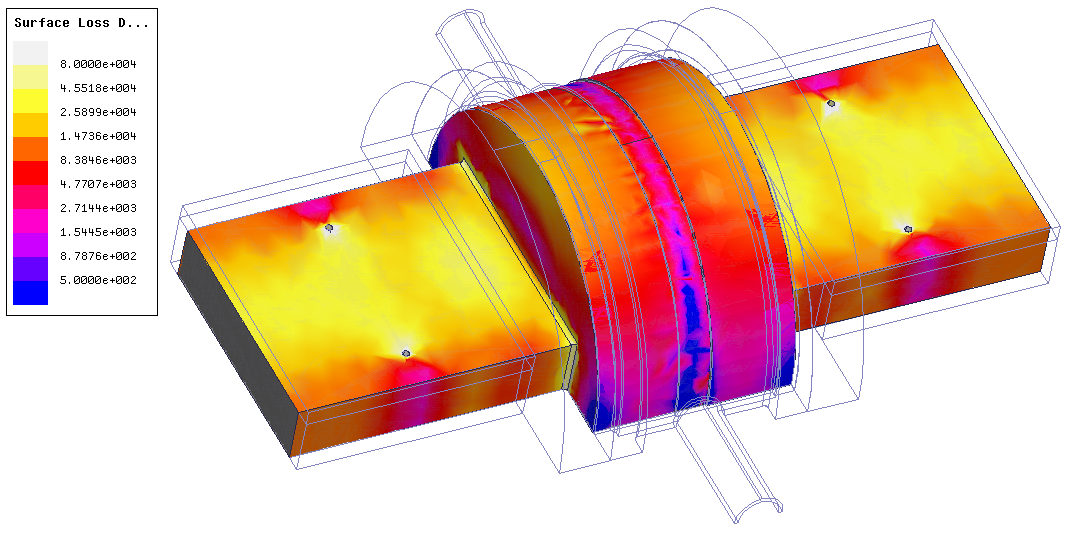
\includegraphics[width=1.0\linewidth]{figures/chap3/ITER_window/ITER_windows_RFlosses}
	\caption{RF Losses on metallic parts of the window.}
	\label{fig:iterwindowsrflosses}
\end{figure}


In order to conform to ITER acceptance criteria for vacuum feedthroughs \sidecite{waldon2008}, the maximum pressure on the ceramic (air) has been specified to be 3~bars absolute (0.3~MPa). The water cooling circuit specifications has been specified in accordance with the NFRI 5~GHz klystron test-bed in which the high power tests have been performed\sidecite{do2011, kim2019-2}. The maximum pressure on the cooling circuit has been set to 6~bars, with a maximum pressure drop on the cooling circuit for a 8~L/min flow of 0.3~bar\footnote{It has to be noted that these specifications are well below the ITER port plug specifications, for which the water temperature and pressure are expected to be 70-100$\si{\celsius}$ up to 40~bars in cooling mode and up to 250$\si{\celsius}$ and 45~bars in baking mode. However, such conditions are challenging because the copper skirt thickness has to be increased to sustain such a pressure. Increasing the skirt thickness in order to withstand a 40-45~bars pressure will reduce the cooling efficiency. Moreover, if the skirt is thicker, the mechanical constraints on the ceramic due to the differential thermal expansion between the BeO and Cu will be more severe since the skirt will be stiffer. For this reason, the present proposed prototype design only focuses on the RF performances.}. 

Assuming an inlet flow of 8~L/min and an outlet return pressure of 1.5~bar specified by the water cooling loop system, the fluid velocity calculated from computational fluid dynamics (CFD) modelling in ANSYS Fluent at the 10~mm diameter inlet is 1.7~m/s. Figure~\ref{fig:iterwindowswatervelocity} illustrates the water velocity in half of the cooling section. The flow in the fluid section is mainly turbulent, as the Reynold number at the inlet/outlet is of the order of 10000 and 40000 in the skirt. Since inlet and outlet have been located normal to the skirt, the water velocity rise up to 4.6 m/s at the interface between the pipe and the skirt. However, the flow is rapidly homogenous in the skirt and with lower velocities (cf. Figure~\ref{fig:iterwindowswatervelocity_closeup_skirt}), leading to an homogenous cooling of the ceramic. The average value of the heat transfer coefficient is H=12300~\si{W.m^{-2}K^{-1}} on the inner side of the skirt. The water pressure is homogenous inside the skirt and the estimated pressure drop is 0.12~bar. Cavitation regime is not expected in the cooling section, as the cavitation number is more than two orders of magnitude above the critical threshold ($\mathrm{Ca}\approx 1$) in all situations.\marginnote{The \href{https://en.wikipedia.org/wiki/Euler_number_(physics)}{Cavitation number} ($\mathrm{Ca}$) is a dimensionless number used in flow calculations. It expresses the relationship between the difference of a local absolute pressure from the vapor pressure and the kinetic energy per volume, and is used to characterize the potential of the flow to cavitate. }

\begin{figure}
	\centering
	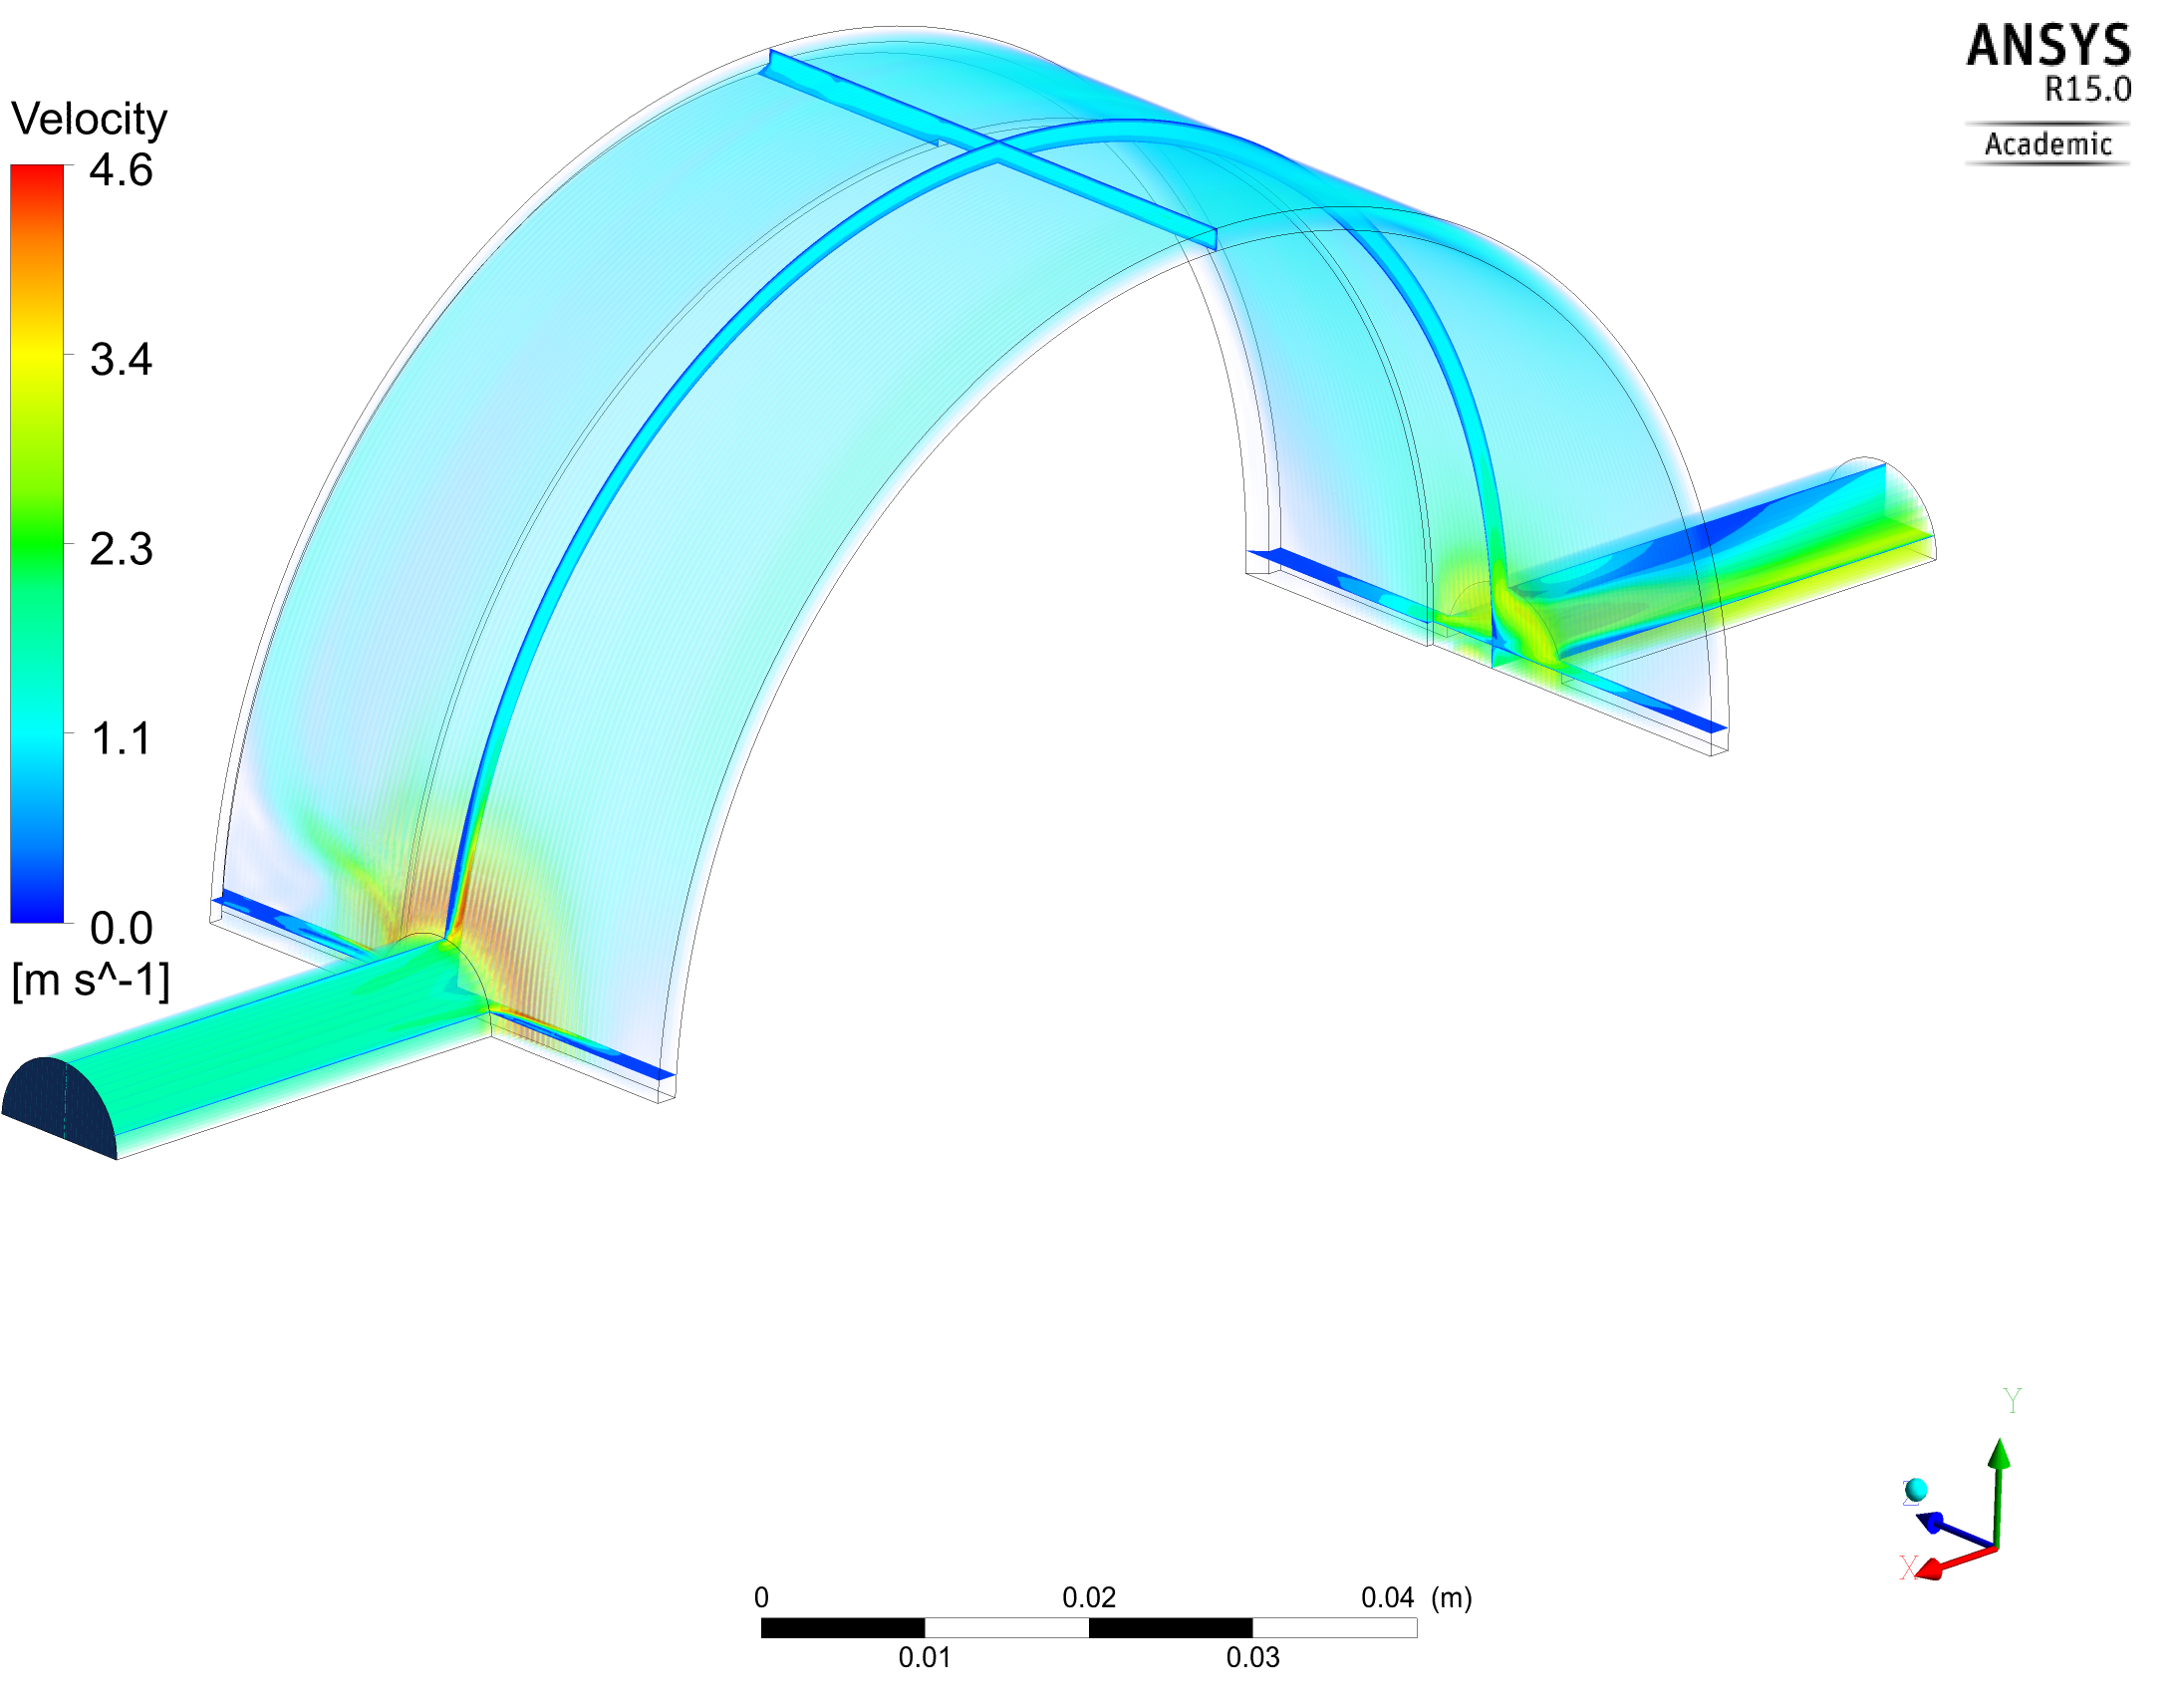
\includegraphics[width=1.0\linewidth]{figures/chap3/ITER_window/ITER_windows_water_velocity}
	\caption{Water velocity in the skirt around the ceramic. Inlet is located at the left of the picture. The black oval illustrates the close-up view of Figure~\ref{fig:iterwindowswatervelocity_closeup_skirt}.}
	\label{fig:iterwindowswatervelocity}
\end{figure}

\begin{marginfigure}[-5cm]
	\centering
	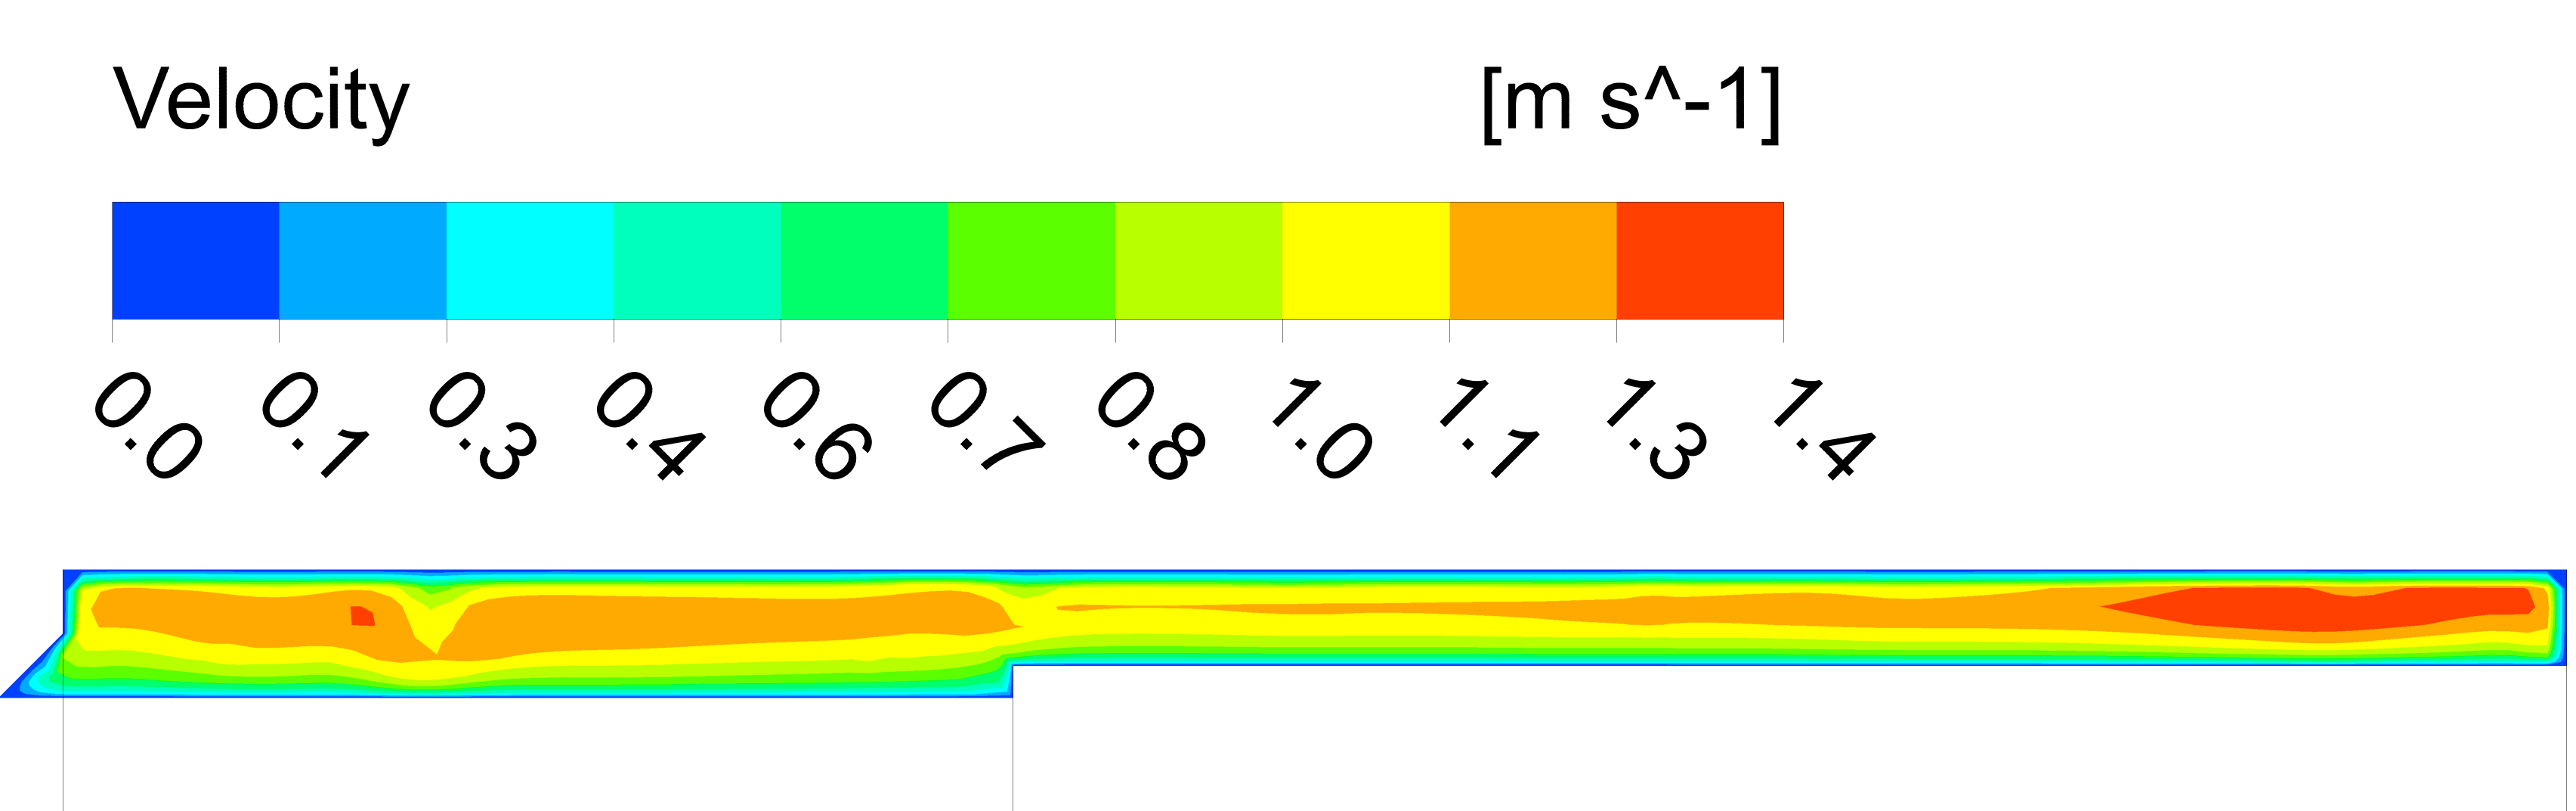
\includegraphics[width=1.0\linewidth]{figures/chap3/ITER_window/ITER_windows_water_velocity_closeup_skirt}
	\caption{Close-up of the fluid velocity in the skirt section.}
	\label{fig:iterwindowswatervelocity_closeup_skirt}
\end{marginfigure}

The thermal model of the window has been set-up using loading from both the electromagnetic (heat load on walls and ceramic) and CFD models (convection on the skirt). A first thermal steady-state study has been conducted to survey the maximum reached temperature. The thermal loads come from the RF losses in the ceramic and on the waveguides walls and coupled to the thermal model. The thermal sinks come from water cooling and air radiation. The rectangular waveguide parts and the skirt are modelled as OFHC copper. The connections between the elements, especially between the BeO and the copper skirt, are modelled as perfect (bonded). The mechanical parameters of the BeO used in the thermal model are reported in \cite{hillairet2015}. The thermal conductivity of the BeO has been kept constant with respect to the temperature. However some studies indicate however that the thermal conductivity drops with temperature\sidecite{defaoite2012}, which would increase the BeO temperature. 

As the matching rods are not directly cooled by the water circuit, their temperatures reach 180$\si{\degreeCelsius}$ after a 5 seconds pulse and nearly 290$\si{\degreeCelsius}$ in steady-state regime. For this reason, the nominal RF pulse duration of these prototypes has been limited to be 5 seconds as a conservative approach. For a CW design, cooling pipes on the upper and lower parts of the rectangular waveguides would solve the problem.

In the ceramic, the maximum temperature is reached at the centre where the dielectric loss density is the maximum and which is also the farthest point from the water heat sink. Starting from an initial water temperature of 22$\si{\degreeCelsius}$, the ceramic centre temperature is calculated to be 75$\si{\degreeCelsius}$ after a 5 s/500 kW pulse (Figure~\ref{fig:iterwindows_thermal_modeling}). The initial temperature of the ceramic is recovered after nearly 10 s, as illustrated in Figure 8. In order to limit the mechanical stresses on the ceramic, the temperature difference between the centre and the periphery of the disk must be kept under a safety limit of 80$\si{\degreeCelsius}$. This limit has been determined by both mechanical modelling and rule of thumb, in order to keep stresses in the ceramic below the static fatigue limit.

\begin{figure}
	\centering
	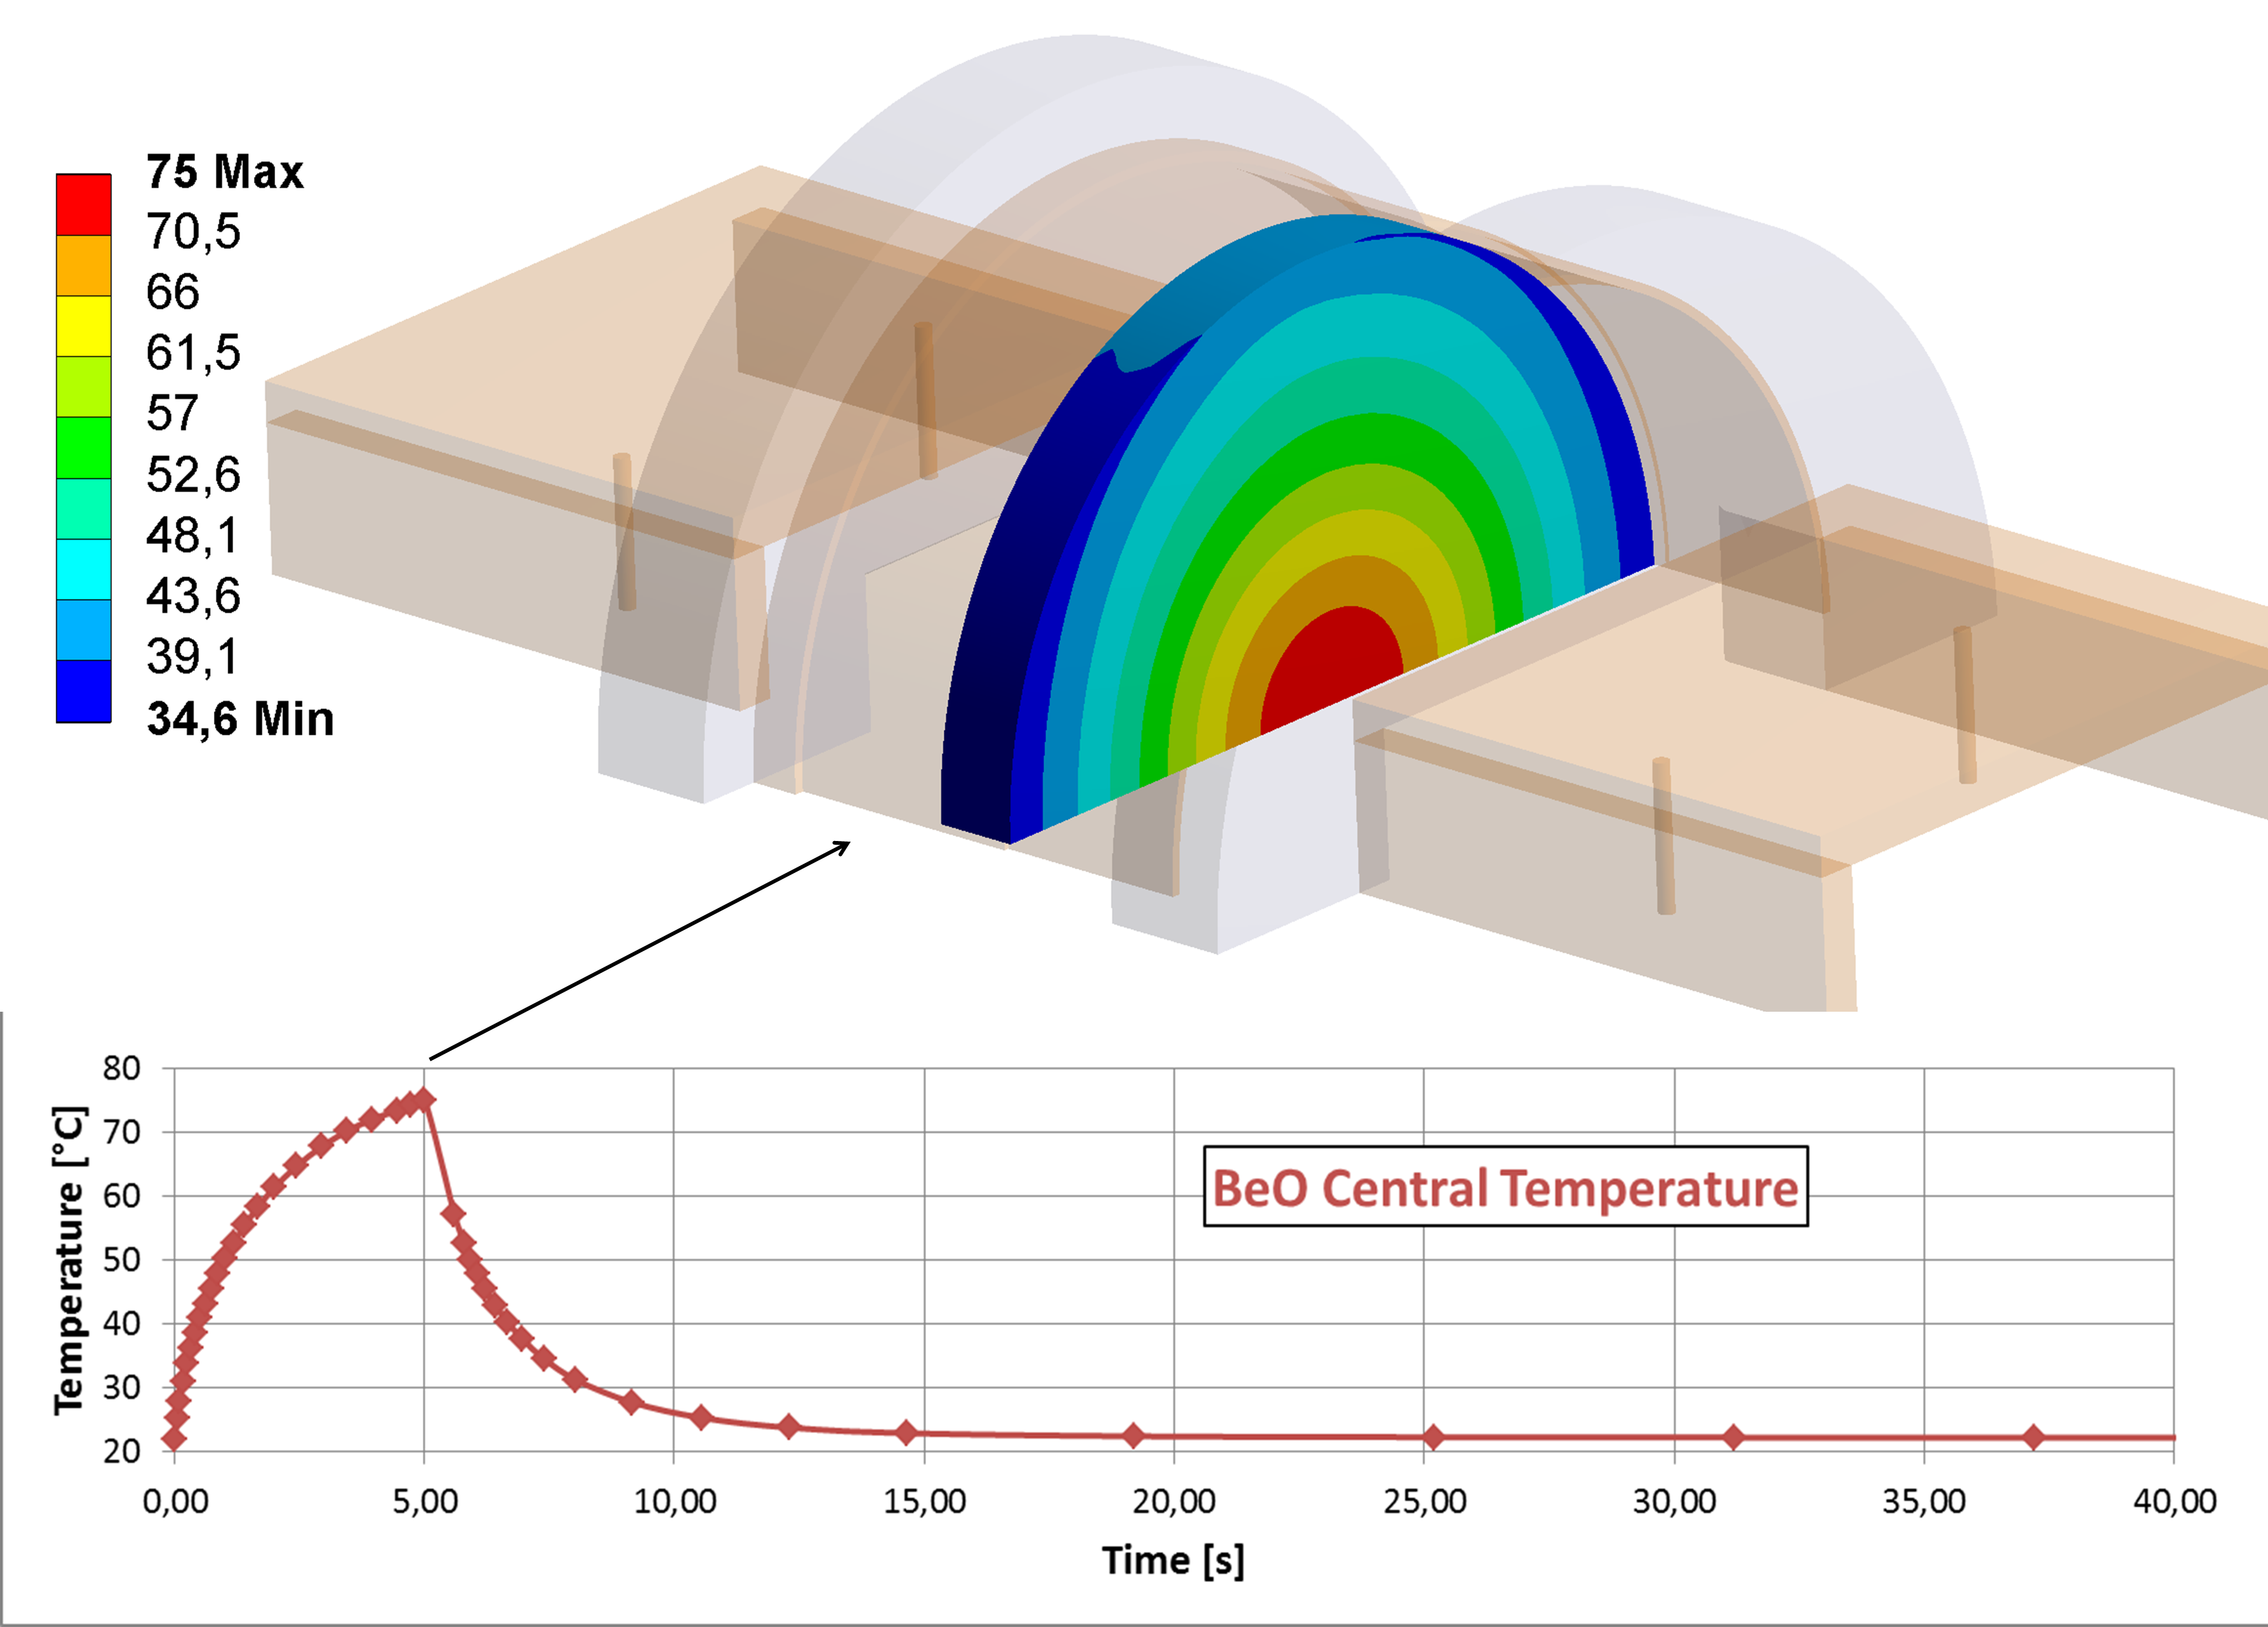
\includegraphics[width=1.0\linewidth]{figures/chap3/ITER_window/ITER_windows_thermal_modeling}
	\caption{Modelling of the temperature evolution of the BeO ceramic during a 5s/500kW RF pulse.}
	\label{fig:iterwindows_thermal_modeling}
\end{figure}

\subsection{Manufacturing and Low Power Tests}\label{sec:ITER_windows_manuf_low_power_tests}
\begin{marginfigure}
	\centering
	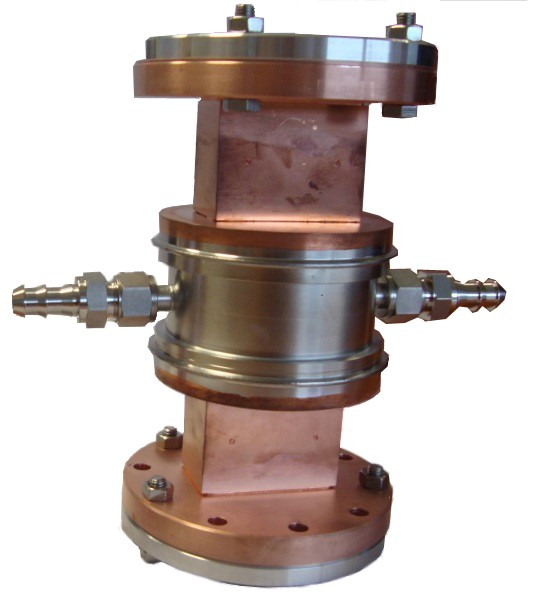
\includegraphics[width=1.0\linewidth]{figures/chap3/ITER_window/ITER_windows_picture}
	\caption{picture of one window}
	\label{fig:iterwindowspicture}
\end{marginfigure}
Two RF windows have been manufactured by the PMB/ALCEN Company in collaboration with CEA/IRFM (Figure~\ref{fig:iterwindowspicture}). For ensuring the possibility to perform ITER relevant tests, like high temperature baking up to 240$\si{\degreeCelsius}$ , the window flanges are non-standard and have been designed to be compatible for both Viton or Helicoflex seals. As shown in Figure~\ref{fig:iterwindowsgeometry}, a rectangular groove is machined on both sides of the window. Male waveguide adapters are then required to connect the window: these adapters are designed to insure a good electrical contact at the flange by a heel slightly longer than the groove depth, in order to dissociate the electrical contact from the sealing aspects. In return, additional elements must be connected together, which can lead to additional losses in the transmission line.   

\begin{figure}
	\centering
	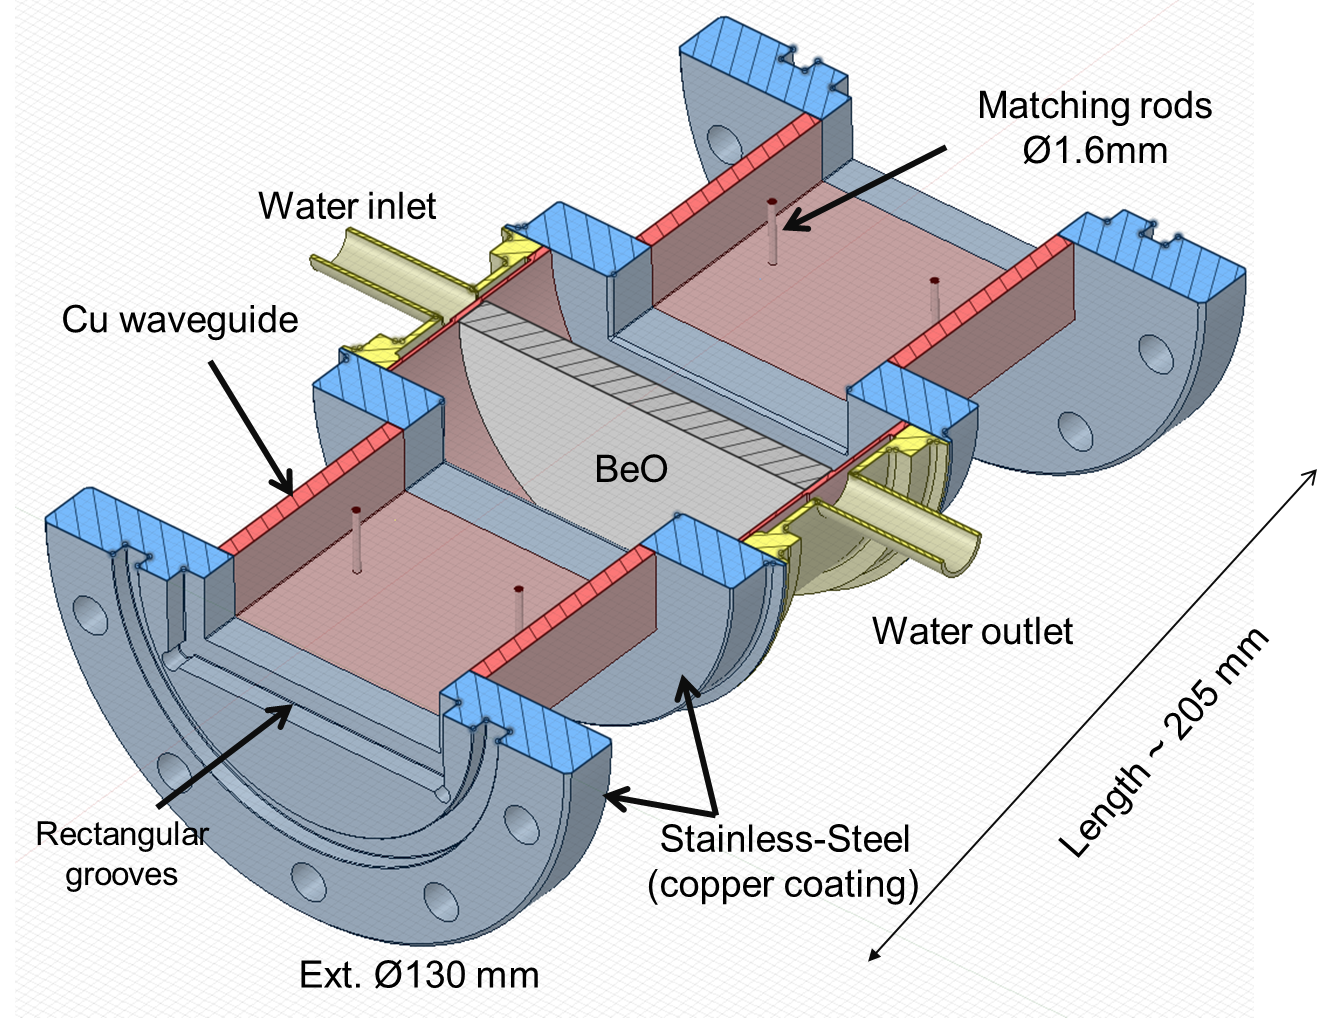
\includegraphics[width=1.0\linewidth]{figures/chap3/ITER_window/ITER_windows_geometry}
	\caption{CAD cut-view of the window.}
	\label{fig:iterwindowsgeometry}
\end{figure}

BeO ceramic has a high secondary electron emission coefficient, which enhances multipactor induced breakdown probability. In order to suppress the multipactor induced breakdown at the surface of the ceramic, a 10~\si{nm} titanium nitride (TiN) coating is applied by vapour deposition. This coating intends to decrease the secondary emission yield of the ceramic and to improve the electrical charge exchange \sidecite{lorkiewicz2004} . Stainless-steel parts facing the RF fields are copper coated (10 to 20~$\si{\mu m}$).  After brazing the rectangular copper waveguides elements together, the stainless-steel parts are TiG welded. 

Low power RF measurements (dBm level) are reported in Figure~\ref{fig:iterwindowsrl} for both windows, labelled \#1 and \#2. The return losses ($S_{11}$ and $S_{22}$) at 5~GHz are below -32~dB (SWR < 1.05:1) in accordance with the RF modelling. The optimum frequency is shifted to low frequencies by 20 to 40~MHz, for reasons that will be explained in the next section. It has to be noted that the return losses $S_{11}$ and $S_{22}$ are not symmetrical for both windows, differently from the results of the RF modelling. This fact is attributed to both the measurement errors (which come from RF cables) and the matching rods which were deformed during manufacturing. These deformations, due to a handling problem during the copper coating operation, have been experienced for both windows. Even if the rods have been reshaped with specific tooling as best as possible, slight mechanical differences exist between each rods (at the contrary of the RF model which is ideal and perfectly symmetric). 

\begin{figure}
	\centering
	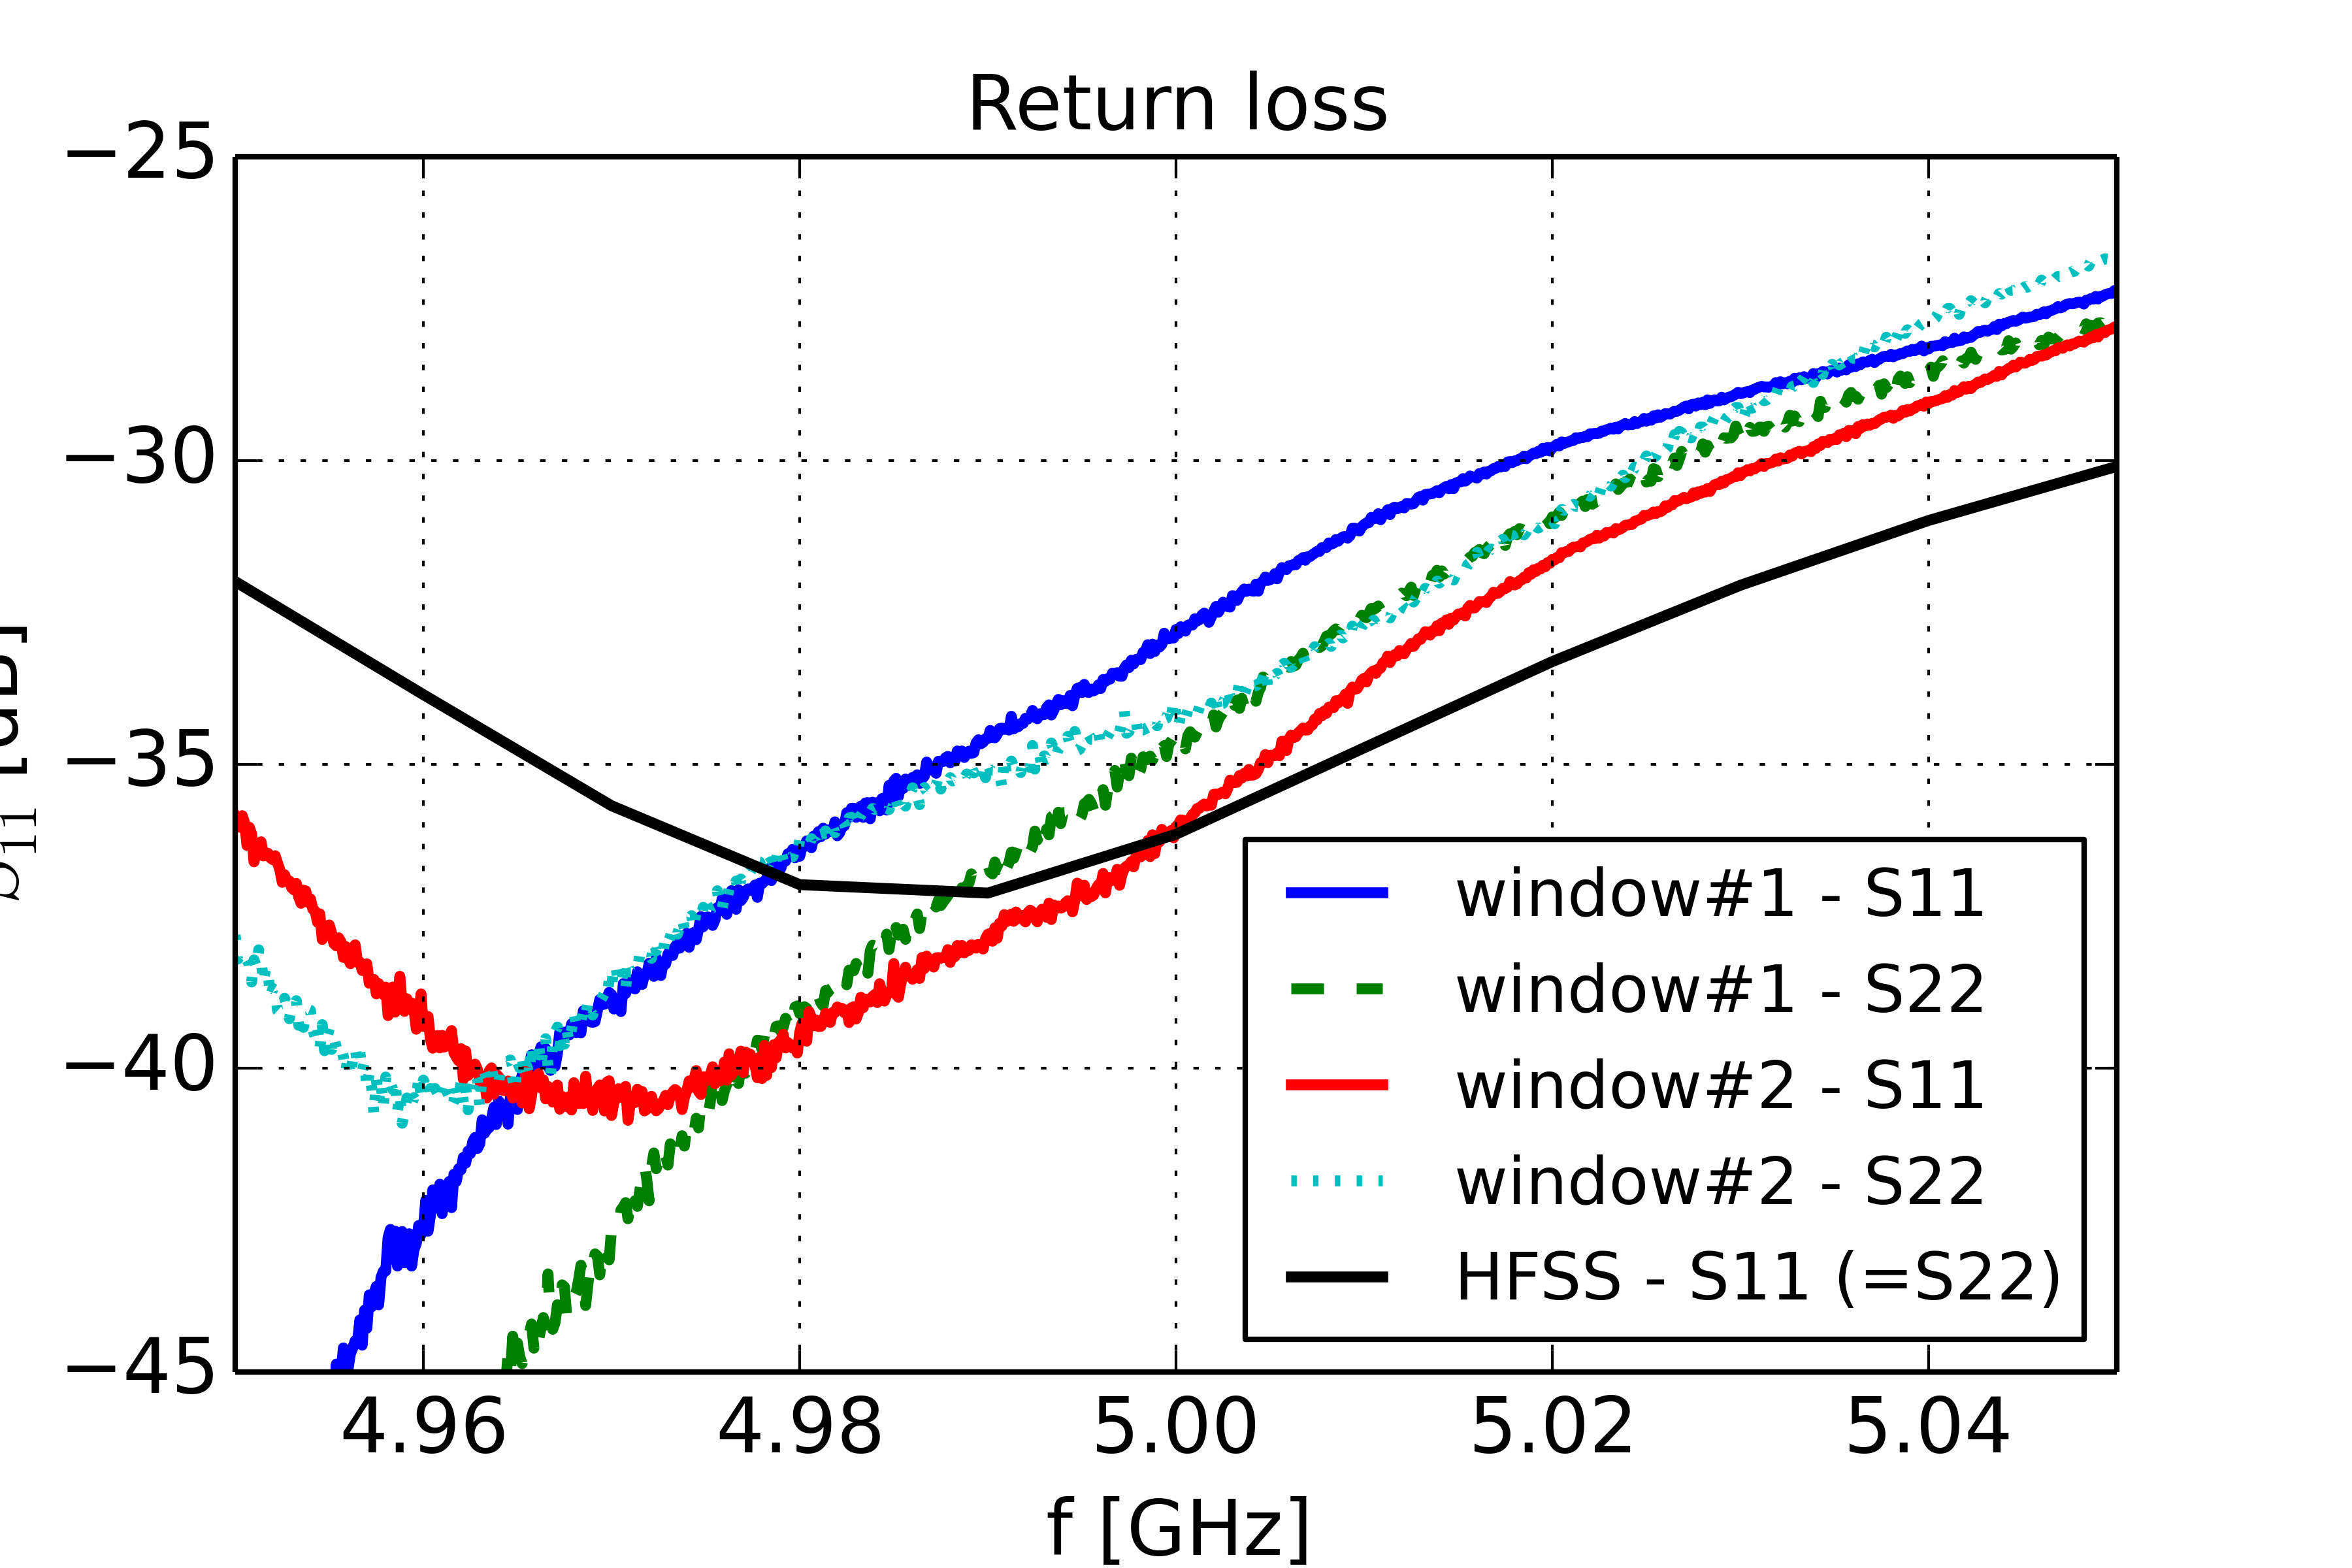
\includegraphics[width=1.0\linewidth]{figures/chap3/ITER_window/ITER_windows_RL}
	\caption{Return loss [\si{dB}] for both windows. RF modelling prediction(plain black) from HFSS}
	\label{fig:iterwindowsrl}
\end{figure}

The insertion losses ($S_{21}$) are reported in Figure~\ref{fig:iterwindowsil}. They have been measured at 5~GHz in the range from -0.01 dB to -0.05 dB (i.e. between 0.23\% and 1.14\% of input power). The overall uncertainty of the transmission losses measurements is of the order of 0.03 dB. These measurements reflected not only the window transmission losses but also the part of the assembly for which no calibration was possible (such as the dedicated waveguides adapters with specific flanges). Precise measurements of the insertion losses are very sensitive to the test bed mechanical assembly, in particular to the quality of the mechanical assembly of all flanges.  

\begin{figure}
	\centering
	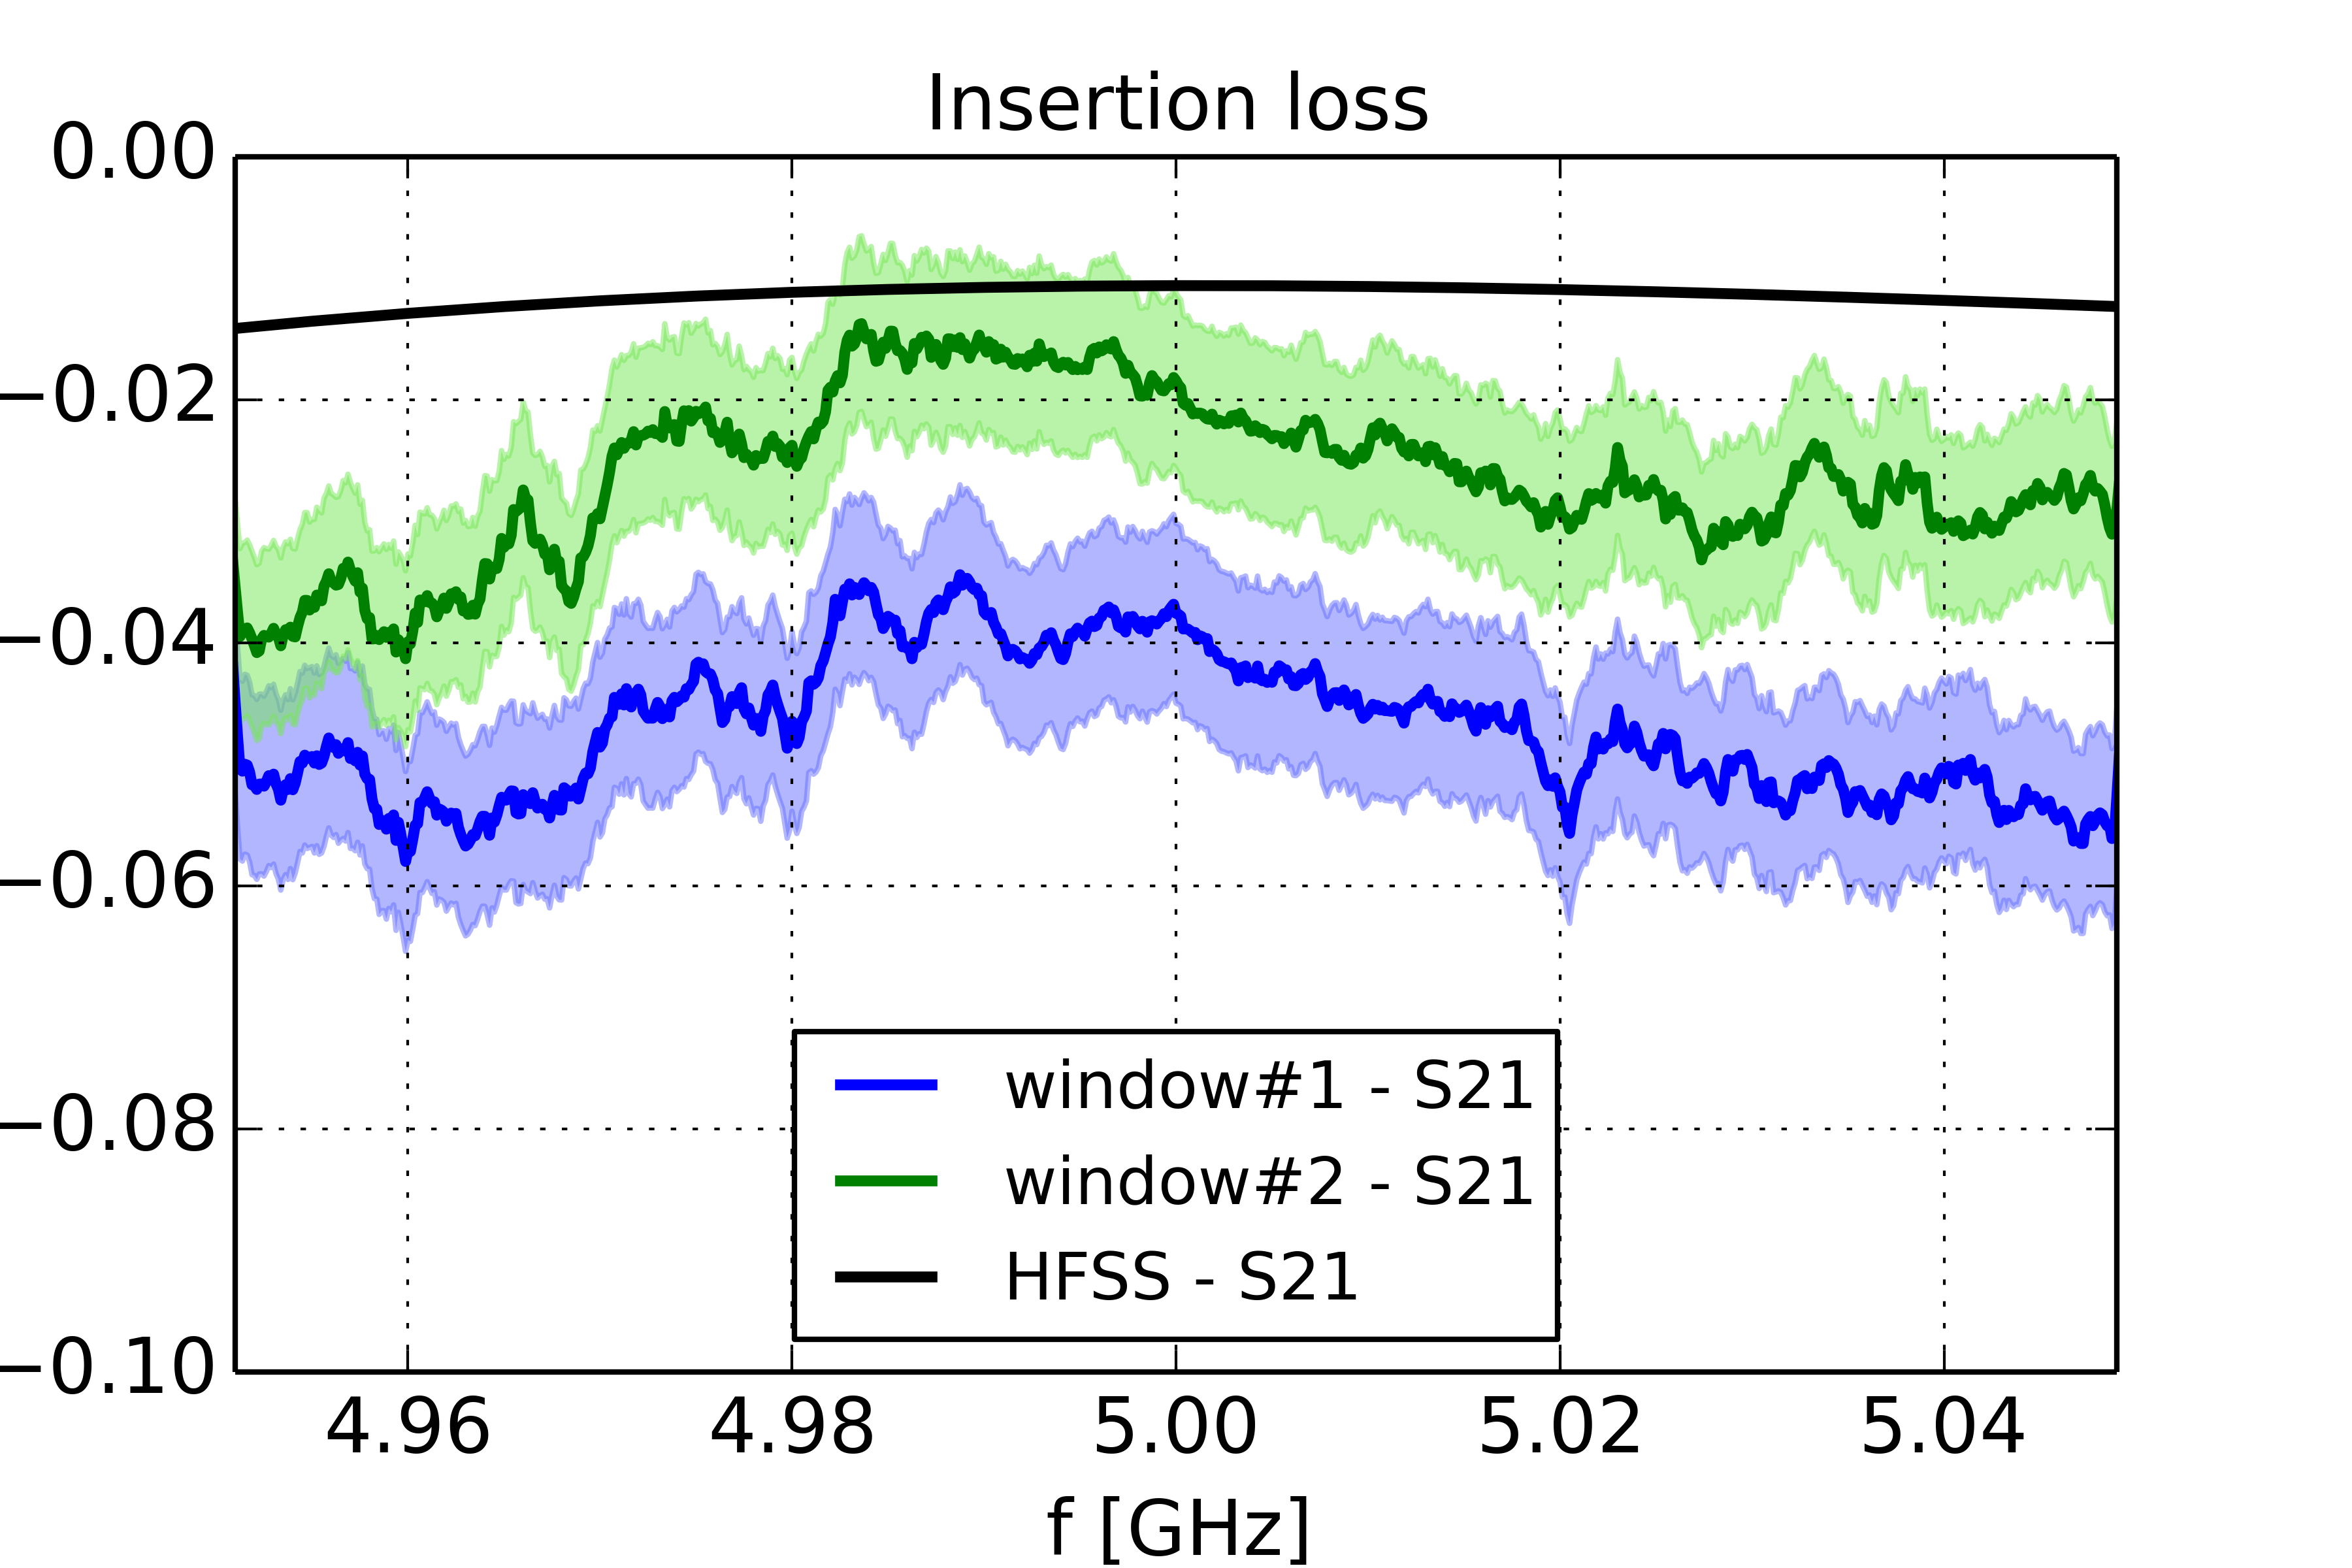
\includegraphics[width=1.0\linewidth]{figures/chap3/ITER_window/ITER_windows_IL}
	\caption{Insertion loss [dB] for both windows. RF modelling prediction(plain black) from HFSS. Bold line represent the averaged values and shaded areas the minimum and maximum of the measurement noise.}
	\label{fig:iterwindowsil}
\end{figure}


\subsection{High Power RF Tests}
High power measurements have been performed on the NFRI LH test bed in 2013 and 2014. The setup shown in Figure~\ref{fig:iterwindowsrftests} consists in a single window inserted in the transmission line. The transmission line is filled with SF6 gas. A vacuum test with both windows at the same time using an interspace pumping system was also expected in case of successful completion of the tests of both prototypes. The windows were cooled with 8 to 17~\si{L/min} water flow at 20-25$\si{\degreeCelsius}$. Calorimetric measurements of the window water cooling loop were recorded during shots and used to estimate the power losses in the window\sidecite{park2013}. The temperature of the ceramic core was monitored by an infra-red camera (Agema thermovision 900, spectral range 2-5.4 \si{µm}) during 500~kW RF power shots. The measured BeO temperature depends on the BeO emissivity which is unknown. An absolute temperature calibration has been performed between 24.3$\si{\degreeCelsius}$ to 81.$\si{\degreeCelsius}$ using electrical blanket heating and shows a linear trend. Higher temperatures are deduced assuming linear interpolation of the calibration curve. 

\begin{figure}
	\centering
	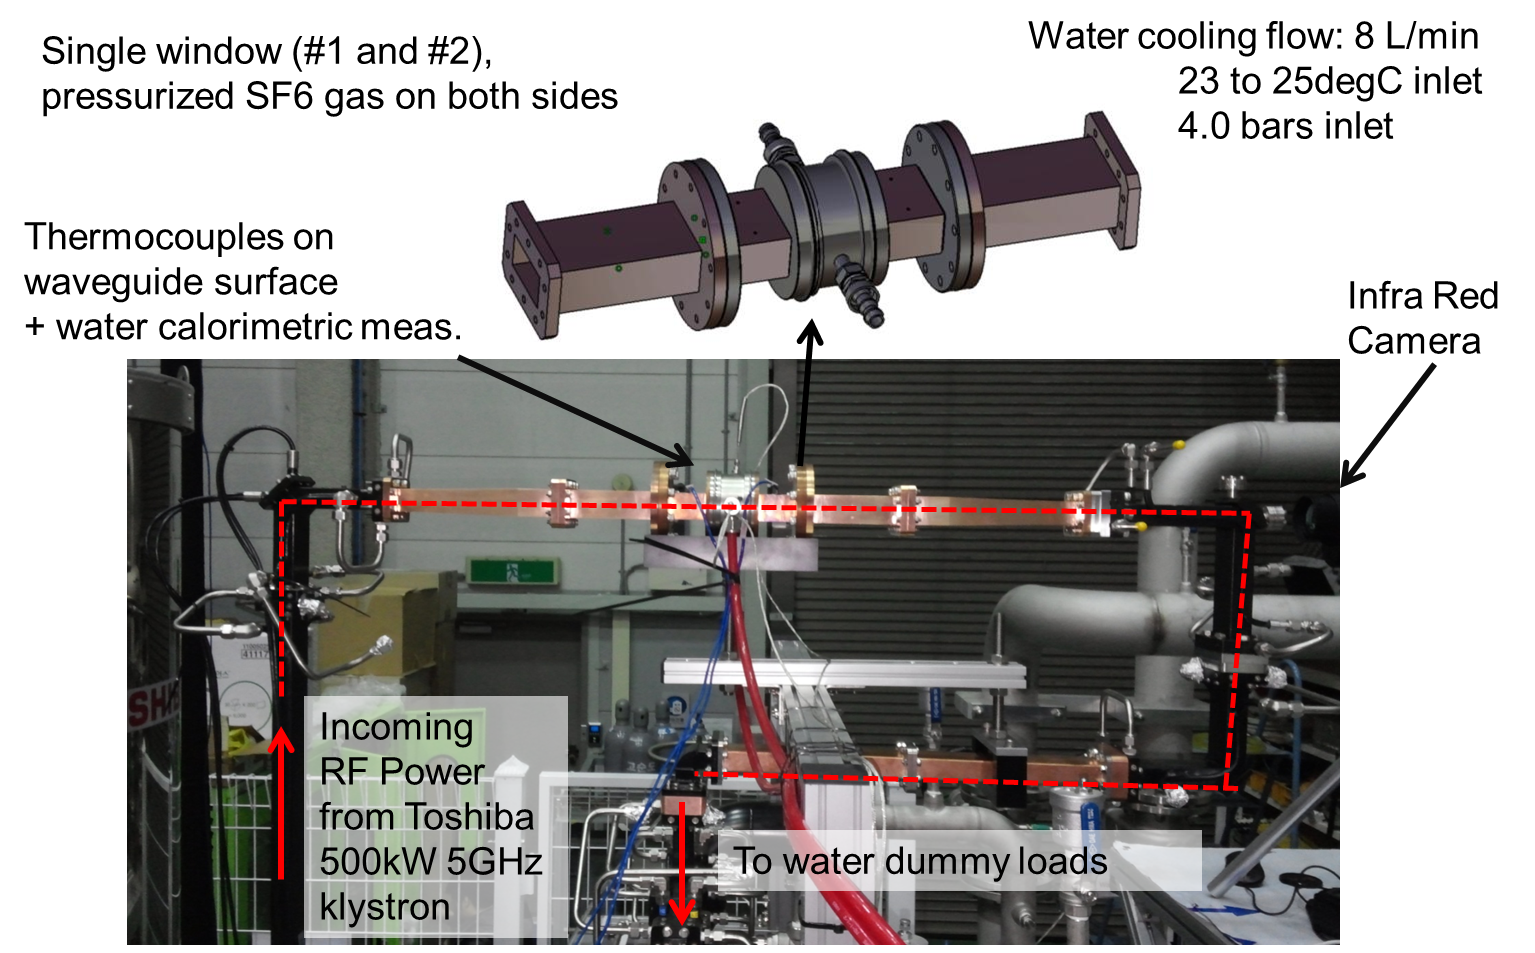
\includegraphics[width=1.0\linewidth]{figures/chap3/ITER_window/ITER_windows_RF_tests}
	\caption{High power test setup at 5GHz/500kW NFRI test bed in Korea.}
	\label{fig:iterwindowsrftests}
\end{figure}

The RF energy applied for both windows is illustrated in Figure~\ref{fig:iterwindowspulseenergy} as a function of the pulse number. The RF power has been applied during single pulses length of 100~ms starting from 25~kW, and then the power was increased progressively pulse by pulse by 25~kW steps up to 250~kW. RF pulse length has been increased progressively (in more than 30~pulses) up to 2.5~s at a power of 250~kW. The RF power has been increased up to 500~kW during 100~ms pulses, then the pulse length have been increased to few seconds at 500~kW, in more than 50 pulses. Repetitive pulses at 500 kW have been performed for different pulse lengths. A single breakdown event has been detected via the optical fiber protection system at 250~kW. The fraction of reflected power measured close to the klystron output ranged from -22.6~dB to -21.6~dB (VSWR 1.16:1 to 1.18:1) for the first window and from -21.2~dB to -20.8~dB (VSWR 1.19:1 to 1.2:1) for the second window. It has to be noted that the return losses are inclusive of the return losses produces by both the window and the whole assembly, including its various components such as bends and water loads, for which a -24.9~dB (VSWR 1.12:1) return loss has been measured without the window installed in the transmission line.

\begin{figure}
	\centering
	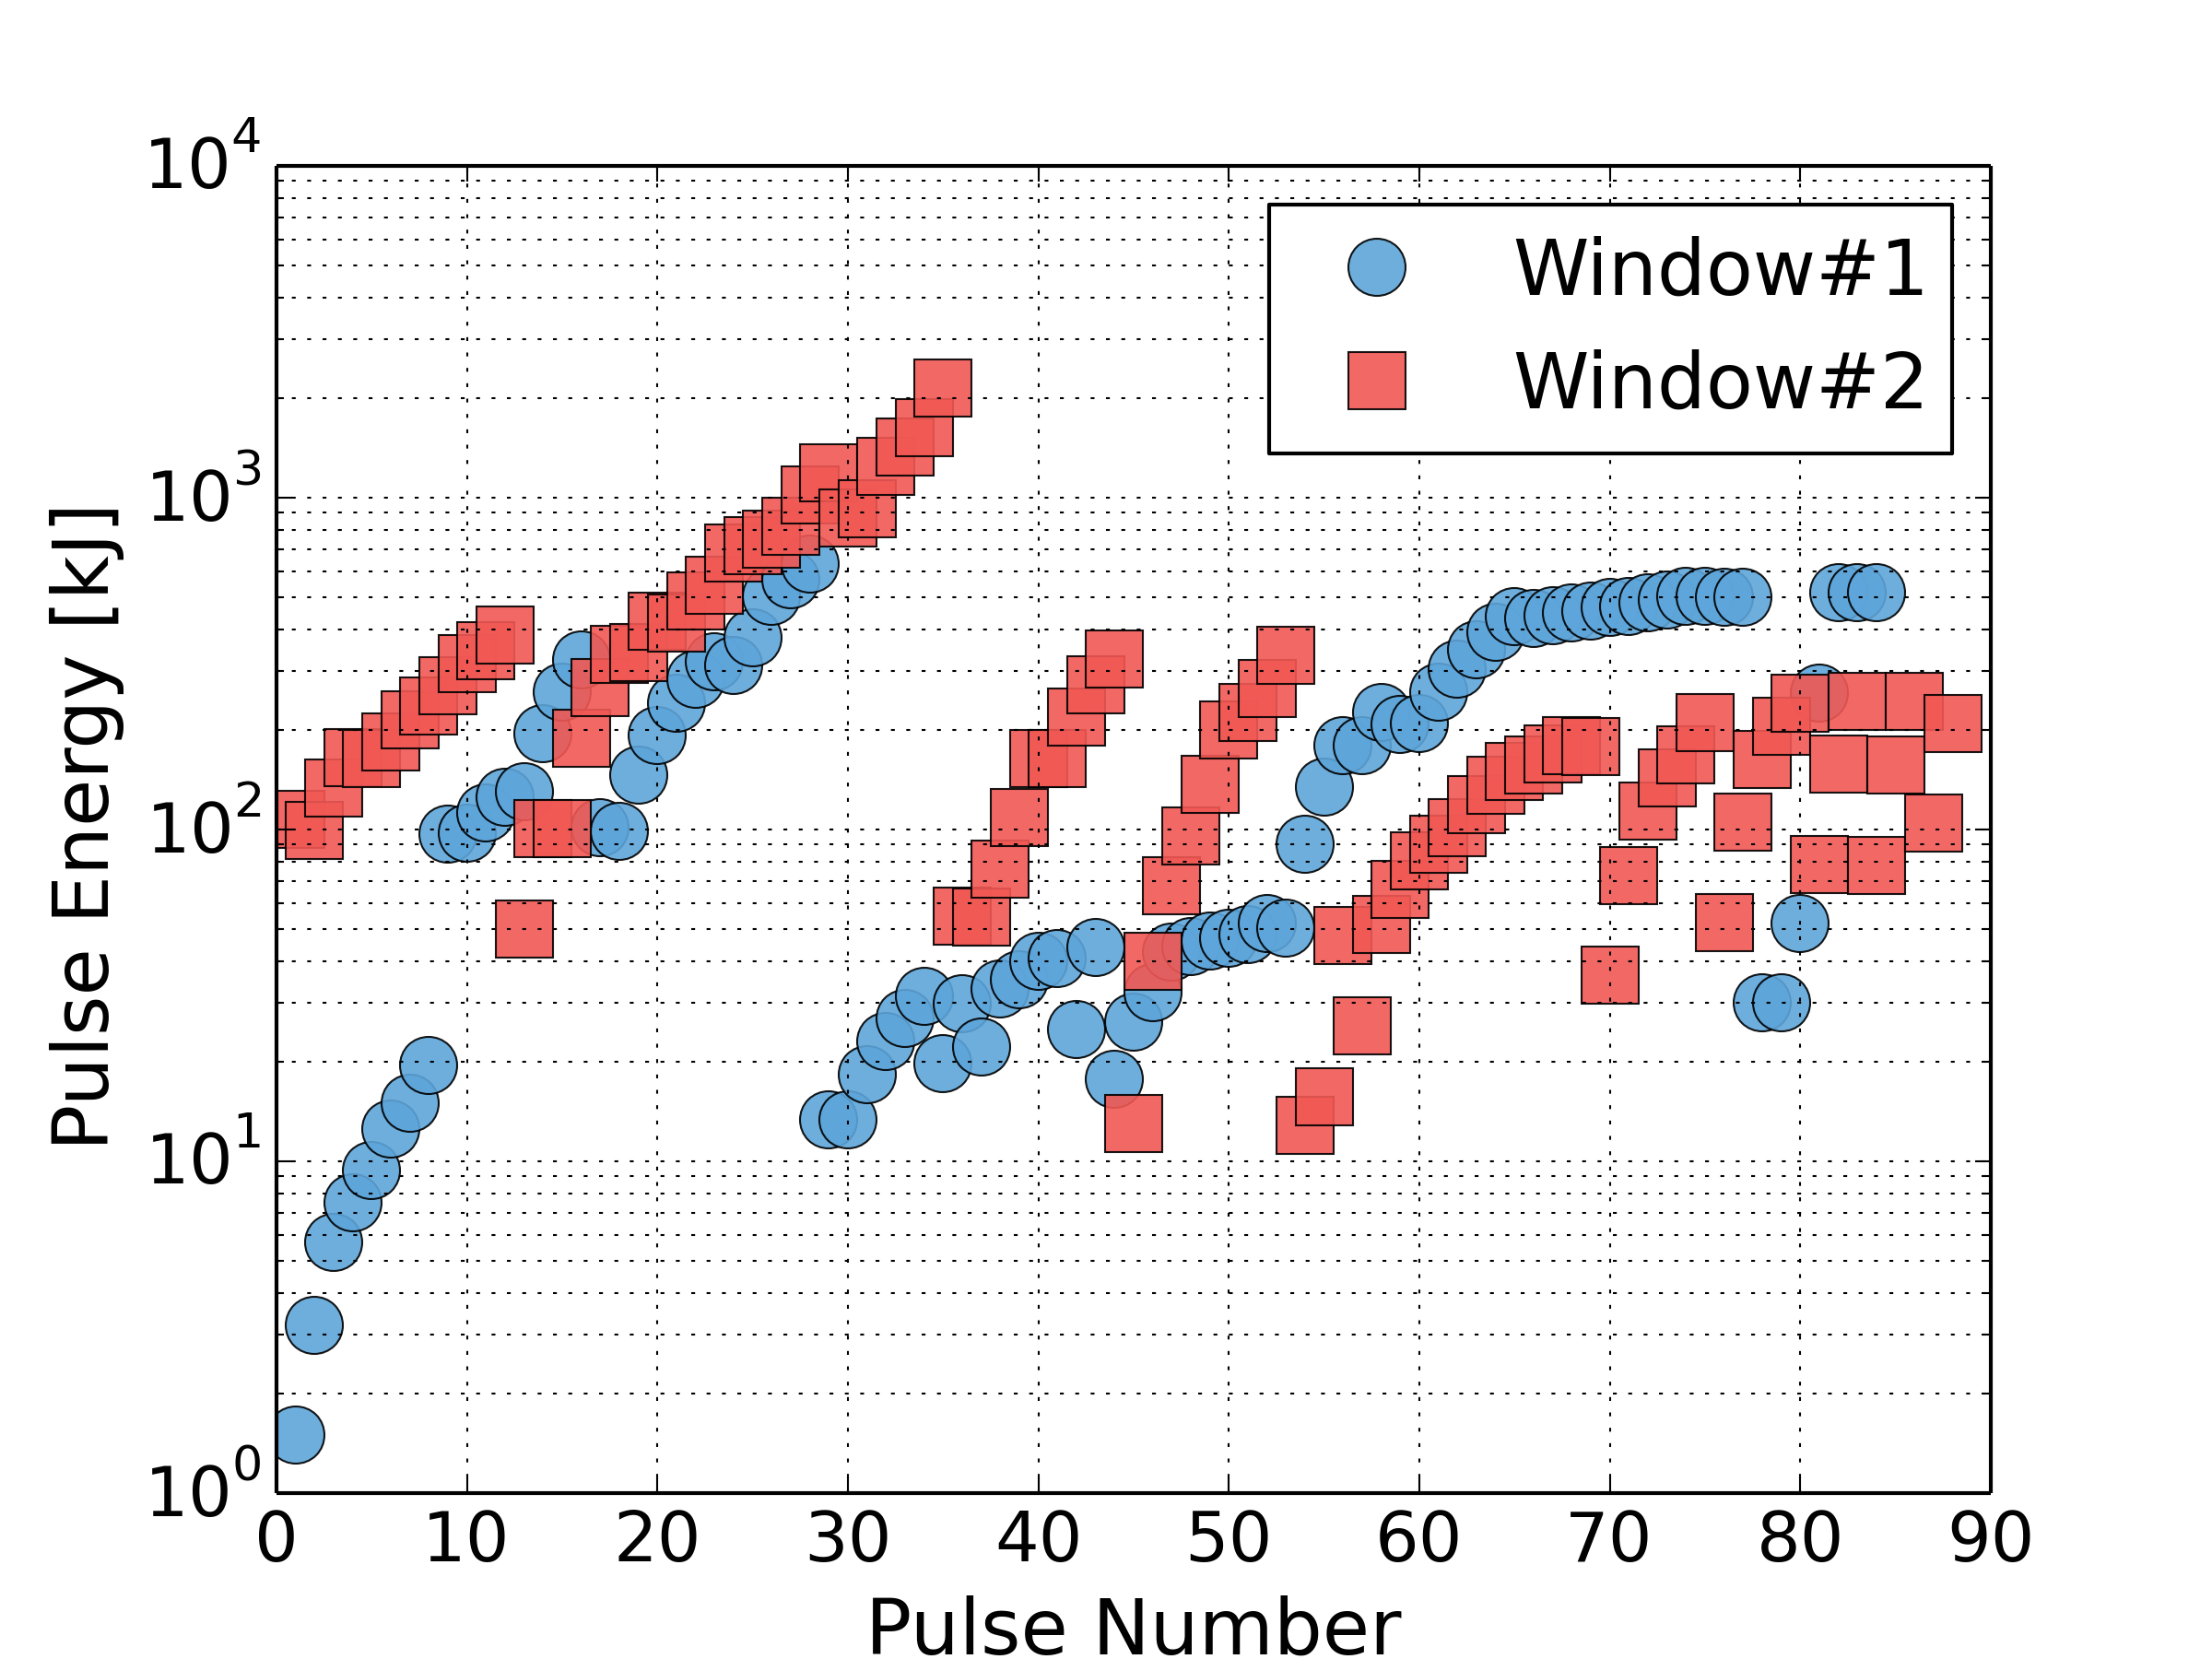
\includegraphics[width=1.0\linewidth]{figures/chap3/ITER_window/ITER_windows_pulse_energy}
	\caption{Pulse Energy in kJ as a function of the pulse number for both windows.}
	\label{fig:iterwindowspulseenergy}
\end{figure}

The water temperature increase $\Delta T$ during the RF power application from calorimetric measurement indicated a power loss in the device from 0.89\% to 1.1\% of the input power for the first window and of 0.7\% for the second window. This power loss includes the ceramic but also all the neighbouring copper-plated waveguide sections at both sides of the window, which were not water-cooled during these tests. This value is well above the 0.2\% expected from RF modelling or best measured values, but is consistent with the lowest range of values from low-power measurements reported in Section~\ref{sec:ITER_windows_manuf_low_power_tests}. These values are also in the same range of the ones measured on the Toshiba 5 GHz RF windows which equipped the klystron\sidecite{kim2019-2} . Total loss versus input power for both windows is reported in Figure 14 and shows linear trends. Two trend curves are related to the first window (1.1\% and 0.89\% of the incident power Pin) and the third one to the second window (0.73\% of Pin). The total losses are larger in the first window than in the second window, in consistence with low power measurements. The difference in the trends for the first window is not explained and is thought to come from measurement dispersion. These linear trends exclude eventual non-linear loss processes during these short-length pulses (up to 5 s). 

\begin{figure}
	\centering
	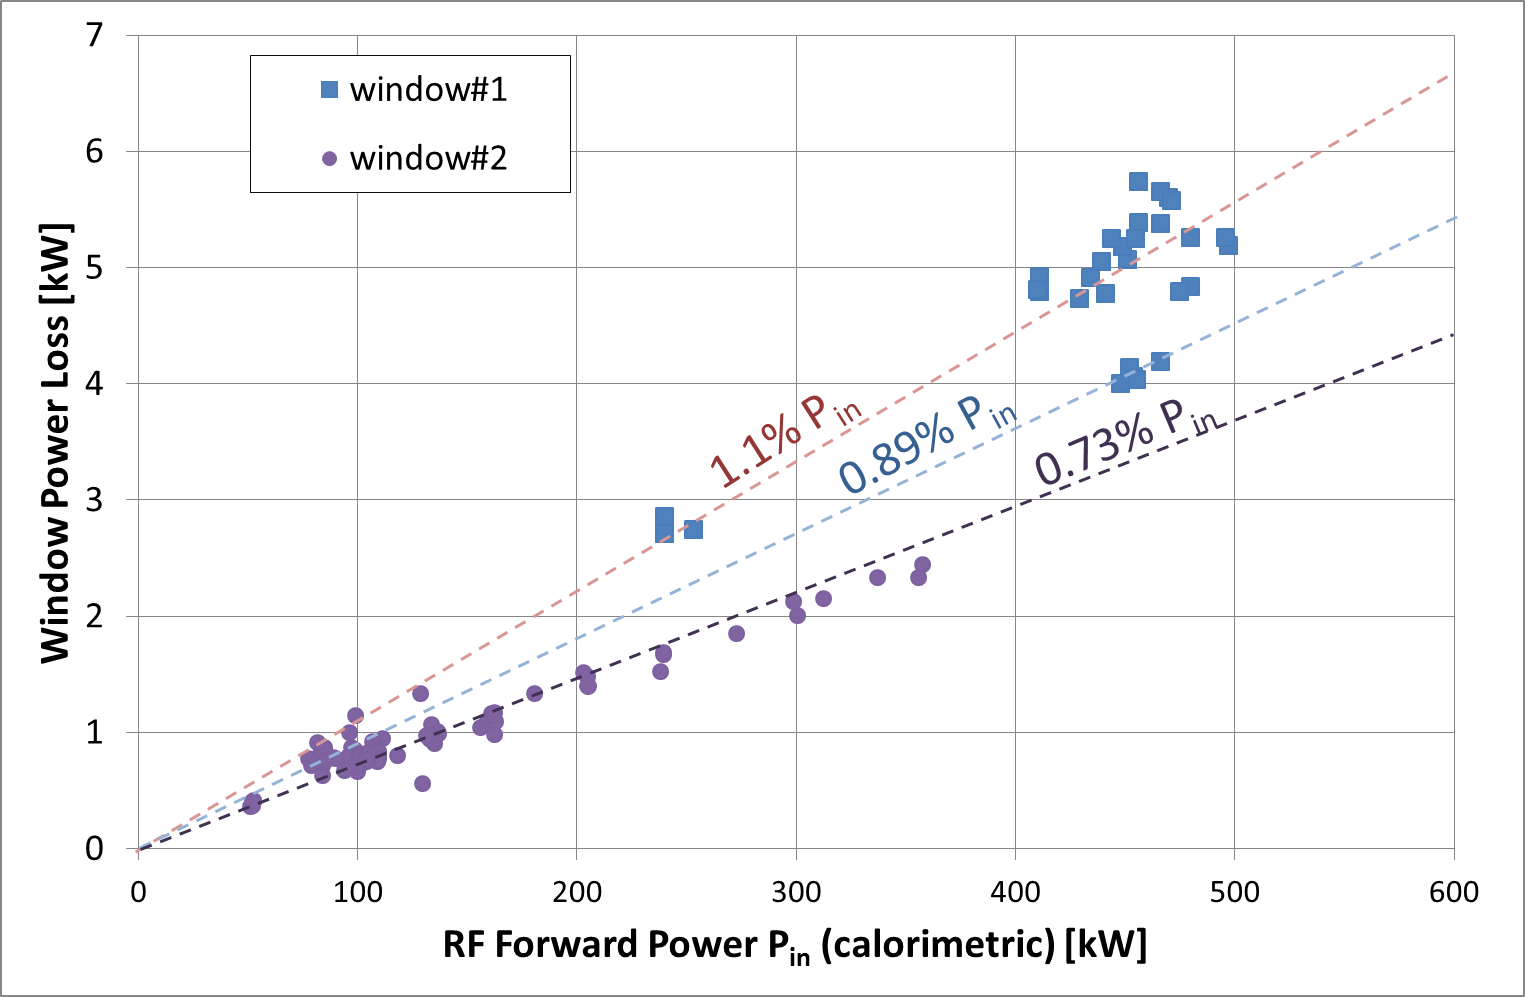
\includegraphics[width=1.0\linewidth]{figures/chap3/ITER_window/ITER_windows_power_loss}
	\caption{Measured calorimetric power losses for both prototype windows VS forward RF power Pin from dummy loads calorimetric measurement during the different experimental days}
	\label{fig:iterwindowspowerloss}
\end{figure}

Infra-red (IR) measurements of the ceramic temperature have been made during high power pulses.  The rods small diameter (1.6 mm) makes its temperature measurement difficult because of the camera resolution, but also mainly because of the IR reflections occurring on them. When the ceramic temperature is increasing, the rods become undistinguishable from the ceramic. Some thermocouples have been placed at the top of the window (cf Figure~\ref{fig:iterwindowsgeometry}), located specifically over the matching rods, but no change of temperature during the pulses was measured, in agreement with modelling. The ceramic central temperature (maximum temperature), measured by the IR camera after 3 seconds pulses at 500 kW (Figure 15), is recurrently higher than 250$\si{\degreeCelsius}$, and thus higher than the thermal modelling prediction illustrated in Figure 8 which was below 100$\si{\degreeCelsius}$ after a 5 s pulse. 

\begin{figure}
	\centering
	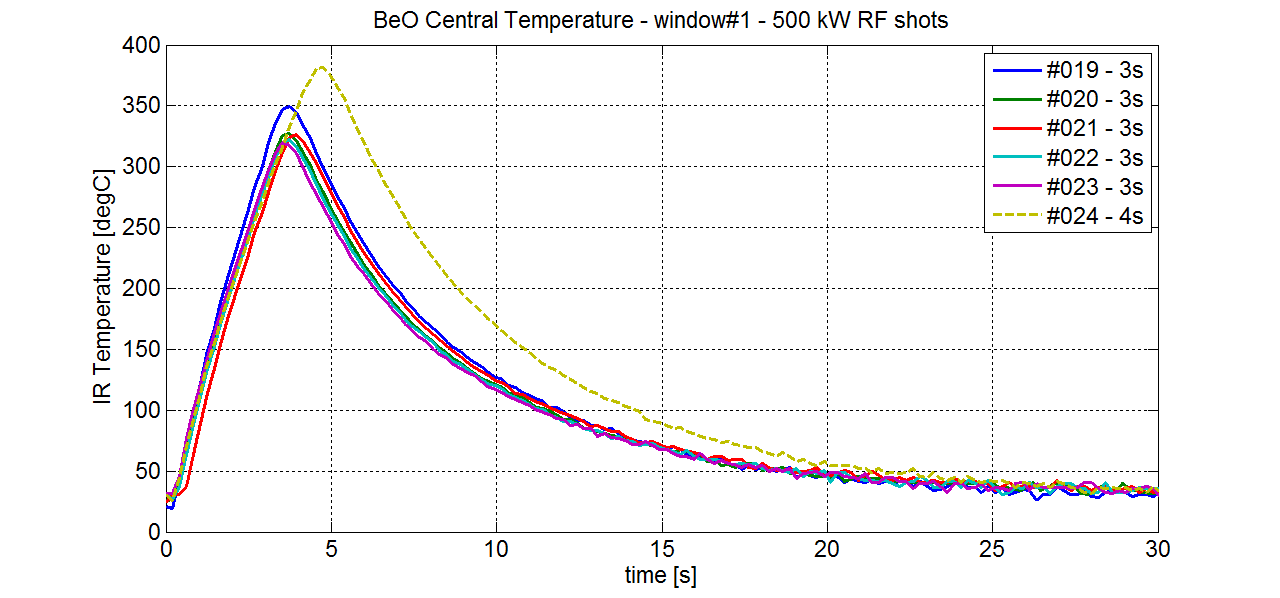
\includegraphics[width=1.0\linewidth]{figures/chap3/ITER_window/ITER_windows_BeO_temperature}
	\caption{BeO Central temperature evolution 3 s and 4 s shots, measured by the IR Camera for 500 kW±20kW input shots for window \#1.}
	\label{fig:iterwindowsbeotemperature}
\end{figure}

Moreover, the cooling time constant is around twice larger than expected from ideal thermal modelling, indicating that a thermal barrier reduces the heat conduction efficiency. The losses are not affected by a degradation of the cooling efficiency as the dissupated power does not depend on the thermal conductivity (if we assume that the dielectric loss tangent does not change with the temperature increase). 

The fact that the BeO central temperature increases to temperatures higher than 300$\si{\degreeCelsius}$ prevent these two windows prototype to be used in CW regime at full power without exceeding the mechanical stress limits of the ceramic. The first ceramic window prototype was found to be cracked after disassembly from the test-bed. Following this observation, the maximum power and the pulse length has been reduced for the following tests of the second window, in order not to exceed a maximum IR measured temperature of 100$\si{\degreeCelsius}$ to avoid high temperature gradient between the ceramic core and its periphery cooled by the 20-25$\si{\degreeCelsius}$ water loop. 



\subsection{Experimental Results Analysis}

Following the high power tests, two 16 mm diameter samples have been machined from the first (cracked) BeO ceramic window. A post-mortem RF analysis of these two samples has been performed with the same methodology used for the manufacturer sample (Cf. Section\ref{sec:ITER_windows_manuf_low_power_tests}). The relative permittivity measured on these two pieces was $6.74\pm0.12$ and $6.72\pm0.01$, to be compared with the 6.36 value originally measured on the manufacturer sample. The $\tan \delta$ was also up to twice higher than expected from the BeO sample measurement (from $5.4\times10^{-4}$ up to $8.8\times10^{-4} \pm 1.1\times 10^{-5}$). RF modelling shows that the change of relative permittivity has little effect on the dielectric losses, indicating that no other higher order modes are excited in the ceramic. The change of permittivity shifts the optimum frequency by -20~MHz, which corroborates low power measurements (Figure~\ref{fig:iterwindowsrl}). A loss tangent value of $9\times10^{-4}$ leads to double the total losses in the ceramic. Doubling the dielectric loss tangent into an ideal thermal model leads to a BeO central temperature of nearly 140$\si{\degreeCelsius}$ after a 5~s pulse. However, even taking into account these changes in the reference RF model, the predicted total RF losses reach 2~kW, still far from the 5~kW and 2.5~kW measured by calorimetry for window \#1 and \#2 respectively. 

We observe in Figure~\ref{fig:iterwindowspowerloss} that the total losses are almost linear with respect to the input power, thus excluding any significant changes on the dielectric loss tangent or copper conductivity with temperature for these short-length pulses.  The effect of the reflected power from the waveguide bends and the water loads has been assessed and is marginal in the total RF losses evaluation. Adding small gaps between the bonded parts of the window or at the flange interfaces may possibly causes additional RF losses. However, a reliable estimate of these losses is difficult. As the power lost in the ceramic is linearly linked to the dielectric loss tangent, the latter is thought to be the dominant player.

As seen in Figure~\ref{fig:iterwindowsrftests}, the window is connected to copper waveguide adapters on both sides. Each side is the addition of two waveguide sections of 140~mm and 248~mm length respectively. As these waveguides attached to the window were not actively cooled, a fraction of the RF power lost into them participates to the power balance measured by the calorimetric method. With a realistic copper conductivity of $\sigma=44~\si{MS/m}$, the conduction losses  from Eq.(\ref{eq:rectwg_power_loss_per_unit_length}) for a WR229 waveguide at 5~GHz for 500~kW are 2.9~kW/m. Taking into account only the two 140 mm length waveguides, the power balance leads to an additional RF power loss of 810~W. Taking into account all the waveguides length (140~mm + 248~mm) the power balance leads to an additional RF power loss of 2300~W. However, estimating the real fraction of power lost in these waveguides and dissipated into the window water cooling loop is delicate because of the large uncertainty of the thermal contacts between flanges. 

Taking into account the post-mortem BeO RF properties in the RF model leads to an insertion loss of -0.02 dB (0.5\%) and -0.03 dB (0.7\%) if one includes the connection waveguides on each sides of the window. Modelling and measurements are then consistent if one assumes that between 5 and 20\% of the power measured by calorimetry is dissipated in the connection waveguides. These modelling however do not take into account the fact that the matching rods are slightly deformed.

The longer characteristic time measured from IR during cooling can be originated from either a decreased BeO thermal conductivity, a reduced water heat transfer coefficient or a thermal barrier between the BeO and the copper skirt. If the first two have little effect on the thermal modelling results, unless using non-realistic values, the latter is thought to be the main cause of a reduced cooling efficiency. The brazing layer is made of gold/copper alloys (Au50/Cu50) in order to avoid silver alloys, which are undesirable in ITER because of transmutation risks during the nuclear phase. This brazing material has a low thermal conductivity (in the order of 33~\si{W/m/K}). Moreover, in order to increase the wettability of the BeO to the brazing alloy, a metallization of the BeO periphery is performed using a Molybdenum/Manganese layer, with the addition of nickel plating. Both have also a low thermal conductivity. Taking into account the Molybdenum/Manganese layer which has an electrical conductivity about 6~MS/m in the RF model as an impedance boundary condition leads to increase the RF losses around the ceramic of about 10~W for 500~kW input. Thermal modelling of such brazing layers, which thickness is typically between 20 to 40~µm, is delicate and is highly sensitive to parameter values. However, the general trend when applying a degraded thermal contact at the interface between the BeO and the copper is a fast increase of the temperature rise time due to a thermal barrier effect and similarly an increase of the characteristic cooling time, both observed experimentally. 


\subsection{Summary of this section}
Two 5 GHz 500 kW/5 s windows have been designed and tested at high power in collaboration with NFRI. The window design relies on a symmetrical pill-box concept with a cylindrical beryllium oxide (BeO) ceramic brazed on an actively water cooled copper skirt. The ceramic RF properties have been measured on a manufacturer test sample in order to get realistic values for guiding the design. Low power measurements show return losses below -32 dB (VSWR < 1.05:1) and insertion losses between -0.01 dB and -0.05 dB (i.e. 0.23\% to 1.14\% of input power), with the optimum frequency shifted toward frequencies lower than the nominal one. High power tests conducted at NFRI show a total power loss of 1.1\% of the input power for one window and of 0.7\% for the second one, in agreement with the lowest range of cold RF measurement but not with initial RF simulations. These values are also in the same range than the ones measured on the two Toshiba 5 GHz RF windows which equipped the klystron. The ceramic temperature during RF pulses has been found to reach unexpected high values, preventing these windows to be used under CW conditions because of the ceramic stress limits. 

Post-mortem RF measurement of two BeO samples of one of the windows shows that the dielectric relative permittivity of the ceramic was 6.7 while for the sample initially measured it was 6.36. More important, the measured dielectric loss tangent on the two post-mortem ceramic samples is up to twice as high as the manufacturer sample. The difference in the permittivity explains the shift of the optimum frequency.  RF modelling including the new dielectric properties of BeO, a more realistic RF conduction loss rate on copper and the additional connection waveguides, shows that the calculated RF losses match the observations. However, the only increase of the dielectric loss is not sufficient to explain the high temperatures measured with infrared camera. The higher temperature and delay time is explained by a thermal barrier due to ceramic metallization and the use of low thermal conduction brazing materials. 

 
This work shows that large margins must be taken from the reference design (or alternatively accept large production wastes), especially in cases where mechanical stresses are close to acceptable margins. It is believed that improvements in the manufacturing (in particular the brazing of the ceramic) and in the water cooling circuit are necessary to achieve the target performances.  